\documentclass[10pt,twoside,openright]{memoir}
% remove page numbers
\let\footruleskip\relax

\usepackage[paperwidth=4.25in,paperheight=6.875in,bindingoffset=.15in,top=0.25in,bottom=0.25in,left=0.25in,right=0.25in]{geometry}

% remove page numbers
\usepackage{fancyhdr}
\fancypagestyle{plain}{
\fancyhf{}
\renewcommand{\headrulewidth}{0pt}
\renewcommand{\footrulewidth}{0pt}}

\setsecheadstyle{\large\bfseries}
\chapterstyle{section}
\renewcommand*{\chapnumfont}{\Large\bfseries}
\renewcommand*{\chaptitlefont}{\Large\bfseries}
\setlength\beforechapskip{0pt}
\setlength\afterchapskip{16pt}

% underlining; use \ul{}
\usepackage{soul}
\setuldepth{m}

\usepackage{graphicx}

% font
\usepackage[bitstream-charter]{mathdesign}
\usepackage[T1]{fontenc}

% sideways pages
\usepackage{pdflscape}

\setlength{\vleftmargin}{0em}

\usepackage{longtable}

% number figures continuously increasing through doc, not per-chapter
\counterwithout{figure}{chapter}
\renewcommand{\figurename}{Fig.}

% when a figure has no caption, show "Fig 1" not "Fig 1:"
\usepackage{caption}

% for backticks in verbatim
\usepackage{upquote}

% hyphenation tolerance; higher means less chance of overfull boxes
\tolerance=10000

% for fractions like 3/8
\usepackage{units}
% use \nicefrac{3}{8}


\setsecnumdepth{none}
\maxsecnumdepth{none}

\begin{document}

\pagestyle{empty}


\chapter{Beating the Averages (Paul Graham)}

In the summer of 1995, my friend Robert Morris and I started a startup called Viaweb. Our plan was to write software that would let end users build online stores. What was novel about this software, at the time, was that it ran on our server, using ordinary Web pages as the interface.

A lot of people could have been having this idea at the same time, of course, but as far as I know, Viaweb was the first Web-based application. It seemed such a novel idea to us that we named the company after it: Viaweb, because our software worked via the Web, instead of running on your desktop computer.

Another unusual thing about this software was that it was written primarily in a programming language called Lisp. It was one of the first big end-user applications to be written in Lisp, which up till then had been used mostly in universities and research labs.~[1]

\section{The Secret Weapon}

Eric Raymond has written an essay called "How to Become a Hacker," and in it, among other things, he tells would-be hackers what languages they should learn. He suggests starting with Python and Java, because they are easy to learn. The serious hacker will also want to learn C, in order to hack Unix, and Perl for system administration and cgi scripts. Finally, the truly serious hacker should consider learning Lisp:

\begin{quote}
Lisp is worth learning for the profound enlightenment experience you will have when you finally get it; that experience will make you a better programmer for the rest of your days, even if you never actually use Lisp itself a lot.
\end{quote}

This is the same argument you tend to hear for learning Latin. It won't get you a job, except perhaps as a classics professor, but it will improve your mind, and make you a better writer in languages you do want to use, like English.

But wait a minute. This metaphor doesn't stretch that far. The reason Latin won't get you a job is that no one speaks it. If you write in Latin, no one can understand you. But Lisp is a computer language, and computers speak whatever language you, the programmer, tell them to.

So if Lisp makes you a better programmer, like he says, why wouldn't you want to use it? If a painter were offered a brush that would make him a better painter, it seems to me that he would want to use it in all his paintings, wouldn't he? I'm not trying to make fun of Eric Raymond here. On the whole, his advice is good. What he says about Lisp is pretty much the conventional wisdom. But there is a contradiction in the conventional wisdom: Lisp will make you a better programmer, and yet you won't use it.

Why not? Programming languages are just tools, after all. If Lisp really does yield better programs, you should use it. And if it doesn't, then who needs it?

This is not just a theoretical question. Software is a very competitive business, prone to natural monopolies. A company that gets software written faster and better will, all other things being equal, put its competitors out of business. And when you're starting a startup, you feel this very keenly. Startups tend to be an all or nothing proposition. You either get rich, or you get nothing. In a startup, if you bet on the wrong technology, your competitors will crush you.

Robert and I both knew Lisp well, and we couldn't see any reason not to trust our instincts and go with Lisp. We knew that everyone else was writing their software in C++ or Perl. But we also knew that that didn't mean anything. If you chose technology that way, you'd be running Windows. When you choose technology, you have to ignore what other people are doing, and consider only what will work the best.

This is especially true in a startup. In a big company, you can do what all the other big companies are doing. But a startup can't do what all the other startups do. I don't think a lot of people realize this, even in startups.

The average big company grows at about ten percent a year. So if you're running a big company and you do everything the way the average big company does it, you can expect to do as well as the average big company -- that is, to grow about ten percent a year.

The same thing will happen if you're running a startup, of course. If you do everything the way the average startup does it, you should expect average performance. The problem here is, average performance means that you'll go out of business. The survival rate for startups is way less than fifty percent. So if you're running a startup, you had better be doing something odd. If not, you're in trouble.

Back in 1995, we knew something that I don't think our competitors understood, and few understand even now: when you're writing software that only has to run on your own servers, you can use any language you want. When you're writing desktop software, there's a strong bias toward writing applications in the same language as the operating system. Ten years ago, writing applications meant writing applications in C. But with Web-based software, especially when you have the source code of both the language and the operating system, you can use whatever language you want.

This new freedom is a double-edged sword, however. Now that you can use any language, you have to think about which one to use. Companies that try to pretend nothing has changed risk finding that their competitors do not.

If you can use any language, which do you use? We chose Lisp. For one thing, it was obvious that rapid development would be important in this market. We were all starting from scratch, so a company that could get new features done before its competitors would have a big advantage. We knew Lisp was a really good language for writing software quickly, and server-based applications magnify the effect of rapid development, because you can release software the minute it's done.

If other companies didn't want to use Lisp, so much the better. It might give us a technological edge, and we needed all the help we could get. When we started Viaweb, we had no experience in business. We didn't know anything about marketing, or hiring people, or raising money, or getting customers. Neither of us had ever even had what you would call a real job. The only thing we were good at was writing software. We hoped that would save us. Any advantage we could get in the software department, we would take.

So you could say that using Lisp was an experiment. Our hypothesis was that if we wrote our software in Lisp, we'd be able to get features done faster than our competitors, and also to do things in our software that they couldn't do. And because Lisp was so high-level, we wouldn't need a big development team, so our costs would be lower. If this were so, we could offer a better product for less money, and still make a profit. We would end up getting all the users, and our competitors would get none, and eventually go out of business. That was what we hoped would happen, anyway.

What were the results of this experiment? Somewhat surprisingly, it worked. We eventually had many competitors, on the order of twenty to thirty of them, but none of their software could compete with ours. We had a wysiwyg online store builder that ran on the server and yet felt like a desktop application. Our competitors had cgi scripts. And we were always far ahead of them in features. Sometimes, in desperation, competitors would try to introduce features that we didn't have. But with Lisp our development cycle was so fast that we could sometimes duplicate a new feature within a day or two of a competitor announcing it in a press release. By the time journalists covering the press release got round to calling us, we would have the new feature too.

It must have seemed to our competitors that we had some kind of secret weapon -- that we were decoding their Enigma traffic or something. In fact we did have a secret weapon, but it was simpler than they realized. No one was leaking news of their features to us. We were just able to develop software faster than anyone thought possible.

When I was about nine I happened to get hold of a copy of The Day of the Jackal, by Frederick Forsyth. The main character is an assassin who is hired to kill the president of France. The assassin has to get past the police to get up to an apartment that overlooks the president's route. He walks right by them, dressed up as an old man on crutches, and they never suspect him.

Our secret weapon was similar. We wrote our software in a weird AI language, with a bizarre syntax full of parentheses. For years it had annoyed me to hear Lisp described that way. But now it worked to our advantage. In business, there is nothing more valuable than a technical advantage your competitors don't understand. In business, as in war, surprise is worth as much as force.

And so, I'm a little embarrassed to say, I never said anything publicly about Lisp while we were working on Viaweb. We never mentioned it to the press, and if you searched for Lisp on our Web site, all you'd find were the titles of two books in my bio. This was no accident. A startup should give its competitors as little information as possible. If they didn't know what language our software was written in, or didn't care, I wanted to keep it that way.~[2]

The people who understood our technology best were the customers. They didn't care what language Viaweb was written in either, but they noticed that it worked really well. It let them build great looking online stores literally in minutes. And so, by word of mouth mostly, we got more and more users. By the end of 1996 we had about 70 stores online. At the end of 1997 we had 500. Six months later, when Yahoo bought us, we had 1070 users. Today, as Yahoo Store, this software continues to dominate its market. It's one of the more profitable pieces of Yahoo, and the stores built with it are the foundation of Yahoo Shopping. I left Yahoo in 1999, so I don't know exactly how many users they have now, but the last I heard there were about 20,000.

\section{The Blub Paradox}

What's so great about Lisp? And if Lisp is so great, why doesn't everyone use it? These sound like rhetorical questions, but actually they have straightforward answers. Lisp is so great not because of some magic quality visible only to devotees, but because it is simply the most powerful language available. And the reason everyone doesn't use it is that programming languages are not merely technologies, but habits of mind as well, and nothing changes slower. Of course, both these answers need explaining.

I'll begin with a shockingly controversial statement: programming languages vary in power.

Few would dispute, at least, that high level languages are more powerful than machine language. Most programmers today would agree that you do not, ordinarily, want to program in machine language. Instead, you should program in a high-level language, and have a compiler translate it into machine language for you. This idea is even built into the hardware now: since the 1980s, instruction sets have been designed for compilers rather than human programmers.

Everyone knows it's a mistake to write your whole program by hand in machine language. What's less often understood is that there is a more general principle here: that if you have a choice of several languages, it is, all other things being equal, a mistake to program in anything but the most powerful one.~[3]

There are many exceptions to this rule. If you're writing a program that has to work very closely with a program written in a certain language, it might be a good idea to write the new program in the same language. If you're writing a program that only has to do something very simple, like number crunching or bit manipulation, you may as well use a less abstract language, especially since it may be slightly faster. And if you're writing a short, throwaway program, you may be better off just using whatever language has the best library functions for the task. But in general, for application software, you want to be using the most powerful (reasonably efficient) language you can get, and using anything else is a mistake, of exactly the same kind, though possibly in a lesser degree, as programming in machine language.

You can see that machine language is very low level. But, at least as a kind of social convention, high-level languages are often all treated as equivalent. They're not. Technically the term "high-level language" doesn't mean anything very definite. There's no dividing line with machine languages on one side and all the high-level languages on the other. Languages fall along a continuum~[4] of abstractness, from the most powerful all the way down to machine languages, which themselves vary in power.

Consider Cobol. Cobol is a high-level language, in the sense that it gets compiled into machine language. Would anyone seriously argue that Cobol is equivalent in power to, say, Python? It's probably closer to machine language than Python.

Or how about Perl 4? Between Perl 4 and Perl 5, lexical closures got added to the language. Most Perl hackers would agree that Perl 5 is more powerful than Perl 4. But once you've admitted that, you've admitted that one high level language can be more powerful than another. And it follows inexorably that, except in special cases, you ought to use the most powerful you can get.

This idea is rarely followed to its conclusion, though. After a certain age, programmers rarely switch languages voluntarily. Whatever language people happen to be used to, they tend to consider just good enough.

Programmers get very attached to their favorite languages, and I don't want to hurt anyone's feelings, so to explain this point I'm going to use a hypothetical language called Blub. Blub falls right in the middle of the abstractness continuum. It is not the most powerful language, but it is more powerful than Cobol or machine language.

And in fact, our hypothetical Blub programmer wouldn't use either of them. Of course he wouldn't program in machine language. That's what compilers are for. And as for Cobol, he doesn't know how anyone can get anything done with it. It doesn't even have x (Blub feature of your choice).

As long as our hypothetical Blub programmer is looking down the power continuum, he knows he's looking down. Languages less powerful than Blub are obviously less powerful, because they're missing some feature he's used to. But when our hypothetical Blub programmer looks in the other direction, up the power continuum, he doesn't realize he's looking up. What he sees are merely weird languages. He probably considers them about equivalent in power to Blub, but with all this other hairy stuff thrown in as well. Blub is good enough for him, because he thinks in Blub.

When we switch to the point of view of a programmer using any of the languages higher up the power continuum, however, we find that he in turn looks down upon Blub. How can you get anything done in Blub? It doesn't even have y.

By induction, the only programmers in a position to see all the differences in power between the various languages are those who understand the most powerful one. (This is probably what Eric Raymond meant about Lisp making you a better programmer.) You can't trust the opinions of the others, because of the Blub paradox: they're satisfied with whatever language they happen to use, because it dictates the way they think about programs.

I know this from my own experience, as a high school kid writing programs in Basic. That language didn't even support recursion. It's hard to imagine writing programs without using recursion, but I didn't miss it at the time. I thought in Basic. And I was a whiz at it. Master of all I surveyed.

The five languages that Eric Raymond recommends to hackers fall at various points on the power continuum. Where they fall relative to one another is a sensitive topic. What I will say is that I think Lisp is at the top. And to support this claim I'll tell you about one of the things I find missing when I look at the other four languages. How can you get anything done in them, I think, without macros?~[5]

Many languages have something called a macro. But Lisp macros are unique. And believe it or not, what they do is related to the parentheses. The designers of Lisp didn't put all those parentheses in the language just to be different. To the Blub programmer, Lisp code looks weird. But those parentheses are there for a reason. They are the outward evidence of a fundamental difference between Lisp and other languages.

Lisp code is made out of Lisp data objects. And not in the trivial sense that the source files contain characters, and strings are one of the data types supported by the language. Lisp code, after it's read by the parser, is made of data structures that you can traverse.

If you understand how compilers work, what's really going on is not so much that Lisp has a strange syntax as that Lisp has no syntax. You write programs in the parse trees that get generated within the compiler when other languages are parsed. But these parse trees are fully accessible to your programs. You can write programs that manipulate them. In Lisp, these programs are called macros. They are programs that write programs.

Programs that write programs? When would you ever want to do that? Not very often, if you think in Cobol. All the time, if you think in Lisp. It would be convenient here if I could give an example of a powerful macro, and say there! how about that? But if I did, it would just look like gibberish to someone who didn't know Lisp; there isn't room here to explain everything you'd need to know to understand what it meant. In \emph{ANSI Common Lisp} I tried to move things along as fast as I could, and even so I didn't get to macros until page 160.

But I think I can give a kind of argument that might be convincing. The source code of the Viaweb editor was probably about 20-25\% macros. Macros are harder to write than ordinary Lisp functions, and it's considered to be bad style to use them when they're not necessary. So every macro in that code is there because it has to be. What that means is that at least 20-25\% of the code in this program is doing things that you can't easily do in any other language. However skeptical the Blub programmer might be about my claims for the mysterious powers of Lisp, this ought to make him curious. We weren't writing this code for our own amusement. We were a tiny startup, programming as hard as we could in order to put technical barriers between us and our competitors.

A suspicious person might begin to wonder if there was some correlation here. A big chunk of our code was doing things that are very hard to do in other languages. The resulting software did things our competitors' software couldn't do. Maybe there was some kind of connection. I encourage you to follow that thread. There may be more to that old man hobbling along on his crutches than meets the eye.

\section{Aikido for Startups}

But I don't expect to convince anyone (over 25) to go out and learn Lisp. The purpose of this article is not to change anyone's mind, but to reassure people already interested in using Lisp -- people who know that Lisp is a powerful language, but worry because it isn't widely used. In a competitive situation, that's an advantage. Lisp's power is multiplied by the fact that your competitors don't get it.

If you think of using Lisp in a startup, you shouldn't worry that it isn't widely understood. You should hope that it stays that way. And it's likely to. It's the nature of programming languages to make most people satisfied with whatever they currently use. Computer hardware changes so much faster than personal habits that programming practice is usually ten to twenty years behind the processor. At places like MIT they were writing programs in high-level languages in the early 1960s, but many companies continued to write code in machine language well into the 1980s. I bet a lot of people continued to write machine language until the processor, like a bartender eager to close up and go home, finally kicked them out by switching to a RISC instruction set.

Ordinarily technology changes fast. But programming languages are different: programming languages are not just technology, but what programmers think in. They're half technology and half religion.~[6] And so the median language, meaning whatever language the median programmer uses, moves as slow as an iceberg. Garbage collection, introduced by Lisp in about 1960, is now widely considered to be a good thing. Runtime typing, ditto, is growing in popularity. Lexical closures, introduced by Lisp in the early 1970s, are now, just barely, on the radar screen. Macros, introduced by Lisp in the mid 1960s, are still terra incognita.

Obviously, the median language has enormous momentum. I'm not proposing that you can fight this powerful force. What I'm proposing is exactly the opposite: that, like a practitioner of Aikido, you can use it against your opponents.

If you work for a big company, this may not be easy. You will have a hard time convincing the pointy-haired boss to let you build things in Lisp, when he has just read in the paper that some other language is poised, like Ada was twenty years ago, to take over the world. But if you work for a startup that doesn't have pointy-haired bosses yet, you can, like we did, turn the Blub paradox to your advantage: you can use technology that your competitors, glued immovably to the median language, will never be able to match.

If you ever do find yourself working for a startup, here's a handy tip for evaluating competitors. Read their job listings. Everything else on their site may be stock photos or the prose equivalent, but the job listings have to be specific about what they want, or they'll get the wrong candidates.

During the years we worked on Viaweb I read a lot of job descriptions. A new competitor seemed to emerge out of the woodwork every month or so. The first thing I would do, after checking to see if they had a live online demo, was look at their job listings. After a couple years of this I could tell which companies to worry about and which not to. The more of an IT flavor the job descriptions had, the less dangerous the company was. The safest kind were the ones that wanted Oracle experience. You never had to worry about those. You were also safe if they said they wanted C++ or Java developers. If they wanted Perl or Python programmers, that would be a bit frightening -- that's starting to sound like a company where the technical side, at least, is run by real hackers. If I had ever seen a job posting looking for Lisp hackers, I would have been really worried.

\section{Notes}

[1] Viaweb at first had two parts: the editor, written in Lisp, which people used to build their sites, and the ordering system, written in C, which handled orders. The first version was mostly Lisp, because the ordering system was small. Later we added two more modules, an image generator written in C, and a back-office manager written mostly in Perl.

In January 2003, Yahoo released a new version of the editor written in C++ and Perl. It's hard to say whether the program is no longer written in Lisp, though, because to translate this program into C++ they literally had to write a Lisp interpreter: the source files of all the page-generating templates are still, as far as I know, Lisp code. (See Greenspun's Tenth Rule.)

[2] Robert Morris says that I didn't need to be secretive, because even if our competitors had known we were using Lisp, they wouldn't have understood why: "If they were that smart they'd already be programming in Lisp."

[3] All languages are equally powerful in the sense of being Turing equivalent, but that's not the sense of the word programmers care about. (No one wants to program a Turing machine.) The kind of power programmers care about may not be formally definable, but one way to explain it would be to say that it refers to features you could only get in the less powerful language by writing an interpreter for the more powerful language in it. If language A has an operator for removing spaces from strings and language B doesn't, that probably doesn't make A more powerful, because you can probably write a subroutine to do it in B. But if A supports, say, recursion, and B doesn't, that's not likely to be something you can fix by writing library functions.

[4] Note to nerds: or possibly a lattice, narrowing toward the top; it's not the shape that matters here but the idea that there is at least a partial order.

[5] It is a bit misleading to treat macros as a separate feature. In practice their usefulness is greatly enhanced by other Lisp features like lexical closures and rest parameters.

[6] As a result, comparisons of programming languages either take the form of religious wars or undergraduate textbooks so determinedly neutral that they're really works of anthropology. People who value their peace, or want tenure, avoid the topic. But the question is only half a religious one; there is something there worth studying, especially if you want to design new languages.


\chapter{Lisp Metacircular Evaluator}

\begin{center}
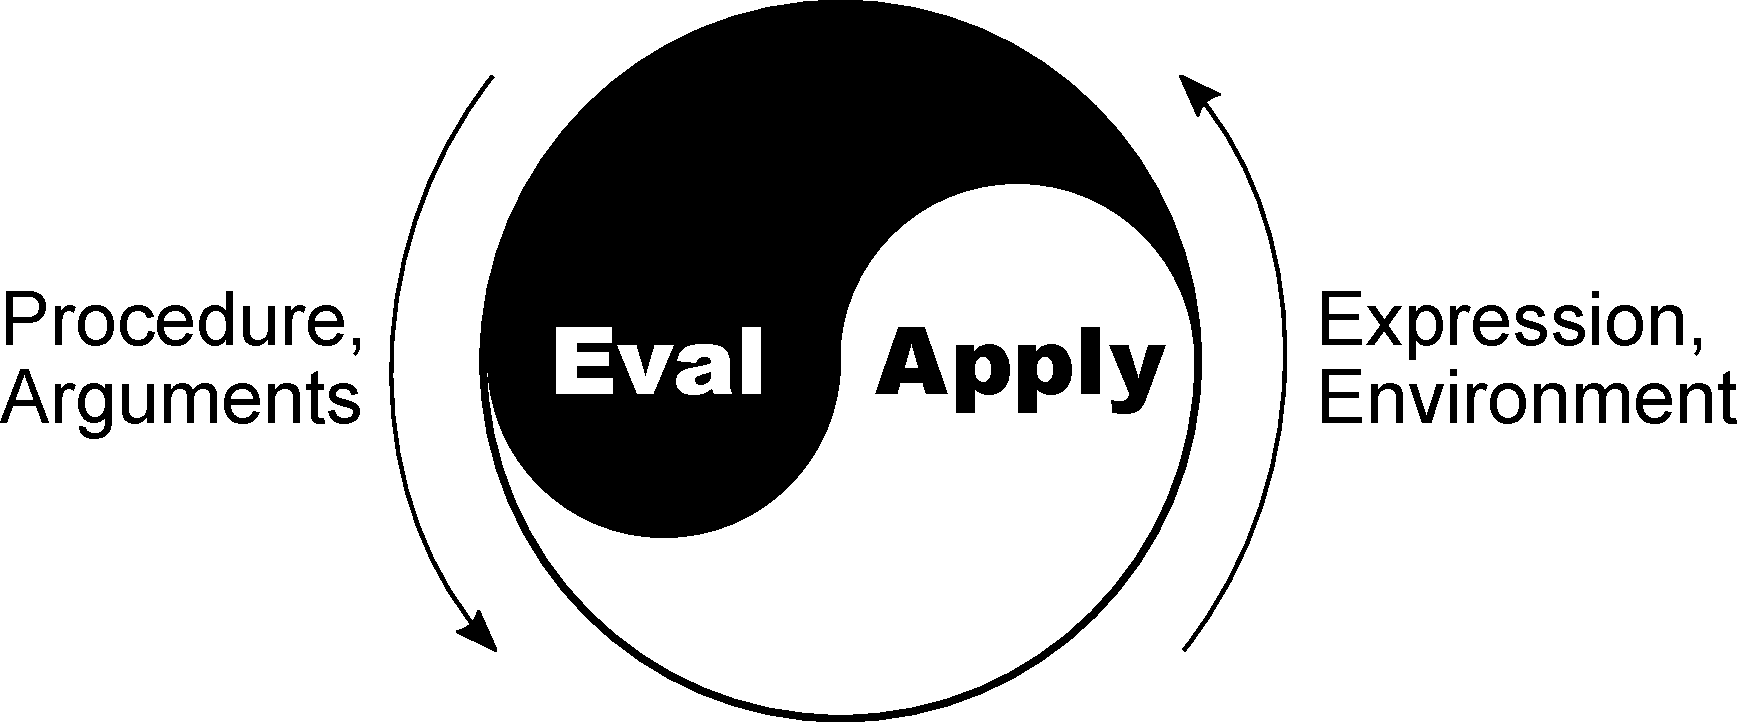
\includegraphics[scale=0.25]{figures/eval-apply.pdf}
\end{center}

{\footnotesize
\begin{verbatim}
(define (eval exp env)
  (cond ((self-evaluating? exp) exp)
        ((variable? exp) (lookup-variable-value exp env))
        ((quoted? exp) (text-of-quotation exp))
        ((assignment? exp) (eval-assignment exp env))
        ((definition? exp) (eval-definition exp env))
        ((if? exp) (eval-if exp env))
        ((lambda? exp)
         (make-procedure (lambda-parameters exp)
                         (lambda-body exp)
                         env))
        ((begin? exp) 
         (eval-sequence (begin-actions exp) env))
        ((cond? exp) (eval (cond->if exp) env))
        ((application? exp)
         (apply (eval (operator exp) env)
                (list-of-values (operands exp) env)))
        (else
         (error "Unknown expression type - EVAL" exp))))  

(define (apply procedure arguments)
  (cond ((primitive-procedure? procedure)
         (apply-primitive-procedure procedure arguments))
        ((compound-procedure? procedure)
         (eval-sequence
           (procedure-body procedure)
           (extend-environment
             (procedure-parameters procedure)
             arguments
             (procedure-environment procedure))))
        (else
         (error
          "Unknown procedure type - APPLY" procedure))))  
\end{verbatim}
}


\chapter{Powers of 2}

{\footnotesize
\begin{tabular}{rrrr}
0 & 1 & 1 & 1 \\
1 & 2 & 2 & 2 \\
2 & 4 & 4 & 4 \\
3 & 8 & 8 & 10 \\
4 & 16 & 10 & 20 \\
5 & 32 & 20 & 40 \\
6 & 64 & 40 & 100 \\
7 & 128 & 80 & 200 \\
8 & 256 & 100 & 400 \\
9 & 512 & 200 & 1000 \\
10 & 1,024 & 400 & 2000 \\
11 & 2,048 & 800 & 4000 \\
12 & 4,096 & 1000 & 10000 \\
13 & 8,192 & 2000 & 20000 \\
14 & 16,384 & 4000 & 40000 \\
15 & 32,768 & 8000 & 100000 \\
16 & 65,536 & 10000 & 200000 \\
17 & 131,072 & 20000 & 400000 \\
18 & 262,144 & 40000 & 1000000 \\
19 & 524,288 & 80000 & 2000000 \\
20 & 1,048,576 & 100000 & 4000000 \\
21 & 2,097,152 & 200000 & 10000000 \\
22 & 4,194,304 & 400000 & 20000000 \\
23 & 8,388,608 & 800000 & 40000000 \\
24 & 16,777,216 & 1000000 & 100000000 \\
25 & 33,554,432 & 2000000 & 200000000 \\
26 & 67,108,864 & 4000000 & 400000000 \\
27 & 134,217,728 & 8000000 & 1000000000 \\
28 & 268,435,456 & 10000000 & 2000000000 \\
29 & 536,870,912 & 20000000 & 4000000000 \\
30 & 1,073,741,824 & 40000000 & 10000000000 \\
31 & 2,147,483,648 & 80000000 & 20000000000 \\
32 & 4,294,967,296 & 100000000 & 40000000000 \\
\end{tabular}
}

\vskip 0.3in

{\footnotesize
\begin{verbatim}
base =: dyad define
syms =. ((48 + i. 10),(65 + i.0>.x-10)) { a.
idxs =. ((1+>.x^.y)#x)#:y
idxs { syms
)
b=:10 16 8
n=:33
(|:((#b),n)$n#b)base"0((n,#b)$(#b)#(2^i.n))
\end{verbatim}
}


\chapter{tmux}

{\footnotesize

Note, \texttt{C-} means Ctrl, e.g., \texttt{C-b} is Ctrl-b.

\vskip 0.2in

\noindent \begin{tabular}{ll}
\texttt{tmux} & start new session \\
\texttt{tmux new -s [name]} & start new session with name \\
\texttt{tmux attach} & attach to most recent session \\
\texttt{tmux attach -t [name]} & attach to named session \\
\texttt{tmux ls} & list sessions \\
\texttt{tmux kill-session -t [name]} & kill a named session \\
& \\
\texttt{C-b c} & create window \\
\texttt{C-b w} & list windows \\
\texttt{C-b n} & next window \\
\texttt{C-b p} & previous window \\
\texttt{C-b ,} & set name for window \\
\texttt{C-b \&} & kill window \\
\texttt{C-b d} & detach \\
& \\
\texttt{C-b \%} & split pane (vsplit) \\
\texttt{C-b "} & split pane (hsplit) \\
\texttt{C-b o} & switch panes \\
\texttt{C-b x} & kill pane \\
\texttt{C-b +} & change pane into window \\
\texttt{C-b -} & restore pane from window \\
\texttt{C-b [} & copy and scrollback mode \\
\texttt{C-b ?} & show key commands \\
\end{tabular}
}


\chapter{Vim}

{\footnotesize
\begin{tabular}{ll}
\texttt{0 \^{} \$} & move to front of line, first char, end \\
\texttt{h j k l} & move left, down, up, right \\
\texttt{w W} & move forward to start of words w/wo punc \\
\texttt{e E} & move forward to end of words w/wo punc \\
\texttt{b B} & move backward by word w/wo punc \\
\texttt{\} \{} & move forward/backward by paragraph \\
\texttt{\%} & move to matching (), \{\}, [] \\
\texttt{gg G} & move to top/bottom of file \\
\texttt{:[num][enter]} & move to line number \\
\texttt{/[regex]} & search forward for regex and move to first match \\
\texttt{?[regex]} & search backward for regex and move to last match \\
\texttt{n N} & repeat prior search in same / opposite direction \\
& \\
\texttt{i I} & insert at cursor, beginning of line \\
\texttt{a A} & append after cursor, end of line \\
\texttt{o O} & open blank line below, above current line \\
& \\
\texttt{c[move] cc} & change until move point, entire line \\
\texttt{d[move] dd} & delete until move point, entire line \\
\texttt{y[move] yy} & yank (copy) until move point, entire line \\
\texttt{p P} & put (paste) yanked content after / before cursor \\
\texttt{x X} & delete current / previous character \\
\texttt{r R} & replace a single character, multiple characters\\
\texttt{:s/[old]/[new]/g} & replace text on this line; \texttt{g} for all occurrences \\
\texttt{:\%s/[old]/[new]/g} & replace text in file; \texttt{g} for all occurrences \\
& \\
\texttt{=[move] ==} & auto-indent lines \\
\texttt{<[move] <{}<} & unindent one step \\
\texttt{>[move] >{}>} & indent one step \\
\texttt{:![cmd]} & pipe file through shell command, e.g., \texttt{:!sort} \\
& \\
\texttt{:w :wq ZZ} & write, write and quit, write and quit \\
\texttt{:q :q!} & quit, quit even if unsaved changes \\
\texttt{:e :ls :buf [num]} & edit another file, list buffers, switch to buffer \\
\texttt{:vsplit :hsplit} & split window \\
\texttt{Ctrl-w [hjkl]} & switch window \\
\texttt{u Ctrl+r .} & undo, redo, repeat last action \\
\end{tabular}

\vskip 0.1in
\noindent
Nearly all commands support a prefix number, e.g., \texttt{5dd} delete 5 lines.
}


\chapter{Emacs}

{\footnotesize
Note, \texttt{C-} means Ctrl- and \texttt{M-} means Meta- (Alt- or Esc-).

\vskip 0.2in

\noindent \begin{tabular}{ll}
\texttt{C-f C-b} & move forward, backward one character \\
\texttt{C-n C-p} & move down, up one line \\
\texttt{M-f M-b} & move forward, backward one word \\
\texttt{C-a C-e} & move to beginning, end of line \\
\texttt{M-a M-e} & move to beginning, end of sentence \\
\texttt{M-\{ M-\}} & move to beginning, end of paragraph \\
\texttt{M-< M->} & move to beginning, end of buffer \\
\texttt{C-v M-v} & page down, page up \\
\texttt{M-g g} & go to line \\
& \\
\texttt{C-d Del} & delete forward, backward one character \\
\texttt{M-d M-Del} & delete forward, backward one word \\
\texttt{C-k, M-0 C-k} & delete forward, backward one line \\
\texttt{M-k, C-x Del} & delete forward, backward one sentence \\
& \\
\texttt{C-Space} & start highlighting region \\
\texttt{C-w M-w} & kill (cut) region, copy region \\
\texttt{C-y, M-y} & yank (paste) last thing killed, prior kill \\
& \\
\texttt{C-s C-r} & search forward, search reverse \\
\texttt{C-M-s C-M-r} & search regex forward, reverse \\
\texttt{M-\%} & replace string \\
\texttt{Tab C-M-\textbackslash} & indent line, region \\
& \\
\texttt{C-x C-f} & open file \\
\texttt{C-x C-s, C-x s} & save buffer, save all buffers \\
\texttt{C-x C-w} & save buffer with new name \\
\texttt{C-x C-c} & quit \\
\texttt{C-g} & abort a command \\
\texttt{M-x} & run a function \\
\texttt{C-h a} & apropos: show commands matching some string \\
\texttt{C-h k} & describe a key \\
& \\
\texttt{C-x 2, C-x 3} & split window (hsplit), split window (vsplit) \\
\texttt{C-x 1} & close all other windows \\
\texttt{C-x o} & switch to other window \\
\texttt{C-x b} & switch buffers \\
\texttt{C-x C-b} & list buffers \\
\texttt{C-x k} & kill buffer \\
\end{tabular}

\vskip 0.1in
\noindent
Nearly all commands support a prefix number, e.g., \texttt{C-u 5 C-k} delete 5 lines.
}



\chapter{Editor war (Wikipedia)}

Editor war is the common name for the rivalry between users of the Emacs and vi (Vim) text editors. The rivalry has become a lasting part of hacker culture and the free software community.

The Emacs vs vi debate was one of the original ``holy wars'' conducted on Usenet groups, with many flame wars fought between those insisting that their editor of choice is the paragon of editing perfection, and insulting the other, since at least 1985. Related battles have been fought over operating systems, programming languages, version control systems, and even source code indent style. Notably, unlike other wars (ie, UNIX vs ITS vs VMS, C vs Pascal vs Fortran), the editor war has yet to be resolved with a clear winner, and the hacker community remains split roughly 50/50.

\section{Differences between vi and Emacs}

The most important differences between vi and Emacs are presented in the following list.

\subsection{Keystroke execution}

\textbf{vi} retains each permutation of typed keys. This creates a path in the decision tree which unambiguously identifies any command.

\textbf{Emacs} commands are key combinations for which modifier keys are held down while other keys are pressed; a command gets executed once completely typed. This still forms a decision tree of commands, but not one of individual keystrokes. A vim-inspired Emacs package (undo-tree) provides a user interface to the tree.

\subsection{Memory usage and customizability}

\textbf{vi} is a smaller and faster program, but with less capacity for customization. The vim version of vi has evolved to provide significantly more functionality and customization than vi, making it comparable to Emacs. vi start-up time is near instantaneous for small text files, while vim is almost as fast.

\textbf{Emacs} executes many actions on startup, many of which may execute arbitrary user code. This makes Emacs take longer to start up (even compared to vim) and require more memory. However, it is highly customizable and includes a large number of features, as it is essentially an execution environment for a Lisp program designed for text-editing. Emacs 18 (released in 1987) introduced a server mode designed to run continuously in the background. Various instances of Emacs can then be started in client mode, attaching to this server and sharing state. Emacs client startup time is practically instantaneous as all it does is provoke the existing Emacs process to redraw the display.

\subsection{User environment}

\textbf{vi} was originally exclusively used inside of a text-mode console, offering no graphical user interface (GUI). Most modern vi derivatives, e.g. MacVim and gVim, include GUIs. However, support for proportionally spaced fonts remains absent. Also lacking is support for different sized fonts in the same document.

\textbf{Emacs}, while also initially designed for use on a console, grew a TUI fairly early on due to its Lisp machine heritage. X11 GUI support was added in Emacs 18, and made the default in version 19. Current Emacs GUIs include full support for proportionate spacing and font-size variation. Emacs also supports embedded images and hypertext.

\subsection{Function/navigation interface}

\textbf{vi} uses distinct editing modes. Under ``insert mode'', keys insert characters into the document. Under ``normal mode'' (also known as ``command mode''), bare keypresses execute vi commands.

\textbf{Emacs} uses metakey chords. Keys or key chords can be defined as prefix keys, which put Emacs into a mode where it waits for additional key presses that constitute a key binding. Key bindings can be mode-specific, further customizing the interaction style. Emacs provides a command line accessed by M-x that can be configured to autocomplete in various ways. Emacs also provides a defalias macro, allowing alternate names for commands.

\subsection{Keyboard}

\textbf{vi} uses no <Alt> key and seldom uses the <Ctrl> key. vi's keyset is mainly restricted to the alphanumeric keys, and the escape key. This is an enduring relic of its teletype heritage, but has the effect of making most of vi's functionality accessible without frequent awkward finger reaches.

The expansion of one of \textbf{Emacs}' backronyms is Escape, Meta, Alt, Control, Shift, which neatly summarizes most of the modifier keys it uses, only leaving out Super. Emacs was developed on Lisp Machines with Space-cadet keyboards that were more ergonomic with respect to modifiers than modern layouts. There are multiple Emacs packages, such as spacemacs or ergoemacs that replace these key combinations with ones easier to type, or customization can be done ad hoc by the user.

\subsection{Language and script support}

\textbf{vi} has rudimentary support for languages other than English. Vim is partially multilingual, with support for European, Arabic, Hebrew, and Far East Asian language support only. Notably, Indic language and script support is absent.

\textbf{Emacs} has full support for all Unicode-compatible writing systems and allows multiple scripts to be freely intermixed.

\section{Benefits of Emacs}

\begin{itemize}
\item Emacs has a non-modal interface
\item One of the most ported computer programs. It runs in text mode and under graphical user interfaces on a wide variety of operating systems, including most Unix-like systems (Linux, the various BSDs, Solaris, AIX, IRIX, macOS, etc.), MS-DOS, Microsoft Windows, AmigaOS, and OpenVMS. Unix systems, both free and proprietary, frequently provide Emacs bundled with the operating system.
\item Emacs server architecture allows multiple clients to attach to the same Emacs instance and share the buffer list, kill ring, undo history and other state.
\item Pervasive online help system with keybindings, functions and commands documented on the fly.
\item Extensible and customizable Lisp programming language variant (Emacs Lisp), with features that include:
\begin{itemize}
\item Ability to emulate vi and vim (using Evil, Viper or Vimpulse).
\item A powerful and extensible file manager (dired), integrated debugger, and a large set of development and other tools.
\item Having every command be an Emacs Lisp function enables commands to DWIM (Do What I Mean) by programmatically responding to past actions and document state. For example, a switch-or-split-window command could switch to another window if one exists, or create one if needed. This cuts down on the number of keystrokes and commands a user must remember.
\item ``An OS inside an OS''. Emacs Lisp enables Emacs to be programmed far beyond editing features. Even a base install contains several dozen applications, including two web browsers, news readers, several mail agents, four IRC clients, a version of ELIZA, and a variety of games. All of these applications are available anywhere Emacs runs, with the same user interface and functionality. Starting with version 24, Emacs includes a package manager, making it easy to install additional applications including alternate web browsers, EMMS (Emacs Multimedia System), and more. Also available are numerous packages for programming, including some targeted at specific language/library combinations or coding styles.
\end{itemize}
\end{itemize}

\section{Benefits of vi-like editors}
\begin{itemize}
\item Edit commands are composable
\item Vi has a modal interface (which Emacs can emulate)
\item Historically, vi loads faster than Emacs.
\item While deeply associated with UNIX tradition, it runs on all systems that can implement the standard C library, including UNIX, Linux, AmigaOS, DOS, Windows, Mac, BeOS, OpenVMS, IRIX, AIX, HP-UX, BSD and POSIX-compliant systems.
\item Extensible and customizable through VimScript or APIs for interpreted languages such as Python, Ruby, Perl, and Lua
\item Ubiquitous. Essentially all Unix and Unix-like systems come with vi (or a variant) built-in. Vi (and ex, but not vim) is specified in the POSIX standard.
\item System rescue environments, embedded systems (notably those with busybox) and other constrained environments often include vi, but not emacs.
\end{itemize}

\section{Today}

In the past, many small editors modeled after or derived from vi flourished. This was due to the importance of conserving memory with the comparatively minuscule amount available at the time. As computers have become more powerful, many vi clones, Vim in particular, have grown in size and code complexity. These vi variants of today, as with the old lightweight Emacs variants, tend to have many of the perceived benefits and drawbacks of the opposing side. For example, Vim without any extensions requires about ten times the disk space required by vi, and recent versions of Vim can have more extensions and run slower than Emacs. In \emph{The Art of Unix Programming}, Eric S. Raymond called Vim's supposed light weight when compared with Emacs ``a shared myth.'' Moreover, with the large amounts of RAM in modern computers, both Emacs and vi are lightweight compared to large integrated development environments such as Eclipse, which tend to draw derision from Emacs and vi users alike.

Tim O'Reilly said, in 1999, that O'Reilly Media's tutorial on vi sells twice as many copies as that on Emacs (but noted that Emacs came with a free manual). Many programmers use either Emacs and vi or their various offshoots, including Linus Torvalds who uses MicroEMACS. Also in 1999, vi creator Bill Joy said that vi was ``written for a world that doesn't exist anymore'' and stated that Emacs was written on much more capable machines with faster displays so they could have ``funny commands with the screen shimmering and all that, and meanwhile, I'm sitting at home in sort of World War II surplus housing at Berkeley with a modem and a terminal that can just barely get the cursor off the bottom line.''

In addition to Emacs and vi workalikes, pico and its free and open source clone nano and other text editors such as ne often have their own third-party advocates in the editor wars, though not to the extent of Emacs and vi.

As of 2014, both Emacs and vi can lay claim to being among the longest-lived application programs of all time, as well as being the two most commonly used text editors on Linux and Unix. Many operating systems, especially Linux and BSD derivatives, bundle multiple text editors with the operating system to cater to user demand. For example, a default installation of macOS contains Emacs, ed, nano, TextEdit, and Vim.



\chapter{ASCII}

{\footnotesize
\begin{verbatim}
     2 3 4 5 6 7       30 40 50 60 70 80 90 100 110 120
   -------------      ---------------------------------
  0:   0 @ P ` p     0:    (  2  <  F  P  Z  d   n   x
  1: ! 1 A Q a q     1:    )  3  =  G  Q  [  e   o   y
  2: " 2 B R b r     2:    *  4  >  H  R  \  f   p   z
  3: # 3 C S c s     3: !  +  5  ?  I  S  ]  g   q   {
  4: $ 4 D T d t     4: "  ,  6  @  J  T  ^  h   r   |
  5: % 5 E U e u     5: #  -  7  A  K  U  _  i   s   }
  6: & 6 F V f v     6: $  .  8  B  L  V  `  j   t   ~
  7: ' 7 G W g w     7: %  /  9  C  M  W  a  k   u  DEL
  8: ( 8 H X h x     8: &  0  :  D  N  X  b  l   v
  9: ) 9 I Y i y     9: '  1  ;  E  O  Y  c  m   w
  A: * : J Z j z
  B: + ; K [ k {
  C: , < L \ l |
  D: - = M ] m }
  E: . > N ^ n ~
  F: / ? O _ o DEL  
\end{verbatim}
}

\noindent From the Jargon File: \textbf{ASCII}: /as'kee/, n.

[originally an acronym (American Standard Code for Information Interchange) but now merely conventional] The predominant character set encoding of present-day computers. The standard version uses 7 bits for each character, whereas most earlier codes (including early drafts of ASCII prior to June 1961) used fewer. This change allowed the inclusion of lowercase letters -- a major win -- but it did not provide for accented letters or any other letterforms not used in English (such as the German {\ss} or ligature {\ae} which is a letter in, for example, Norwegian). It could be worse, though. It could be much worse. See EBCDIC to understand how.

Computers are much pickier and less flexible about spelling than humans; thus, hackers need to be very precise when talking about characters, and have developed a considerable amount of verbal shorthand for them. Every character has one or more names -- some formal, some concise, some silly. Common jargon names for ASCII characters are collected here. See also individual entries for bang, excl, open, ques, semi, shriek, splat, twiddle, and Yu-Shiang Whole Fish.

This list derives from revision 2.3 of the Usenet ASCII pronunciation guide. Single characters are listed in ASCII order; character pairs are sorted in by first member. For each character, common names are given in rough order of popularity, followed by names that are reported but rarely seen; official ANSI/CCITT names are surrounded by brokets: <>. Square brackets mark the particularly silly names introduced by INTERCAL. The abbreviations ``l/r'' and ``o/c'' stand for left/right and ``open/close'' respectively. Ordinary parentheticals provide some usage information.

\vskip 0.2in

{\footnotesize
\begin{itemize}

\item[{\ttfamily !}] Common: bang; pling; excl; not; shriek; ball-bat; <exclamation mark>. Rare: factorial; exclam; smash; cuss; boing; yell; wow; hey; wham; eureka; [spark-spot]; soldier, control.
\item[{\ttfamily "}] Common: double quote; quote. Rare: literal mark; double-glitch; snakebite; <quotation marks>; <dieresis>; dirk; [rabbit-ears]; double prime.
\item[{\ttfamily \#}] Common: number sign; pound; pound sign; hash; sharp; crunch ; hex; [mesh]. Rare: grid; crosshatch; octothorpe; flash; <square>, pig-pen; tictactoe; scratchmark; thud; thump; splat.
\item[{\ttfamily \$}] Common: dollar; <dollar sign>. Rare: currency symbol; buck; cash; bling; string (from BASIC); escape (when used as the echo of ASCII ESC); ding; cache; [big money].
\item[{\ttfamily \%}] Common: percent; <percent sign>; mod; grapes. Rare: [double-oh-seven].
\item[{\ttfamily \&}] Common: <ampersand>; amp; amper; and, and sign. Rare: address (from C); reference (from C++); andpersand; bitand; background (from sh(1)); pretzel. [INTERCAL called this ampersand; what could be sillier?]
\item[{\ttfamily '}] Common: single quote; quote; <apostrophe>. Rare: prime; glitch; tick; irk; pop; [spark]; <closing single quotation mark>; <acute accent>.
\item[{\ttfamily ()}] Common: l/r paren; l/r parenthesis; left/right; open/close; paren/thesis; o/c paren; o/c parenthesis; l/r parenthesis; l/r banana. Rare: so/already; lparen/rparen; <opening/closing parenthesis>; o/c round bracket, l/r round bracket, [wax/wane]; parenthisey/unparenthisey; l/r ear.
\item[{\ttfamily *}] Common: star; [ splat ]; <asterisk>. Rare: wildcard; gear; dingle; mult; spider; aster; times; twinkle; glob.
\item[{\ttfamily +}] Common: <plus>; add. Rare: cross; [intersection].
\item[{\ttfamily ,}] Common: <comma>. Rare: <cedilla>; [tail].
\item[{\ttfamily -}] Common: dash; <hyphen>; <minus>. Rare: [worm]; option; dak; bithorpe.
\item[{\ttfamily .}] Common: dot; point; <period>; <decimal point>. Rare: radix point; full stop; [spot].
\item[{\ttfamily /}] Common: slash; stroke; <slant>; forward slash. Rare: diagonal; solidus; over; slak; virgule; [slat].
\item[{\ttfamily :}] Common: <colon>. Rare: dots; [two-spot].
\item[{\ttfamily ;}] Common: <semicolon>; semi. Rare: weenie; [hybrid], pit-thwong.
\item[{\ttfamily <>}] Common: <less/greater than>; bra/ket; l/r angle; l/r angle bracket; l/r broket. Rare: from/{into, towards}; read from/write to; suck/blow; comes-from/gozinta; in/out; crunch/zap (all from UNIX); tic/tac; [angle/right angle].
\item[{\ttfamily =}] Common: <equals>; gets; takes. Rare: quadrathorpe; [half-mesh].
\item[{\ttfamily ?}] Common: query; <question mark>; ques. Rare: quiz; whatmark; [what]; wildchar; huh; hook; buttonhook; hunchback.
\item[{\ttfamily @}] Common: at sign; at; strudel. Rare: each; vortex; whorl; [whirlpool]; cyclone; snail; ape; cat; rose; cabbage; <commercial at>.
\item[{\ttfamily []}] Common: l/r square bracket; l/r bracket; <opening/closing bracket>; bracket/unbracket. Rare: square/unsquare; [U turn/U turn back].
\item[{\ttfamily \textbackslash}] Common: backslash, hack, whack; escape (from C/UNIX); reverse slash; slosh; backslant; backwhack. Rare: bash; <reverse slant>; reversed virgule; [backslat].
\item[{\ttfamily \textasciicircum}] Common: hat; control; uparrow; caret; <circumflex>. Rare: xor sign, chevron; [shark (or shark-fin)]; to the (`to the power of'); fang; pointer (in Pascal).
\item[{\ttfamily \_}] Common: <underline>; underscore; underbar; under. Rare: score; backarrow; skid; [flatworm].
\item[\`{}] Common: backquote; left quote; left single quote; open quote; <grave accent>; grave. Rare: backprime; [backspark]; unapostrophe; birk; blugle; back tick; back glitch; push; <opening single quotation mark>; quasiquote.
\item[{\ttfamily \{\}}] Common: o/c brace; l/r brace; l/r squiggly; l/r squiggly bracket/brace; l/r curly bracket/brace; <opening/closing brace>. Rare: brace/unbrace; curly/uncurly; leftit/rytit; l/r squirrelly; [embrace/bracelet]. A balanced pair of these may be called curlies.
\item[{\ttfamily |}] Common: bar; or; or-bar; v-bar; pipe; vertical bar. Rare: <vertical line>; gozinta; thru; pipesinta (last three from UNIX); [spike].
\item[{\ttfamily \textasciitilde}] Common: <tilde>; squiggle; twiddle; not. Rare: approx; wiggle; swung dash; enyay; [sqiggle (sic)].

\end{itemize}
}


\chapter{Basics of the Unix Philosophy (Eric S. Raymond)}

The `Unix philosophy' originated with Ken Thompson's early meditations on how to design a small but capable operating system with a clean service interface. It grew as the Unix culture learned things about how to get maximum leverage out of Thompson's design. It absorbed lessons from many sources along the way.

The Unix philosophy is not a formal design method. It wasn't handed down from the high fastnesses of theoretical computer science as a way to produce theoretically perfect software. Nor is it that perennial executive's mirage, some way to magically extract innovative but reliable software on too short a deadline from unmotivated, badly managed, and underpaid programmers.

The Unix philosophy (like successful folk traditions in other engineering disciplines) is bottom-up, not top-down. It is pragmatic and grounded in experience. It is not to be found in official methods and standards, but rather in the implicit half-reflexive knowledge, the \emph{expertise} that the Unix culture transmits. It encourages a sense of proportion and skepticism -- and shows both by having a sense of (often subversive) humor.

Doug McIlroy, the inventor of Unix pipes and one of the founders of the Unix tradition, had this to say at the time:

\begin{itemize}

\item[(i)] Make each program do one thing well. To do a new job, build afresh rather than complicate old programs by adding new features.

\item[(ii)] Expect the output of every program to become the input to another, as yet unknown, program. Don't clutter output with extraneous information. Avoid stringently columnar or binary input formats. Don't insist on interactive input.

\item[(iii)] Design and build software, even operating systems, to be tried early, ideally within weeks. Don't hesitate to throw away the clumsy parts and rebuild them.

\item[(iv)] Use tools in preference to unskilled help to lighten a programming task, even if you have to detour to build the tools and expect to throw some of them out after you've finished using them.

\end{itemize}

He later summarized it this way (quoted in \emph{A Quarter Century of Unix}):

\begin{quote}
This is the Unix philosophy: Write programs that do one thing and do it well. Write programs to work together. Write programs to handle text streams, because that is a universal interface.
\end{quote}

Rob Pike, who became one of the great masters of C, offers a slightly different angle in \emph{Notes on C Programming}:

\begin{itemize}
  
\item[Rule 1.] You can't tell where a program is going to spend its time. Bottlenecks occur in surprising places, so don't try to second guess and put in a speed hack until you've proven that's where the bottleneck is.

\item[Rule 2.] Measure. Don't tune for speed until you've measured, and even then don't unless one part of the code overwhelms the rest.

\item[Rule 3.] Fancy algorithms are slow when n is small, and n is usually small. Fancy algorithms have big constants. Until you know that n is frequently going to be big, don't get fancy. (Even if n does get big, use Rule 2 first.)

\item[Rule 4.] Fancy algorithms are buggier than simple ones, and they're much harder to implement. Use simple algorithms as well as simple data structures.

\item[Rule 5.] Data dominates. If you've chosen the right data structures and organized things well, the algorithms will almost always be self-evident. Data structures, not algorithms, are central to programming.

\item[Rule 6.] There is no Rule 6.

\end{itemize}

Ken Thompson, the man who designed and implemented the first Unix, reinforced Pike's rule 4 with a gnomic maxim worthy of a Zen patriarch:

\begin{quote}
When in doubt, use brute force.
\end{quote}

More of the Unix philosophy was implied not by what these elders said but by what they did and the example Unix itself set. Looking at the whole, we can abstract the following ideas:

\begin{enumerate}

\item Rule of Modularity: Write simple parts connected by clean interfaces.

\item Rule of Clarity: Clarity is better than cleverness.

\item Rule of Composition: Design programs to be connected to other programs.

\item Rule of Separation: Separate policy from mechanism; separate interfaces from engines.

\item Rule of Simplicity: Design for simplicity; add complexity only where you must.

\item Rule of Parsimony: Write a big program only when it is clear by demonstration that nothing else will do.

\item Rule of Transparency: Design for visibility to make inspection and debugging easier.

\item Rule of Robustness: Robustness is the child of transparency and simplicity.

\item Rule of Representation: Fold knowledge into data so program logic can be stupid and robust.

\item Rule of Least Surprise: In interface design, always do the least surprising thing.

\item Rule of Silence: When a program has nothing surprising to say, it should say nothing.

\item Rule of Repair: When you must fail, fail noisily and as soon as possible.

\item Rule of Economy: Programmer time is expensive; conserve it in preference to machine time.

\item Rule of Generation: Avoid hand-hacking; write programs to write programs when you can.

\item Rule of Optimization: Prototype before polishing. Get it working before you optimize it.

\item Rule of Diversity: Distrust all claims for ``one true way''.

\item Rule of Extensibility: Design for the future, because it will be here sooner than you think.

\end{enumerate}

If you're new to Unix, these principles are worth some meditation. Software-engineering texts recommend most of them; but most other operating systems lack the right tools and traditions to turn them into practice, so most programmers can't apply them with any consistency. They come to accept blunt tools, bad designs, overwork, and bloated code as normal -- and then wonder what Unix fans are so annoyed about.

\section{Rule of Modularity: Write simple parts connected by clean interfaces.}

As Brian Kernighan once observed, ``Controlling complexity is the essence of computer programming.'' Debugging dominates development time, and getting a working system out the door is usually less a result of brilliant design than it is of managing not to trip over your own feet too many times.

Assemblers, compilers, flowcharting, procedural programming, structured programming, ``artificial intelligence'', fourth-generation languages, object orientation, and software development methodologies without number have been touted and sold as a cure for this problem. All have failed as cures, if only because they `succeeded' by escalating the normal level of program complexity to the point where (once again) human brains could barely cope. As Fred Brooks famously observed, there is no silver bullet.

The only way to write complex software that won't fall on its face is to hold its global complexity down -- to build it out of simple parts connected by well-defined interfaces, so that most problems are local and you can have some hope of upgrading a part without breaking the whole.

\section{Rule of Clarity: Clarity is better than cleverness.}

Because maintenance is so important and so expensive, write programs as if the most important communication they do is not to the computer that executes them but to the human beings who will read and maintain the source code in the future (including yourself).

In the Unix tradition, the implications of this advice go beyond just commenting your code. Good Unix practice also embraces choosing your algorithms and implementations for future maintainability. Buying a small increase in performance with a large increase in the complexity and obscurity of your technique is a bad trade -- not merely because complex code is more likely to harbor bugs, but also because complex code will be harder to read for future maintainers.

Code that is graceful and clear, on the other hand, is less likely to break -- and more likely to be instantly comprehended by the next person to have to change it. This is important, especially when that next person might be yourself some years down the road.

\begin{quote}
Never struggle to decipher subtle code three times. Once might be a one-shot fluke, but if you find yourself having to figure it out a second time -- because the first was too long ago and you've forgotten details -- it is time to comment the code so that the third time will be relatively painless.

-- Henry Spencer
\end{quote}

\section{Rule of Composition: Design programs to be connected with other programs.}

It's hard to avoid programming overcomplicated monoliths if none of your programs can talk to each other.

Unix tradition strongly encourages writing programs that read and write simple, textual, stream-oriented, device-independent formats. Under classic Unix, as many programs as possible are written as simple \emph{filters}, which take a simple text stream on input and process it into another simple text stream on output.

Despite popular mythology, this practice is favored not because Unix programmers hate graphical user interfaces. It's because if you don't write programs that accept and emit simple text streams, it's much more difficult to hook the programs together.

Text streams are to Unix tools as messages are to objects in an object-oriented setting. The simplicity of the text-stream interface enforces the encapsulation of the tools. More elaborate forms of inter-process communication, such as remote procedure calls, show a tendency to involve programs with each others' internals too much.

To make programs composable, make them independent. A program on one end of a text stream should care as little as possible about the program on the other end. It should be made easy to replace one end with a completely different implementation without disturbing the other.

GUIs can be a very good thing. Complex binary data formats are sometimes unavoidable by any reasonable means. But before writing a GUI, it's wise to ask if the tricky interactive parts of your program can be segregated into one piece and the workhorse algorithms into another, with a simple command stream or application protocol connecting the two. Before devising a tricky binary format to pass data around, it's worth experimenting to see if you can make a simple textual format work and accept a little parsing overhead in return for being able to hack the data stream with general-purpose tools.

When a serialized, protocol-like interface is not natural for the application, proper Unix design is to at least organize as many of the application primitives as possible into a library with a well-defined API. This opens up the possibility that the application can be called by linkage, or that multiple interfaces can be glued on it for different tasks.

\section{Rule of Separation: Separate policy from mechanism; separate interfaces from engines.}

In our discussion of what Unix gets wrong, we observed that the designers of X made a basic decision to implement ``mechanism, not policy'' -- to make X a generic graphics engine and leave decisions about user-interface style to toolkits and other levels of the system. We justified this by pointing out that policy and mechanism tend to mutate on different timescales, with policy changing much faster than mechanism. Fashions in the look and feel of GUI toolkits may come and go, but raster operations and compositing are forever.

Thus, hardwiring policy and mechanism together has two bad effects: It makes policy rigid and harder to change in response to user requirements, and it means that trying to change policy has a strong tendency to destabilize the mechanisms.

On the other hand, by separating the two we make it possible to experiment with new policy without breaking mechanisms. We also make it much easier to write good tests for the mechanism (policy, because it ages so quickly, often does not justify the investment).

This design rule has wide application outside the GUI context. In general, it implies that we should look for ways to separate interfaces from engines.

One way to effect that separation is, for example, to write your application as a library of C service routines that are driven by an embedded scripting language, with the application flow of control written in the scripting language rather than C. A classic example of this pattern is the Emacs editor, which uses an embedded Lisp interpreter to control editing primitives written in C.

Another way is to separate your application into cooperating front-end and back-end processes communicating through a specialized application protocol over sockets. The front end implements policy; the back end, mechanism. The global complexity of the pair will often be far lower than that of a single-process monolith implementing the same functions, reducing your vulnerability to bugs and lowering life-cycle costs.

\section{Rule of Simplicity: Design for simplicity; add complexity only where you must.}

Many pressures tend to make programs more complicated (and therefore more expensive and buggy). One such pressure is technical machismo. Programmers are bright people who are (often justly) proud of their ability to handle complexity and juggle abstractions. Often they compete with their peers to see who can build the most intricate and beautiful complexities. Just as often, their ability to design outstrips their ability to implement and debug, and the result is expensive failure.

\begin{quote}
The notion of ``intricate and beautiful complexities'' is almost an oxymoron. Unix programmers vie with each other for ``simple and beautiful'' honors -- a point that's implicit in these rules, but is well worth making overt.
 
-- Doug McIlroy    
\end{quote}

Even more often (at least in the commercial software world) excessive complexity comes from project requirements that are based on the marketing fad of the month rather than the reality of what customers want or software can actually deliver. Many a good design has been smothered under marketing's pile of ``checklist features'' -- features that, often, no customer will ever use. And a vicious circle operates; the competition thinks it has to compete with chrome by adding more chrome. Pretty soon, massive bloat is the industry standard and everyone is using huge, buggy programs not even their developers can love.

Either way, everybody loses in the end.

The only way to avoid these traps is to encourage a software culture that knows that small is beautiful, that actively resists bloat and complexity: an engineering tradition that puts a high value on simple solutions, that looks for ways to break program systems up into small cooperating pieces, and that reflexively fights attempts to gussy up programs with a lot of chrome (or, even worse, to design programs \emph{around} the chrome).

That would be a culture a lot like Unix's.

\section{Rule of Parsimony: Write a big program only when it is clear by demonstration that nothing else will do.}

`Big' here has the sense both of large in volume of code and of internal complexity. Allowing programs to get large hurts maintainability. Because people are reluctant to throw away the visible product of lots of work, large programs invite overinvestment in approaches that are failed or suboptimal.

\section{Rule of Transparency: Design for visibility to make inspection and debugging easier.}

Because debugging often occupies three-quarters or more of development time, work done early to ease debugging can be a very good investment. A particularly effective way to ease debugging is to design for \emph{transparency} and \emph{discoverability}.

A software system is \emph{transparent} when you can look at it and immediately understand what it is doing and how. It is \emph{discoverable} when it has facilities for monitoring and display of internal state so that your program not only functions well but can be \emph{seen} to function well.

Designing for these qualities will have implications throughout a project. At minimum, it implies that debugging options should not be minimal afterthoughts. Rather, they should be designed in from the beginning -- from the point of view that the program should be able to both demonstrate its own correctness and communicate to future developers the original developer's mental model of the problem it solves.

For a program to demonstrate its own correctness, it needs to be using input and output formats sufficiently simple so that the proper relationship between valid input and correct output is easy to check.

The objective of designing for transparency and discoverability should also encourage simple interfaces that can easily be manipulated by other programs -- in particular, test and monitoring harnesses and debugging scripts.

\section{Rule of Robustness: Robustness is the child of transparency and simplicity.}

Software is said to be robust when it performs well under unexpected conditions which stress the designer's assumptions, as well as under normal conditions.

Most software is fragile and buggy because most programs are too complicated for a human brain to understand all at once. When you can't reason correctly about the guts of a program, you can't be sure it's correct, and you can't fix it if it's broken.

It follows that the way to make robust programs is to make their internals easy for human beings to reason about. There are two main ways to do that: transparency and simplicity.

\begin{quote}
For robustness, designing in tolerance for unusual or extremely bulky inputs is also important. Bearing in mind the Rule of Composition helps; input generated by other programs is notorious for stress-testing software (e.g., the original Unix C compiler reportedly needed small upgrades to cope well with Yacc output). The forms involved often seem useless to humans. For example, accepting empty lists, strings, etc., even in places where a human would seldom or never supply an empty string, avoids having to special-case such situations when generating the input mechanically.
 
-- Henry Spencer
\end{quote}

One very important tactic for being robust under odd inputs is to avoid having special cases in your code. Bugs often lurk in the code for handling special cases, and in the interactions among parts of the code intended to handle different special cases.

We observed above that software is \emph{transparent} when you can look at it and immediately see what is going on. It is \emph{simple} when what is going on is uncomplicated enough for a human brain to reason about all the potential cases without strain. The more your programs have both of these qualities, the more robust they will be.

Modularity (simple parts, clean interfaces) is a way to organize programs to make them simpler. There are other ways to fight for simplicity. Here's another one.

\section{Rule of Representation: Fold knowledge into data, so program logic can be stupid and robust.}

Even the simplest procedural logic is hard for humans to verify, but quite complex data structures are fairly easy to model and reason about. To see this, compare the expressiveness and explanatory power of a diagram of (say) a fifty-node pointer tree with a flowchart of a fifty-line program. Or, compare an array initializer expressing a conversion table with an equivalent switch statement. The difference in transparency and clarity is dramatic. See Rob Pike's Rule 5.

Data is more tractable than program logic. It follows that where you see a choice between complexity in data structures and complexity in code, choose the former. More: in evolving a design, you should actively seek ways to shift complexity from code to data.

The Unix community did not originate this insight, but a lot of Unix code displays its influence. The C language's facility at manipulating pointers, in particular, has encouraged the use of dynamically-modified reference structures at all levels of coding from the kernel upward. Simple pointer chases in such structures frequently do duties that implementations in other languages would instead have to embody in more elaborate procedures.

\section{Rule of Least Surprise: In interface design, always do the least surprising thing.}

(This is also widely known as the Principle of Least Astonishment.)

The easiest programs to use are those that demand the least new learning from the user -- or, to put it another way, the easiest programs to use are those that most effectively connect to the user's pre-existing knowledge.

Therefore, avoid gratuitous novelty and excessive cleverness in interface design. If you're writing a calculator program, `+' should always mean addition! When designing an interface, model it on the interfaces of functionally similar or analogous programs with which your users are likely to be familiar.

Pay attention to your expected audience. They may be end users, they may be other programmers, or they may be system administrators. What is least surprising can differ among these groups.

Pay attention to tradition. The Unix world has rather well-developed conventions about things like the format of configuration and run-control files, command-line switches, and the like. These traditions exist for a good reason: to tame the learning curve. Learn and use them.

\begin{quote}
The flip side of the Rule of Least Surprise is to avoid making things superficially similar but really a little bit different. This is extremely treacherous because the seeming familiarity raises false expectations. It's often better to make things distinctly different than to make them almost the same.
 
-- Henry Spencer
\end{quote}

\section{Rule of Silence: When a program has nothing surprising to say, it should say nothing.}

One of Unix's oldest and most persistent design rules is that when a program has nothing interesting or surprising to say, it should shut up. Well-behaved Unix programs do their jobs unobtrusively, with a minimum of fuss and bother. Silence is golden.

This ``silence is golden'' rule evolved originally because Unix predates video displays. On the slow printing terminals of 1969, each line of unnecessary output was a serious drain on the user's time. That constraint is gone, but excellent reasons for terseness remain.

\begin{quote}
I think that the terseness of Unix programs is a central feature of the style. When your program's output becomes another's input, it should be easy to pick out the needed bits. And for people it is a human-factors necessity -- important information should not be mixed in with verbosity about internal program behavior. If all displayed information is important, important information is easy to find.

-- Ken Arnold
\end{quote}

Well-designed programs treat the user's attention and concentration as a precious and limited resource, only to be claimed when necessary.

\section{Rule of Repair: Repair what you can -- but when you must fail, fail noisily and as soon as possible.}

Software should be transparent in the way that it fails, as well as in normal operation. It's best when software can cope with unexpected conditions by adapting to them, but the worst kinds of bugs are those in which the repair doesn't succeed and the problem quietly causes corruption that doesn't show up until much later.

Therefore, write your software to cope with incorrect inputs and its own execution errors as gracefully as possible. But when it cannot, make it fail in a way that makes diagnosis of the problem as easy as possible.

Consider also Postel's Prescription: ``Be liberal in what you accept, and conservative in what you send.'' Postel was speaking of network service programs, but the underlying idea is more general. Well-designed programs cooperate with other programs by making as much sense as they can from ill-formed inputs; they either fail noisily or pass strictly clean and correct data to the next program in the chain.

However, heed also this warning:

\begin{quote}
The original HTML documents recommended ``be generous in what you accept'', and it has bedeviled us ever since because each browser accepts a different superset of the specifications. It is the \emph{specifications} that should be generous, not their interpretation.

-- Doug McIlroy
\end{quote}

McIlroy adjures us to \emph{design} for generosity rather than compensating for inadequate standards with permissive implementations. Otherwise, as he rightly points out, it's all too easy to end up in tag soup.

\section{Rule of Economy: Programmer time is expensive; conserve it in preference to machine time.}

In the early minicomputer days of Unix, this was still a fairly radical idea (machines were a great deal slower and more expensive then). Nowadays, with every development shop and most users (apart from the few modeling nuclear explosions or doing 3D movie animation) awash in cheap machine cycles, it may seem too obvious to need saying.

Somehow, though, practice doesn't seem to have quite caught up with reality. If we took this maxim really seriously throughout software development, most applications would be written in higher-level languages like Perl, Tcl, Python, Java, Lisp and even shell -- languages that ease the programmer's burden by doing their own memory management.

And indeed this is happening within the Unix world, though outside it most applications shops still seem stuck with the old-school Unix strategy of coding in C (or C++). Later in this book we'll discuss this strategy and its tradeoffs in detail.

One other obvious way to conserve programmer time is to teach machines how to do more of the low-level work of programming. This leads to\dots

\section{Rule of Generation: Avoid hand-hacking; write programs to write programs when you can.}

Human beings are notoriously bad at sweating the details. Accordingly, any kind of hand-hacking of programs is a rich source of delays and errors. The simpler and more abstracted your program specification can be, the more likely it is that the human designer will have gotten it right. Generated code (at \emph{every} level) is almost always cheaper and more reliable than hand-hacked.

We all know this is true (it's why we have compilers and interpreters, after all) but we often don't think about the implications. High-level-language code that's repetitive and mind-numbing for humans to write is just as productive a target for a code generator as machine code. It pays to use code generators when they can raise the level of abstraction -- that is, when the specification language for the generator is simpler than the generated code, and the code doesn't have to be hand-hacked afterwards.

In the Unix tradition, code generators are heavily used to automate error-prone detail work. Parser/lexer generators are the classic examples; makefile generators and GUI interface builders are newer ones.

\section{Rule of Optimization: Prototype before polishing. Get it working before you optimize it.}

The most basic argument for prototyping first is Kernighan \& Plauger's; ``90\% of the functionality delivered now is better than 100\% of it delivered never.'' Prototyping first may help keep you from investing far too much time for marginal gains.

For slightly different reasons, Donald Knuth (author of \emph{The Art Of Computer Programming}, one of the field's few true classics) popularized the observation that ``Premature optimization is the root of all evil.'' And he was right.

Rushing to optimize before the bottlenecks are known may be the only error to have ruined more designs than feature creep. From tortured code to incomprehensible data layouts, the results of obsessing about speed or memory or disk usage at the expense of transparency and simplicity are everywhere. They spawn innumerable bugs and cost millions of man-hours -- often, just to get marginal gains in the use of some resource much less expensive than debugging time.

Disturbingly often, premature local optimization actually hinders global optimization (and hence reduces overall performance). A prematurely optimized portion of a design frequently interferes with changes that would have much higher payoffs across the whole design, so you end up with both inferior performance and excessively complex code.

In the Unix world there is a long-established and very explicit tradition (exemplified by Rob Pike's comments above and Ken Thompson's maxim about brute force) that says: \emph{Prototype, then polish. Get it working before you optimize it.} Or: Make it work first, then make it work fast. `Extreme programming' guru Kent Beck, operating in a different culture, has usefully amplified this to: ``Make it run, then make it right, then make it fast.''

The thrust of all these quotes is the same: get your design right with an un-optimized, slow, memory-intensive implementation before you try to tune. Then, tune systematically, looking for the places where you can buy big performance wins with the smallest possible increases in local complexity.

\begin{quote}
Prototyping is important for system design as well as optimization -- it is much easier to judge whether a prototype does what you want than it is to read a long specification. I remember one development manager at Bellcore who fought against the ``requirements'' culture years before anybody talked about ``rapid prototyping'' or ``agile development.'' He wouldn't issue long specifications; he'd lash together some combination of shell scripts and awk code that did roughly what was needed, tell the customers to send him some clerks for a few days, and then have the customers come in and look at their clerks using the prototype and tell him whether or not they liked it. If they did, he would say ``you can have it industrial strength so-many-months from now at such-and-such cost.'' His estimates tended to be accurate, but he lost out in the culture to managers who believed that requirements writers should be in control of everything.

-- Mike Lesk
\end{quote}

Using prototyping to learn which features you don't have to implement helps optimization for performance; you don't have to optimize what you don't write. The most powerful optimization tool in existence may be the delete key.

\begin{quote}
One of my most productive days was throwing away 1000 lines of code.

-- Ken Thompson
\end{quote}

\section{Rule of Diversity: Distrust all claims for ``one true way.''}

Even the best software tools tend to be limited by the imaginations of their designers. Nobody is smart enough to optimize for everything, nor to anticipate all the uses to which their software might be put. Designing rigid, closed software that won't talk to the rest of the world is an unhealthy form of arrogance.

Therefore, the Unix tradition includes a healthy mistrust of ``one true way'' approaches to software design or implementation. It embraces multiple languages, open extensible systems, and customization hooks everywhere.

\section{Rule of Extensibility: Design for the future, because it will be here sooner than you think.}

If it is unwise to trust other people's claims for ``one true way,'' it's even more foolish to believe them about your own designs. Never assume you have the final answer. Therefore, leave room for your data formats and code to grow; otherwise, you will often find that you are locked into unwise early choices because you cannot change them while maintaining backward compatibility.

When you design protocols or file formats, make them sufficiently self-describing to be extensible. Always, always either include a version number, or compose the format from self-contained, self-describing clauses in such a way that new clauses can be readily added and old ones dropped without confusing format-reading code. Unix experience tells us that the marginal extra overhead of making data layouts self-describing is paid back a thousandfold by the ability to evolve them forward without breaking things.

When you design code, organize it so future developers will be able to plug new functions into the architecture without having to scrap and rebuild the architecture. This rule is not a license to add features you don't yet need; it's advice to write your code so that adding features later when you do need them is easy. Make the joints flexible, and put ``If you ever need to\dots'' comments in your code. You owe this grace to people who will use and maintain your code after you.

You'll be there in the future too, maintaining code you may have half forgotten under the press of more recent projects. When you design for the future, the sanity you save may be your own.



\chapter{Linux base binaries}

{\footnotesize
\begin{longtable}{p{0.18\linewidth}p{0.77\linewidth}}
apropos           & search the manual page names and descriptions \\
base32            & base32 encode/decode data and print to standard output \\
base64            & base64 encode/decode data and print to standard output \\
basename          & strip directory and suffix from filenames \\
bash              & GNU Bourne-Again SHell \\
bashbug           & report a bug in bash \\
bunzip2           & a block-sorting file compressor, v1.0.6 \\
bzcat             & decompresses files to stdout \\
bzip2             & a block-sorting file compressor, v1.0.6 \\
bzip2recover      & recovers data from damaged bzip2 files \\
cal               & display a calendar \\
cat               & concatenate files and print on the standard output \\
chage             & change user password expiry information \\
chattr            & change file attributes on a Linux file system \\
chcon             & change file security context \\
chfn              & change your finger information \\
chgrp             & change group ownership \\
chmod             & change file mode bits \\
chown             & change file owner and group \\
chroot            & run command or interactive shell with special root directory \\
chrt              & manipulate the real-time attributes of a process \\
chsh              & change your login shell \\
cksum             & checksum and count the bytes in a file \\
cmp               & compare two files byte by byte \\
col               & filter reverse line feeds from input \\
colcrt            & filter nroff output for CRT previewing \\
colrm             & remove columns from a file \\
column            & columnate lists \\
comm              & compare two sorted files line by line \\
cp                & copy files and directories \\
csplit            & split a file into sections determined by context lines \\
cut               & remove sections from each line of files \\
date              & print or set the system date and time \\
dd                & convert and copy a file \\
df                & report file system disk space usage \\
diff              & compare files line by line \\
diff3             & compare three files line by line \\
dir               & list directory contents \\
dircolors         & color setup for ls \\
dirname           & strip last component from file name \\
dmesg             & print or control the kernel ring buffer \\
dnsdomainname     & show DNS domain name \\
du                & estimate file space usage \\
echo              & display a line of text \\
edit              & text editor \\
egrep             & print lines matching a pattern \\
eject             & eject removable media \\
env               & run a program in a modified environment \\
envsubst          & substitutes environment variables in shell format strings \\
ex                & text editor \\
expand            & convert tabs to spaces \\
expiry            & check and enforce password expiration policy \\
expr              & evaluate expressions \\
factor            & factor numbers \\
fallocate         & preallocate or deallocate space to a file \\
false             & do nothing, unsuccessfully \\
fgrep             & print lines matching a pattern \\
file              & determine file type \\
find              & search for files in a directory hierarchy \\
flock             & manage locks from shell scripts \\
fmt               & simple optimal text formatter \\
fold              & wrap each input line to fit in specified width \\
free              & Display amount of free and used memory in the system \\
ftp               & File Transfer Protocol client. \\
fuser             & identify processes using files or sockets \\
gawk              & pattern scanning and processing language \\
getent            & get entries from Name Service Switch libraries \\
getopt            & parse command options (enhanced) \\
gettext           & translate message \\
gettextize        & install or upgrade gettext infrastructure \\
gpasswd           & administer /etc/group and /etc/gshadow \\
grep              & print lines matching a pattern \\
groups            & display current group names \\
gunzip            & compress or expand files \\
gzexe             & compress executable files in place \\
gzip              & compress or expand files \\
head              & output the first part of files \\
hexdump           & display file contents in hexadecimal, decimal, octal, or ascii \\
hostid            & print the numeric identifier for the current host \\
hostname          & show or set system host name \\
iconv             & convert text from one character encoding to another \\
id                & print real and effective user and group IDs \\
igawk             & gawk with include files \\
info              & read Info documents \\
init              & systemd system and service manager \\
install           & copy files and set attributes \\
install-info      & update info/dir entries \\
ionice            & set or get process I/O scheduling class and priority \\
ipcmk             & make various IPC resources \\
ipcrm             & remove certain IPC resources \\
ipcs              & show information on IPC facilities \\
join              & join lines of two files on a common field \\
kill              & terminate a process \\
killall           & kill processes by name \\
last              & show a listing of last logged in users \\
lastb             & show a listing of last logged in users \\
ldd               & print shared object dependencies \\
less              & opposite of more \\
lessecho          & expand metacharacters \\
lesskey           & specify key bindings for less \\
lexgrog           & parse header information in man pages \\
link              & call the link function to create a link to a file \\
ln                & make links between files \\
locale            & get locale-specific information \\
localedef         & compile locale definition files \\
logger            & enter messages into the system log \\
login             & begin session on the system \\
logname           & print user's login name \\
look              & display lines beginning with a given string \\
ls                & list directory contents \\
lsattr            & list file attributes on a Linux second extended file system \\
lscpu             & display information about the CPU architecture \\
lsipc             & show information on IPC facilities currently employed in the system \\
lslogins          & display information about known users in the system \\
mail              & send and receive Internet mail \\
mailx             & send and receive Internet mail \\
makeinfo          & translate Texinfo documents \\
man               & an interface to the on-line reference manuals \\
manpath           & determine search path for manual pages \\
md5sum            & compute and check MD5 message digest \\
mesg              & display (or do not display) messages from other users \\
mkdir             & make directories \\
mkfifo            & make FIFOs (named pipes) \\
mknod             & make block or character special files \\
mktemp            & create a temporary file or directory \\
more              & file perusal filter for crt viewing \\
mountpoint        & see if a directory or file is a mountpoint \\
msgattrib         & attribute matching and manipulation on message catalog \\
msgcat            & combines several message catalogs \\
msgcmp            & compare message catalog and template \\
msgcomm           & match two message catalogs \\
msgconv           & character set conversion for message catalog \\
msgen             & create English message catalog \\
msgexec           & process translations of message catalog \\
msgfilter         & edit translations of message catalog \\
msgfmt            & compile message catalog to binary format \\
msggrep           & pattern matching on message catalog \\
msginit           & initialize a message catalog \\
msgmerge          & merge message catalog and template \\
msgunfmt          & uncompile message catalog from binary format \\
msguniq           & unify duplicate translations in message catalog \\
mtrace            & interpret the malloc trace log \\
mv                & move (rename) files \\
namei             & follow a pathname until a terminal point is found \\
nano              & Nano's ANOther editor, an enhanced free Pico clone \\
netctl            & Control the netctl network profile manager \\
netctl-auto       & Control automatic selection of wireless netctl profiles \\
newgidmap         & set the gid mapping of a user namespace \\
newgrp            & log in to a new group \\
newuidmap         & set the uid mapping of a user namespace \\
ngettext          & translate message and choose plural form \\
nice              & run a program with modified scheduling priority \\
nl                & number lines of files \\
nohup             & run a command immune to hangups, with output to a non-tty \\
nproc             & print the number of processing units available \\
nsenter           & run program with namespaces of other processes \\
numfmt            & Convert numbers from/to human-readable strings \\
od                & dump files in octal and other formats \\
passwd            & change user password \\
paste             & merge lines of files \\
pathchk           & check whether file names are valid or portable \\
pdftexi2dvi       & convert Texinfo documents to DVI or PDF \\
peekfd            & peek at file descriptors of running processes \\
pgrep             & look up or signal processes based on name and other attributes \\
pidof             & find the process ID of a running program. \\
pinky             & lightweight finger \\
pkill             & look up or signal processes based on name and other attributes \\
pldd              & display dynamic shared objects linked into a process \\
pmap              & report memory map of a process \\
pod2texi          & convert Pod to Texinfo \\
pr                & convert text files for printing \\
printenv          & print all or part of environment \\
printf            & format and print data \\
prlimit           & get and set process resource limits \\
prtstat           & print statistics of a process \\
ps                & report a snapshot of the current processes. \\
pstree            & display a tree of processes \\
ptx               & produce a permuted index of file contents \\
pwd               & print name of current/working directory \\
pwdx              & report current working directory of a process \\
rcp               & Remote copy \\
readlink          & print resolved symbolic links or canonical file names \\
realpath          & print the resolved path \\
rename            & rename files \\
renice            & alter priority of running processes \\
rev               & reverse lines characterwise \\
rlogin            & Remote login \\
rm                & remove files or directories \\
rmdir             & remove empty directories \\
rnano             & a restricted nano \\
rsh               & Remote shell client \\
runcon            & run command with specified security context \\
runuser           & run a command with substitute user and group ID \\
script            & make typescript of terminal session \\
scriptreplay      & play back typescripts, using timing information \\
sdiff             & side-by-side merge of file differences \\
sed               & stream editor for filtering and transforming text \\
seq               & print a sequence of numbers \\
setsid            & run a program in a new session \\
setterm           & set terminal attributes \\
sg                & execute command as different group ID \\
sha1sum           & compute and check SHA1 message digest \\
sha224sum         & compute and check SHA224 message digest \\
sha256sum         & compute and check SHA256 message digest \\
sha384sum         & compute and check SHA384 message digest \\
sha512sum         & compute and check SHA512 message digest \\
shred             & overwrite a file to hide its contents, and optionally delete it \\
shuf              & generate random permutations \\
slabtop           & display kernel slab cache information in real time \\
sleep             & delay for a specified amount of time \\
sort              & sort lines of text files \\
split             & split a file into pieces \\
sprof             & read and display shared object profiling data \\
stat              & display file or file system status \\
stdbuf            & Run COMMAND, with modified buffering operations for its standard streams. \\
stty              & change and print terminal line settings \\
su                & run a command with substitute user and group ID \\
sum               & checksum and count the blocks in a file \\
sync              & Synchronize cached writes to persistent storage \\
systool           & view system device information by bus, class, and topology \\
tac               & concatenate and print files in reverse \\
tail              & output the last part of files \\
talk              & Talk client \\
tar               & an archiving utility \\
taskset           & set or retrieve a process's CPU affinity \\
tee               & read from standard input and write to standard output and files \\
telnet            & User interface to TELNET \\
test              & check file types and compare values \\
texi2any          & translate Texinfo documents \\
texi2dvi          & convert Texinfo documents to DVI or PDF \\
texi2pdf          & convert Texinfo documents to DVI or PDF \\
texindex          & sort Texinfo index files \\
timeout           & run a command with a time limit \\
tload             & graphic representation of system load average \\
top               & display Linux processes \\
touch             & change file timestamps \\
tr                & translate or delete characters \\
true              & do nothing, successfully \\
truncate          & shrink or extend the size of a file to the specified size \\
tsort             & perform topological sort \\
tty               & print the file name of the terminal connected to standard input \\
ul                & do underlining \\
uname             & print system information \\
unexpand          & convert spaces to tabs \\
uniq              & report or omit repeated lines \\
unlink            & call the unlink function to remove the specified file \\
unshare           & run program with some namespaces unshared from parent \\
uptime            & Tell how long the system has been running. \\
usb-devices       & print USB device details \\
users             & print the user names of users currently logged in to the current host \\
utmpdump          & dump UTMP and WTMP files in raw format \\
uuidgen           & create a new UUID value \\
vdir              & list directory contents \\
vedit             & screen oriented (visual) display editor based on ex \\
vi                & screen oriented (visual) display editor based on ex \\
view              & screen oriented (visual) display editor based on ex \\
w                 & Show who is logged on and what they are doing. \\
wall              & write a message to all users \\
watch             & execute a program periodically, showing output fullscreen \\
wc                & print newline, word, and byte counts for each file \\
whatis            & display one-line manual page descriptions \\
whereis           & locate the binary, source, and manual page files for a command \\
which             & shows the full path of (shell) commands. \\
who               & show who is logged on \\
whoami            & print effective userid \\
write             & send a message to another user \\
xargs             & build and execute command lines from standard input \\
xgettext          & extract gettext strings from source \\
yes               & output a string repeatedly until killed \\
zcat              & compress or expand files \\
zcmp              & compare compressed files \\
zdiff             & compare compressed files \\
zforce            & force a '.gz' extension on all gzip files \\
zgrep             & search possibly compressed files for a regular expression \\
zless             & file perusal filter for crt viewing of compressed text \\
zmore             & file perusal filter for crt viewing of compressed text \\
znew              & recompress .Z files to .gz files \\ 
\end{longtable}
}

\vskip 0.2in

{\footnotesize
\begin{verbatim}
for pkg in `pacman -Ss | grep '(base[ )]' | \
  grep -o core/[-a-z0-9]* | sed 's/core\///'`; \
  do pacman -Ql $pkg | grep -o '/usr/bin/.*' | \
  sed 's/\/usr\/bin\///' | xargs whatis -s 1 | \
  grep -v 1p | grep -v 1ssl | sed 's/(1)//'; \
  done 2>/dev/null | grep -v "whatis what" | sort
\end{verbatim}
}


\chapter{Bash}

\section{Running commands}

{\footnotesize
\noindent \begin{tabular}{ll}
\texttt{cmd ; cmd2} & run cmd2 after cmd \\
\texttt{cmd \&\& cmd2} & run cmd2 after cmd if cmd is successful \\
\texttt{cmd || cmd2} & run cmd2 after cmd if cmd is not successful \\
\texttt{cmd \&} & run cmd and send to background as a job \\
\texttt{jobs} & list background jobs \\
\texttt{fg} & bring recent background job back to foreground \\
\texttt{fg [num]} & bring specific job to foreground \\
\texttt{C-z} & in most programs, suspend \\
\texttt{bg} & send suspended job to background (and resume running) \\
\texttt{bg [num]} & send specific job to background \\
\end{tabular}
}

\section{Input tricks}

{\footnotesize
\noindent \begin{tabular}{ll}
\texttt{C-a C-e} & jump to beginning, end of line \\
\texttt{C-r C-s} & search reverse, forward in history \\
\texttt{C-u C-k} & delete before, after cursor \\
\texttt{C-x C-e} & open editor with current command line contents \\
\texttt{C-\_} & undo typing \\
\texttt{M-.} & (Alt- or Esc-.) last command arg; repeat for each arg \\
\texttt{!!} & repeat last command, e.g., \texttt{sudo !!} \\
\texttt{\$!~!*} & refer to last command: last arg, all args \\
\texttt{\^{}foo\^{}bar} & replace last command \texttt{foo} with \texttt{bar} \\
\texttt{\{a,b,c\}} & expand variations, e.g., \texttt{cp foo\{.txt,.txt2\}} \\
\texttt{:()\{ :|:\& \};:} & fork bomb \\
\end{tabular}
}

\section{Variables and Quoting}

{\footnotesize
\noindent \begin{tabular}{ll}
\texttt{foo=bar} & set variable \\
\texttt{\$foo} & use variable \\
\verb|`cmd`| & run command and return its stdout \\
\verb|foo=`cmd`| & save cmd's stdout to variable \\
\verb|foo=`expr 5*2`| & perform math \\
\texttt{\$0 \$1 \$2 \dots} & script name, first arg, second arg, \dots \\
\end{tabular}
}


\section{Redirection and Pipes}

{\footnotesize
\noindent \begin{tabular}{ll}
\texttt{cmd < file} & stdin comes from file \\
\texttt{cmd > file} & save stdout to file \\
\texttt{cmd >{}> file} & save stdout to file, appending \\
\texttt{cmd | cmd2} & cmd stdout becomes cmd2 stdin \\
\end{tabular}
}

\section{Conditionals and Loops}

{\footnotesize
\noindent \begin{tabular}{ll}
\texttt{if [ \dots~]~; then \dots; fi} & if-then structure \\
\texttt{elif [ \dots~]; then} & else-if snippet \\
\texttt{else;} & else snippet \\
\texttt{for i in list; do \dots; done} & for loop \\
\texttt{-r -w -x} & file is readable, writable, executable \\
\texttt{-f -d -e} & file is normal file, directory, exists \\
\texttt{= !=} & string comparisons \\
\texttt{-eq -ne -lt -le -gt -ge} & numeric comparisons \\
\texttt{!~-a -o} & boolean operators (not, and, or) \\
\end{tabular}
}


\chapter{Regex}

\section{Bash globs}

{\footnotesize
\begin{tabular}{ll}
\texttt{*} & match any character, zero or more \\
\texttt{?} & match any one character \\
\texttt{[abc]} & match one of \texttt{a}, \texttt{b}, \texttt{c} \\
\texttt{[a-z]} & match one of range of characters \\
\texttt{[!abc] [!a-z]} & inverse of \texttt{[\dots]} \\
\end{tabular}
}

\section{Grep regex}

{\footnotesize
\begin{tabular}{ll}
\texttt{\^{} \$} & match start, end of line \\
\texttt{.} & match any one character \\
\texttt{?~+ *} & match previous 0/1, 1+, 0+ times \\
\texttt{[abc] [a-z]} & match one of list, range of characters \\
\texttt{[\^{}abc] [\^{}a-z]} & inverse of \texttt{[\dots]} \\
\end{tabular}
}

\section{Vim regex}

{\footnotesize
\begin{tabular}{ll}
\texttt{\^{} \$} & match start, end of line \\
\texttt{.} & match any one character except newline \\
\texttt{\textbackslash{}=~\textbackslash{}+ *} & match previous 0/1, 1+, 0+ times \\
\texttt{[abc] [a-z]} & match one of list, range of characters \\
\texttt{[\^{}abc] [\^{}a-z]} & inverse of \texttt{[\dots]} \\
\texttt{\textbackslash{}(\dots\textbackslash{})} & define group \\
\texttt{\textbackslash{}1 \textbackslash{}2} & refer to first group, second group, etc. \\
\texttt{\textbackslash{}(abc\textbackslash{}|xyz\textbackslash{})} & match \texttt{abc} or \texttt{xyz} \\
\end{tabular}
}

\section{Emacs regex}

{\footnotesize
\begin{tabular}{ll}
\texttt{\^{} \$} & match start, end of line \\
\texttt{.} & match any one character \\
\texttt{?~+ *} & match previous 0/1, 1+, 0+ times \\
\texttt{[abc] [a-z]} & match one of list, range of characters \\
\texttt{[\^{}abc] [\^{}a-z]} & inverse of \texttt{[\dots]} \\
\texttt{\textbackslash{}(\dots\textbackslash{})} & define group \\
\texttt{\textbackslash{}1 \textbackslash{}2} & refer to first group, second group, etc. \\
\texttt{\textbackslash{}(abc\textbackslash{}|xyz\textbackslash{})} & match \texttt{abc} or \texttt{xyz} \\
\end{tabular}
}



\chapter{The Rise of ``Worse is Better'' (Richard Gabriel)}

I and just about every designer of Common Lisp and CLOS has had extreme exposure to the MIT/Stanford style of design. The essence of this style can be captured by the phrase ``the right thing.'' To such a designer it is important to get all of the following characteristics right:

\begin{itemize}  
\item Simplicity -- the design must be simple, both in implementation and interface. It is more important for the interface to be simple than the implementation.
\item Correctness -- the design must be correct in all observable aspects. Incorrectness is simply not allowed.
\item Consistency -- the design must not be inconsistent. A design is allowed to be slightly less simple and less complete to avoid inconsistency. Consistency is as important as correctness.
\item Completeness -- the design must cover as many important situations as is practical. All reasonably expected cases must be covered. Simplicity is not allowed to overly reduce completeness.
\end{itemize}
I believe most people would agree that these are good characteristics. I will call the use of this philosophy of design the ``MIT approach.'' Common Lisp (with CLOS) and Scheme represent the MIT approach to design and implementation.

The worse-is-better philosophy is only slightly different:

\begin{itemize}
\item Simplicity -- the design must be simple, both in implementation and interface. It is more important for the implementation to be simple than the interface. Simplicity is the most important consideration in a design.
\item Correctness -- the design must be correct in all observable aspects. It is slightly better to be simple than correct.
\item Consistency -- the design must not be overly inconsistent. Consistency can be sacrificed for simplicity in some cases, but it is better to drop those parts of the design that deal with less common circumstances than to introduce either implementational complexity or inconsistency.
\item Completeness -- the design must cover as many important situations as is practical. All reasonably expected cases should be covered. Completeness can be sacrificed in favor of any other quality. In fact, completeness must sacrificed whenever implementation simplicity is jeopardized. Consistency can be sacrificed to achieve completeness if simplicity is retained; especially worthless is consistency of interface.
\end{itemize}
Early Unix and C are examples of the use of this school of design, and I will call the use of this design strategy the ``New Jersey approach.'' I have intentionally caricatured the worse-is-better philosophy to convince you that it is obviously a bad philosophy and that the New Jersey approach is a bad approach.

However, I believe that worse-is-better, even in its strawman form, has better survival characteristics than the-right-thing, and that the New Jersey approach when used for software is a better approach than the MIT approach.

Let me start out by retelling a story that shows that the MIT/New-Jersey distinction is valid and that proponents of each philosophy actually believe their philosophy is better.

Two famous people, one from MIT and another from Berkeley (but working on Unix) once met to discuss operating system issues. The person from MIT was knowledgeable about ITS (the MIT AI Lab operating system) and had been reading the Unix sources. He was interested in how Unix solved the PC loser-ing problem. The PC loser-ing problem occurs when a user program invokes a system routine to perform a lengthy operation that might have significant state, such as IO buffers. If an interrupt occurs during the operation, the state of the user program must be saved. Because the invocation of the system routine is usually a single instruction, the PC of the user program does not adequately capture the state of the process. The system routine must either back out or press forward. The right thing is to back out and restore the user program PC to the instruction that invoked the system routine so that resumption of the user program after the interrupt, for example, re-enters the system routine. It is called ``PC loser-ing'' because the PC is being coerced into ``loser mode,'' where ``loser'' is the affectionate name for ``user'' at MIT.

The MIT guy did not see any code that handled this case and asked the New Jersey guy how the problem was handled. The New Jersey guy said that the Unix folks were aware of the problem, but the solution was for the system routine to always finish, but sometimes an error code would be returned that signaled that the system routine had failed to complete its action. A correct user program, then, had to check the error code to determine whether to simply try the system routine again. The MIT guy did not like this solution because it was not the right thing.

The New Jersey guy said that the Unix solution was right because the design philosophy of Unix was simplicity and that the right thing was too complex. Besides, programmers could easily insert this extra test and loop. The MIT guy pointed out that the implementation was simple but the interface to the functionality was complex. The New Jersey guy said that the right tradeoff has been selected in Unix -- namely, implementation simplicity was more important than interface simplicity.

The MIT guy then muttered that sometimes it takes a tough man to make a tender chicken, but the New Jersey guy didn't understand (I'm not sure I do either).

Now I want to argue that worse-is-better is better. C is a programming language designed for writing Unix, and it was designed using the New Jersey approach. C is therefore a language for which it is easy to write a decent compiler, and it requires the programmer to write text that is easy for the compiler to interpret. Some have called C a fancy assembly language. Both early Unix and C compilers had simple structures, are easy to port, require few machine resources to run, and provide about 50\%--80\% of what you want from an operating system and programming language.

Half the computers that exist at any point are worse than median (smaller or slower). Unix and C work fine on them. The worse-is-better philosophy means that implementation simplicity has highest priority, which means Unix and C are easy to port on such machines. Therefore, one expects that if the 50\% functionality Unix and C support is satisfactory, they will start to appear everywhere. And they have, haven't they?

Unix and C are the ultimate computer viruses.

A further benefit of the worse-is-better philosophy is that the programmer is conditioned to sacrifice some safety, convenience, and hassle to get good performance and modest resource use. Programs written using the New Jersey approach will work well both in small machines and large ones, and the code will be portable because it is written on top of a virus.

It is important to remember that the initial virus has to be basically good. If so, the viral spread is assured as long as it is portable. Once the virus has spread, there will be pressure to improve it, possibly by increasing its functionality closer to 90\%, but users have already been conditioned to accept worse than the right thing. Therefore, the worse-is-better software first will gain acceptance, second will condition its users to expect less, and third will be improved to a point that is almost the right thing. In concrete terms, even though Lisp compilers in 1987 were about as good as C compilers, there are many more compiler experts who want to make C compilers better than want to make Lisp compilers better.

The good news is that in 1995 we will have a good operating system and programming language; the bad news is that they will be Unix and C++.

There is a final benefit to worse-is-better. Because a New Jersey language and system are not really powerful enough to build complex monolithic software, large systems must be designed to reuse components. Therefore, a tradition of integration springs up.

How does the right thing stack up? There are two basic scenarios: the ``big complex system scenario'' and the ``diamond-like jewel'' scenario.

The ``big complex system'' scenario goes like this:

First, the right thing needs to be designed. Then its implementation needs to be designed. Finally it is implemented. Because it is the right thing, it has nearly 100\% of desired functionality, and implementation simplicity was never a concern so it takes a long time to implement. It is large and complex. It requires complex tools to use properly. The last 20\% takes 80\% of the effort, and so the right thing takes a long time to get out, and it only runs satisfactorily on the most sophisticated hardware.

The ``diamond-like jewel'' scenario goes like this:

The right thing takes forever to design, but it is quite small at every point along the way. To implement it to run fast is either impossible or beyond the capabilities of most implementors.

The two scenarios correspond to Common Lisp and Scheme.

The first scenario is also the scenario for classic artificial intelligence software.

The right thing is frequently a monolithic piece of software, but for no reason other than that the right thing is often designed monolithically. That is, this characteristic is a happenstance.

The lesson to be learned from this is that it is often undesirable to go for the right thing first. It is better to get half of the right thing available so that it spreads like a virus. Once people are hooked on it, take the time to improve it to 90\% of the right thing.

A wrong lesson is to take the parable literally and to conclude that C is the right vehicle for AI software. The 50\% solution has to be basically right, and in this case it isn't.

But, one can conclude only that the Lisp community needs to seriously rethink its position on Lisp design. I will say more about this later.




\chapter{Object Oriented Programming}

From {\footnotesize \texttt{http://wiki.c2.com/?ObjectOrientedProgramming}}

\vskip 0.1in

\noindent See \ul{NygaardClassification}, for the definitive definition.

\emph{Nygaard did not coin the term ``Object-Oriented Programming,'' \ul{AlanKay} did, so I fail to see how Nygaard's classification is ``definitive''. Yes, Nygaard and Dahl's Simula was the first language to have ``objects'' in it, if you ignore Dr. \ul{IvanSutherland}'s \ul{SketchPad} that predates it by five years, but regardless, Nygaard and Dahl did not use the term OO to describe Simula.}

\emph{\ul{AlanKay} and the \ul{XeroxLearningResearchGroup} borrowed from many languages, including Simula and Lisp, when making Smalltalk. In Smalltalk, everything is an object, and every action is accomplished by sending messages to objects. It was for this reason Kay described his language as being ``object-oriented.'' Smalltalk was responsible for popularizing OO as a paradigm. Smalltalk is to OO what Lisp is to functional programming. To this day Smalltalk is considered the holy grail of OO; every single OO language is compared to it. Simula, unfortunately, is nothing but ALGOL with classes.}

\emph{So if any one person's definition of OO is definitive, it's probably \ul{AlanKay}'s. See \ul{AlanKaysDefinitionOfObjectOriented} and \ul{AlanKayOnObjects}.}

During the course of history many authors tried to redefine the term to mean lots of things. Some of those \ul{DefinitionsForOo} are discussed below.

\emph{For good or bad, the ``street'' ultimately is what defines existing terms, not the originators. For example, ``decimation'' used to mean the Roman practice of punishing armies by killing one out of every 10 soldiers. Now it means total destruction, not a tenth. Nygaard may the Roman here.}

\begin{itemize}
\item Ah, very clever observation -- if in fact you can follow up with what the street has decided the term means. Which you can't, because the street hasn't decided.
\item \emph{Are you suggesting we go with the originator because the street has not reached a consensus? Generally dictionaries tend to rank the different definitions. Thus, if it fits the most popular variations, then it is more OO than something that only fits a lower definition. Hmmmm. Does something that fits 2 lower definitions get considered a better fit than something that only fits the top def?}
\begin{itemize}
\item (1) criticizing an argument that argues against topic A is not the same thing as supporting A (might or might not be). (2) Dictionaries sometimes, but not always, give an indication as to which definitions are more common. That does \textbf{NOT} make the less common usages less correct.
\begin{itemize}
\item Most contemporary dictionaries do not claim to tell which usages are correct; they tell which usages are or were in use.
\end{itemize}
\end{itemize}
\item The ``Street'' does not decide the meaning of terms. That's what the academic community is good for (and dictionaries). Otherwise the whole of human language would dissolve to ambiguity, especially if there are those who just want to forcefully use terms in speech to grab power. In any event, if there's not a good consensus within the publications of academia, or if no leader is staking out the definitions used for and in the field, \emph{then it should go with whoever coins it first.}
\item Since we're talking about Romans, plebeians do not write history. Nygaard may not be popular among the large masses of people monkeying around with keyboards, but he certainly is relevant where it matters. Important books like \ul{SiCp} and \ul{TheoryOfObjects} subscribe to Nygaard's definition, and therefore generation of elite students are going to learn that. The books that popularize the other stuff for the consumption of the ``street'' are likely to be swallowed by the trash bin of history.
\begin{itemize}
\item Although not an air-tight argument, I'm inclined to agree with this. Unlike street dialects, technical jargon tends to have authoritative sources of judgements of correctness, as do technical issues in general. Mis-use of the technical jargon by the masses constitutes a borrowing with a shift in meaning, not a change in the original meaning. Classic example: ``quantum jump'' in common parlance does not mean the same thing that it does in physics. That does not make the physics meaning incorrect. It remains intact.
\item \emph{But the masses in this case are not necessarily ``wrong''. Physics cannot be changed by the masses so there is a central point to compare. Software design has no objective core so far other than metrics such as run speed and code size, which most agree are only a portion of the picture. Plus, some ``big names'' disagree with Nygaard's definition, not just the ``masses''.}
\end{itemize}
\end{itemize}
I suggest the above be moved to \ul{DefinitionsForOo}.

The heart of OOP is the Refactor \ul{ReplaceConditionalWithPolymorphism}.

\emph{I don't think this is a consensus opinion. \ul{OoBestFeaturePoll.}}

Consider a procedural program with several `switch' statements, each switching on the same thing. Every `switch' block has the same list of `case' statements in it.

Topic and counter-arguments moved to \ul{SwitchStatementsSmell}.

\vskip 0.1in

\hrule

\vskip 0.1in

In English, the ``object'' of a sentence is the receiver of an action. For example, in the sentence, ``Click the button'', the "button" is the object.

Unfortunately, in programming things called ``objects'' perform ``actions''. In this sense they are more akin to the English grammar ``subject''.

Correct. In English grammar the subject performs the action. The subject may receive the action when the verb is passive or intransitive. An indirect object could be argued to not receive an action, although in the whole scheme of things it does.

\ul{ObjectOrientedProgramming} focuses on ``objects'', so the above might be codified as:

\begin{verbatim}
button.click()
\end{verbatim}

A contrasting example is \ul{ProceduralProgramming}, which focuses on ``verbs''. This yields code like this:

\begin{verbatim}
click(button)
\end{verbatim}

This involves an ideological change as well as a syntactic change. Rather than thinking about what events happen and how they happen, we think about what entities exist and how they interact.

\begin{itemize}
\item An interjection here. ``click'' in this case is not an action being performed by \textbf{button}. Click is what someone else does to \textbf{button}, and hence \textbf{button} really is the object of the sentence. What seems missing is the subject -- the entity performing the action ``click'' to which button is reacting. The subject seems almost always implicitly to be the object containing the code, in this case \texttt{button.click()}.
\end{itemize}

\emph{No, it's only a trivial change in syntactic sugar. There are OO systems in which the normal function calling syntax is used, e.g. \ul{CommonLispObjectSystem}: \texttt{(click button)}. In either syntax, it's perfectly clear that button is a noun, and click is a verb. There is no illusion that in \texttt{button.click()}, click is anything other than a member function, and button is an object.}

No, it's much more than that. In \texttt{button.click()}, click could be one of any number of methods, on any number of buttons, while \texttt{click(button)}, click is one method for any button. The reason OO programmers use that example, it that it's a good way to get procedural programmers to see the difference, as most of us were procedural programmers at first too. It's not so much about the syntax as about creating a syntax that allows multiple virtual implementations. Procedural paradigms don't do this, object systems do, and CLOS is an object system. It has those multiple virtual implementations.

The Object-Oriented principles are emergent properties of this shifted focus.

See the Object FAQ at \ul{\footnotesize \texttt{http://www.cyberdyne-object-sys.com /oofaq2/}}, which includes the following:

\emph{Simula was the first object-oriented language providing objects, classes, inheritance, and dynamic typing in 1967 (in addition to its \ul{AlgolSixty} subset). It was intended as a conveyance of object-oriented design.}

The Simula67 language [\ul{SimulaLanguage}], invented by \ul{OleJohanDahl} and \ul{KristenNygaard}, was the first \ul{ObjectOrientedProgramming} language -- Simula did not invent the object oriented approach -- it implemented objects and so on. The original drafts called objects `processes', but Dahl decided to use the word ``object'' about a year before the release of Simula67 (which was in 1968 of course!). The modern terminology of classes and inheritance was all there in the language. The term Object was possibly coined by \ul{IvanSutherland} before this for something very similar, and the term \ul{ObjectOriented} was probably coined by \ul{AlanKay} (see \ul{AlanKayOnObjects} and \ul{HeDidntInventTheTerm} for further discussion).

In terms of programming (as opposed to design), an OOP language is usually taken to be one which supports
\begin{itemize}
\item Encapsulation
\item Inheritance (or delegation)
\item \ul{PolyMorphism}
\end{itemize}

Warning!! Warning!! This definition is considered controversial in some quarters. For instance, Encapsulation is not part of how Perl implements OO; some people might want to add classes to the mix, but that excludes prototype-based languages, like \ul{SelfLanguage}, which definitely `feel' OO. In particular, features commonly added and removed from that definition include:
\begin{itemize}
\item Object Identity
\item Automated memory management (not in \ul{CeePlusPlus})
\item Classes (how is this different from Encapsulation?)
\item Abstract Data Types
\item Mutable state
\end{itemize}

At an \textbf{\emph{absolute minimum}}, ``objectness'' represents combining state with behavior. (Attributes/properties with methods. \emph{Or just slots as in Self -- the distinction between attributes and methods is artificial and a Bad Thing if you ever exposed an attribute and want to change it to a method.})

See \ul{PrototypeBasedProgramming}.

\emph{I'd love to try a \ul{WikiWeightedVote} on the above. If two others agree here, we'll set it up.}

\vskip 0.1in

\hrule

\vskip 0.1in

\textbf{Encapsulation}: (1) attributes of an object can be seen or modified only by calling the object's methods; or (2) implementation of the object can change (within reasonable bounds) without changing the interface visible to callers.

The 2nd is the stronger definition, arguing for minimizing the number of ``getter/setter'' ``properties'' exported by the object, substituting ``logical business interfaces to functionality'' instead.

\emph{The distinction I learned was between \textbf{encapsulation} as def. (2) and \textbf{data hiding} as def. (1), the more restrictive version in which encapsulation is enforced rather than advised. Encapsulation(2) is OOP-universal, as far as I can tell, as the primary abstractive technique--making the difference between, exempli gratia, a \ul{CeePlusPlus} class and a \ul{CeeLanguage} struct. Data hiding(1) is rejected by \ul{PythonLanguage} and others. I personally don't mind it as a simplification tool as long as it isn't too hard to bust (\ul{RubyLanguage}). -- J. Jakes-Schauer}

\vskip 0.1in
\hrule
\vskip 0.1in

\textbf{Inheritance (or delegation)}: Definition of one object extends/changes that of another.

COM \& CORBA camps would argue that this is an implementation issue not fundamental to ``OO-ness.''

\emph{(However, it's a very convenient feature for code reuse, particularly in frameworks.)}

Better make that COM, CORBA, and Ada. The \ul{AdaLanguage}, before it supported inheritance, was generally considered to be an object-based language. This terminology was used to differentiate it from the object-oriented languages. See \ul{ObjectBasedProgramming}. -- \ul{DavidMcReynolds}

\vskip 0.1in
\hrule
\vskip 0.1in

\textbf{Polymorphism}: The ability to work with several different kinds of objects as if they were the same.

COM, CORBA, Java: Interfaces.

C++: ``virtual'' functions. (Or ``interfaces'' with \ul{AbstractBaseClass}-es and ``pure'' virtual functions (``=0'' syntax).)

\emph{does this not apply to Java abstract methods, too?} [It applies to all object methods in Java.]

\ul{SmallTalk}: Run-time dispatching based on method name. (\emph{Any two classes that implement a common set of method names, with compatible "meanings" are polymorphic. No inheritance relationship is needed.})

\textbf{Discussion:}

I don't believe Java Interfaces have anything to do with Polymorphism, and ``Interface'' in CORBA is synonymous with ``Class'' in other ObjectOriented languages. Any two classes that share a common parent and provide alternate implementations of a single method defined on that parent are ``polymorphic''. \ul{AlanKay} describes the polymorphic style as ``\ul{CallByDesire}'' (as opposed to \ul{CallByValue} and \ul{CallByName}). -- \ul{TomStambaugh}

\emph{Just because you don't believe it doesn't mean it's not so. Java interfaces allow for pure polymorphism (independent of inheritance). They do also have other uses, and you may never use them as a mechanism for including polymorphism in your designs, but the mechanism is there.}

Absolutely right for most OO implementation languages, like C++. \emph{But\dots}

In COM and Java, any two objects implementing the same interface are (for the most part) ``substitutable'' -- you can use one in place of the other. COM has no implementation inheritance, so ``sharing a common parent'' (other than IUnknown) is not meaningful (unless one starts talking about a particular implementation language, like C++). Java classes are limited to single inheritance, but may implement any number of interfaces. So Java tends to use interfaces over class inheritance for polymorphism.

Yes, CORBA ``interfaces'' tend to also mean ``classes.'' But, two CORBA servers can implement the same CORBA interface, to achieve polymorphism. -- \ul{JeffGrigg}

CORBA interfaces support polymorphism as well as COM or Java interfaces, and references to CORBA interfaces are just as ``substitutable''. You can have as many different implementations of a CORBA interface as you want. I don't think one-to-one correspondences between interface and implementation are any more prevalent in CORBA than they are in any other object-oriented system. (Or am I missing something here?) -- \ul{KrisJohnson}

\vskip 0.1in
\hrule
\vskip 0.1in

\emph{I'd say that the two required features of an \ul{ObjectOrientedLanguage} would be Encapsulation \& Polymorphism. Inheritance is just how some languages provide Polymorphism. -- \ul{JonStrayer}}

\vskip 0.1in
\hrule
\vskip 0.1in

See ``\ul{IsJavaObjectOriented?}'' ``Irrelevant'' Questions of this type, and especially on a page with the title \ul{ObjectOrientedProgramming}, are always relevant. Not ``Popular'' with some, but worth investigation by one considering the language for use.

\vskip 0.1in
\hrule
\vskip 0.1in

This exclusivist discussion does great disservice to the OO community. Really, everybody wants OO to be his side of the story.

Will anyone agree that there are several OO models, theories? And will anyone bother to give references to actual OO theory instead of going round in circles with Booch, Rumbaugh and the likes.

And by the way, the distinction between \texttt{button.click()} and \texttt{click(button)} is really naive. ``Syntactic and ideological'', this gives feed to those who sustain that OO has nothing to do with \ul{ComputerScience}, when in fact only a part of OO folks don't want to depart from overly simplistic intuition about what they think OO should be. -- \ul{AnonymousCoward}

\vskip 0.1in
\hrule
\vskip 0.1in

I propose that \ul{ProgrammingIsInTheMind}, and that \ul{ObjectOrientedProgramming} is one of many mental models that assists a programmer's thinking. I agree that dogmatic statements about what is and what is not OO are generally useless. I think a more useful discussion would endeavor to discover the various concepts used by programmers, then evaluate them for their costs and benefits and how they interact with each other. As I said elsewhere, I think the various concepts are better modeled on a continuous scale rather than a boolean (Is/Not OO, Good/Bad, Like/Dislike). -- \ul{RobWilliams}

\emph{I will add my vote to Rob's statements. As soon as you invent a label, in this case OO, you have created a church/institution. That leads to territorial squabbles. It also leads to ideology, historical revision and denial. I don't need all that baggage, I've got a job to do. -- \ul{RichardHenderson.}}

On a continuous scale, the statements have a boolean ring, i.e: ``generally useless'' ``concepts are better''. It is hard to avoid boolean when considering use/not use. Let alone in programming constructs within OO programming such as If, ifElse, for, do, case, and While.

\vskip 0.1in
\hrule
\vskip 0.1in

It might help to think in terms of what OO tries to achieve, what was the motivation for developing OO languages? Maybe that will shed some light on what OO is.

For one, I agree that programming is in the mind. Because OO is a step closer to the way humans think (taxonomy is a good example), it helps us design and write programs that are easier to understand, promote code reuse, cohesion, and decoupling, and data protection.

\emph{While hierarchical taxonomies might model the way \emph{some} people think (every brain is different I would note), I do not find them very reflective of the way the real world changes over time. See \ul{LimitsOfHierarchies}. I think set theory is a better classification approach than trees in most cases, but implementing it tends to lead to \ul{RelationalDatabase}-like techniques, which leads us to the \ul{HolyWar} of the \ul{ObjectRelationalPsychologicalMismatch.}}

[Top, get hierarchies off your brain, OO isn't about hierarchies, that's just an implementation detail to help organize code.]

I was responding to the ``taxonomy'' statement, NOT saying that OO is all about trees.

[But that's not why we like objects. OO is about modelling the problem with ``things'', intelligent ``things'', objects. Objects, not Classes, but object instances, say for example aPerson and aCompany are easy to reason about, it's easier for most people to reason about them by imagining a conversation between them, what might those objects say to each other or do to each other\dots maybe aCompany.hires(aPerson), or aCompany.fires(aPerson) or aPerson.quits(aCompany), or questions like aCompany.employs(aPerson) or aPerson.worksAt(aComany) or aCompany.isOwnedBy(aPerson) or aPerson.isCompatible(anotherPerson) or aCompany.isOwnedBy(anotherCompany)\dots or aCompany.employs(anotherCompany)\dots oops, the last two messages were used twice, but that's ok, polymophism picks the correct method for isOwnedBy depending on whether I pass in a company or a person, same with employs, one message, but it works for several different contexts, just like real human language. If that were procedural, I'd have to remember a far greater number of language elements to accomplish the same work, and I've have to remember where they're at and what it's the generic recordsets that I'm passing around instead of objects, which modules to include.]

\begin{itemize}
\item Why not model such relationships with relational modeling? Then we don't have to wade through bulky code to see the relationships, and it is more consistently implemented from developer to developer. And we can query it more easily than we could we that kind of crud hard-wired into code. \ul{CantEncapsulateLinks}. -- top
\end{itemize}

\emph{Why don't you use a declarative/logic programming language then? Owns(person, company). Owns(company, company). Are-compatible(person1, person2). It's funny to see you folks talk about abstraction and polymorphism while getting all excited about syntactic sugar for physical pointers.}

OO is not just syntax, it is also an approach. It is possible to implement OO principles without using OO syntax. The syntax is just there to encourage the principles. For an example of OO practices without syntax, look at \ul{\footnotesize \texttt{http://api.drupal.org/api /file/developer/topics/oop.html/6}}.

[I just explained why.... Owns(person, company) forces me to remember that Owns is a valid command, if there are 300 messages in the system I must remember them all, and I simply can't remember that many commands, whereas aCompany.Owns(aPerson) forces me to remember nothing... I simply look at company and see what it can say to aPerson, or I look at person and see what it can say to aCompany. That little syntatic sugar of the . is everything, it provides scope to the set of messages an object can respond to and removes the burden of remembering those messages from me. There is a huge difference between method(arg, arg) and arg.method(arg) insofar as what the mind must comprehend and remember. It may all compile down to the same stuff, but who care's, its all 1's and 0's anyway. But at the language level that little . makes a massive difference in removing complexity from the programmers mind.]

\emph{And as \ul{ChrisDate}, \ul{FabianPascal} et al. say, a relational DBMS is a tool for organizing facts (i.e. declarative propositions like above) about a domain. Why would you hand-code your own incompatible and byzantine version of said tool, making it completely dependent on one particular application and architecture? (There are certainly legitimate reasons, I am just wondering what yours happen to be.)}

\emph{I am not top, but I can smell industry hype when I see it.}

[But with objects, one simply remembers what they can say to each other, and if we forget, we know exactly where to look, we already have objects in hand, so you just look at them. It's literally like playing with lego's when you were a kid(not sure if you did). Once you have a few basic parts in hand, then entities of the behavioral portion of the problem domain, we don't really think about the data yet, that comes later. We have all the elements to build the program and solve any problem at hand, we can use the same elements to solve any number of different problems without having to create new elements. We can fluff out the data later as the need dictates. As behavior is added piece by piece, we add any data required to support that behavior. OO programs have an organization at the object level (not classes) that procedural programs can't. Procedual programs have procedures, OO programs have context sensitive procedures, the same procedure name may have 15 different contexts that it can work in, thus we can simplify our solution language. We could do the same with procedural by having one large procedure that has all 15 contexts in a big switch statement. While this makes adding new procedures easier, it makes adding new contexts to groups of methods damn near impossible. The OO solution allows adding entire new contexts a breeze, and we seem to find that more important and more useful. If the word "Contains" is a message/procedure to determine if one thing contains another, the procedural solution would have a big long Contains method that handled every possible case of input. The OO solution would have a Contains method for each and every different context.]

\emph{Why are you constantly bringing up the ``procedural'' strawman? I explicitly mentioned declarative languages (think \ul{HaskellLanguage}). It's hard to understand your arguments when you conflate ``object-oriented'' with convenient ways to define abstract data types and polymorphism. The first does not imply the second; they are different concepts.}

[I'm not using is as a straw man, it doesn't matter if your procedures support polymorphism, Owns(person, company) Owns(company, company), even if polymorphic is still harder to reason about than aPerson.Owns(aCompany) or aCompany.Owns(aPerson) because I would have to know about the owns functions. Take lisp generic functions for example, very powerful, very flexible, and still, unless you know and memorize all the available functions, you're not likely to know Owns even exists. They are indispensable when you really need multiple dispatch, but in most scenarios\dots single dispatch is all that's needed and the messaging object.method(arg) is simply easer to reason about because I have something to look at. I can see what messages the object responds too. Generic functions don't allow that, they make me remember it all. So, in most cases, single dispatch message oriented programming is easier, when it isn't, go for the generic function. I never claimed polymorphism was tied to abstract data types, just that they are easier to work with when tied together for most cases. Simply put\dots the object provides much needed scope to the list of available messages. If the Owns message only works with people and company, then it should be on either person or company, not living on it's own in a module. I love generic functions, but they aren't the answer in most scenarios. Maybe I'm missing some fundamental concept and we're just miscommunicating, I don't know Haskell, so feel free to correct me if I'm mistaken.]

\emph{There's absolutely \textbf{no} difference between ``owns aPerson aCompany'' and ``aPerson \# owns aCompany'', it is just syntax. In fact, in Haskell I just define operator \# in such a way that it transforms the second form into the first. But there's not much point to it, I don't need to delude myself regarding the ``naturalness'' of some design methodology. This debate on how the member access operator is somehow superior to anything else under the sun is simply stupid.}

[aPerson.Contains(anAddress) is in a different context than aCompany.Contains(anAddress), but using context in this manner takes advantage of our natural social and language skills as humans. I just imagine the objects talking to each other, then it's suddenly clear what little conversation between them would solve the problem.]

[You may not agree, but most people do agree, OO is more natural, we are social animals and personifying our objects alows us to use those innate social skills to easily remember how a large number of objects interact, simply based on context. Language is based on mataphor, abstractions and context, OO provides all these using the same elements as the spoken language used to describe it. Nothing could be more natural than writing code like anOrder.add(anItem), aCustomer.add(anOrder), aCustomer.add(anAddress), anOrder.add(anAddress), add being used in several different contexts, but each one having an entirely different implementation, in a separate method. Most importantly, I don't have to remember that add exists, in a procedural program I'd have to know about add, in an OO program I just ask the object, if it supports add, then I use it. Most find it easier to maintain lot's of small simple procedures than to maintain a few giant procedures, and the smaller ones are safer because if you mess up one, it won't affect the rest. I'm sure you'll rebut everything I just said, but you always say you don't understand how we think and why we like OO, and I'm telling you why, I'm not arguing, and don't really need a rebuttal, I'm just saying this is how we think. It's been explained enough times by enough people that I don't think you can honestly say you don't understand how we think, you just have to say you disagree or you don't think that way\dots that's fine. But this is how we think and you have to understand that by now!]

It seems to me that OO is a logical progression from procedural programming. I started programming with Microsoft Professional Development System for BASIC. After a while (not long, 'cause I became a fanatic), I started designing and programming in ways that, in retrospect, I can see were object-oriented. I got a lot of satisfaction from being able to wrap up code in some high-level abstraction so I could make a procedure call that said, 'doThis(instanceData)' and not have to worry about what was involved at the nuts and bolts level. OO made it possible to wrap up the data too.

In a procedural language, my doThis(instanceData) might consist of several function calls, say doThisPart(instanceData); doThatPart(instanceData); and doSomeOtherPart(instanceData). If I wanted to mimic, so to speak, inheritance in this procedural language, I might write a second top level procedure, say doThis2(instanceData) that consisted of calls, doThis(instanceData); doStillThisOther(instanceData); and so on. One problem is that I don't have virtual functions from doThis(instanceData) that I can override, though I could further refine/break into smaller pieces, doThis(instanceData) and make calls to only the pieces I need.

OO gives us inheritance instead. Why is this approach better? -- \ul{BryanHoover}

See \ul{DeltaIsolation} for a discussion on procedural ``overrides''.

\vskip 0.1in
\hrule
\vskip 0.1in

How about the paradigm of ``Event-Driven Programming'' (yield flow control, write only event handlers, don't hog the flow, etc.), compared to and contrasted with ``Object-Oriented Programming''?

e.g. the best O-O systems also have an event-based runtime system at their core? and the early event-based systems (e.g. Gosling's original Andrew wm at CMU, etc.) were limited by the lack of a good O-O class hierarchy (e.g. Andrew wm rewrite leading to Andrew BE2, Insets, ATK, meanwhile paralleled with \ul{MacApp}, then NeXTStep, MFC, and Java).

\emph{What exactly is \ul{EventDrivenProgramming}? The only big difference I see between procedural EDP and OO EDP is the various ways to find or dispatch the various events. One can use polymorphism or MultipleDispatch, switch/case statements, or even table/structure lookups. Each group will probably champion their favorite. -- \ul{ChrisKoenigsberg}}

\vskip 0.1in
\hrule
\vskip 0.1in

\textbf{General Principles or Mantra of OO} (Not every one will agree with all of these)
\begin{itemize}
\item A thing knows by itself how to handle requests given to it
\item Common behaviors can be inherited from parents instead of repeated in each child
\item Objects are like a small human given a set of responsibilities
\item Put behavioral ``wrappers'' around state or data so that class/object user does not have to know or care whether they are looking at state or behavior
\end{itemize}

\vskip 0.1in
\hrule
\vskip 0.1in

Attempts at defining ObjectOrientedProgramming:
\begin{itemize}
\item \ul{ObjectsAreDictionaries}.
\item \ul{AclassIsNothingButaCyclicDependency}
\end{itemize}
What is Oo?
\begin{itemize}
\item \ul{DefinitionsForOo}
\item \ul{OoIsPragmatic}.
\end{itemize}

\vskip 0.1in
\hrule
\vskip 0.1in

I don't know what I expected. This page looks like the beginning of a textbook on the subject. I just want to let the community know that I'm interested in OOP. -- \ul{FrankRobinson}

\emph{Are you suggesting that this topic should be broken up into smaller topics?}

\vskip 0.1in
\hrule
\vskip 0.1in

There are numerous books and endless chapters on this topic, but I've found that \ul{ObjectOrientedProgramming} is essentially the use of two activities: \ul{SwappingClassesAtRuntime} (which some like to call \ul{PolyMorphism}) and \ul{DelegationPattern}. Other OO techniques, such as inheritance and encapsulation, support these two. A good \ul{ObjectOrientedProgrammer} learns to use these effectively, using the tools provided by his or her \ul{LanguageOfChoice}, even if it happens to be \ul{VisualBasic} 6. -- \ul{JoelRosenberger}

\vskip 0.1in
\hrule
\vskip 0.1in

Re: \emph{``There are numerous books and endless chapters on this topic, but I've found that \ul{ObjectOrientedProgramming} is essentially the use of two activities: \ul{SwappingClassesAtRuntime} (which some like to call \ul{PolyMorphism}) and \ul{DelegationPattern}.''}

One gets widely different ``OO essentials'' depending on who they ask, I notice.

\emph{Which is why debates on the merits of OO tend to meander endlessly. Progress is made when the individual techniques and concepts that are often rolled together in OO programming are considered separately. Then they can be decoupled (some OO languages mix the concepts together in inflexible or awkward ways), studied, and improved upon independently. It is high time for the over-marketed `OO' phrase to fade away and make room for more clarity and progress in software development.}

[That sounds very promising. Have you a pointer to such an orthogonal analysis with such clarity?]

\emph{Ah, but that question brings one back to the problem: An analysis of what? Whose notion of OO?}

\ul{NobodyAgreesOnWhatOoIs}

\vskip 0.1in
\hrule
\vskip 0.1in

My POV (so far:) is that OOP is wrongly named, and should have been called ``Model Orientated Programming''. The term ``Object'' is too restrictive, and gives the wrong focus when trying to understand what OOP is really all about:

An object is simply a concrete implementation of an abstract model that the programmer has in his or her mind. The methods of the object provide the ability to manipulate that model, thereby mapping that abstract model onto the implementation. Hence the ``user programmer'' manipulates that model (via the methods) and never has to worry about the implementation.

This idea was derived after I realized that an abstraction is simply a model (in your mind) which you then map onto something real (this provides interesting insight onto the nature of perception which isn't relevant here). As such, OOP provides a very good ``implementation'' of abstraction itself.

\emph{I don't know how one verifies the objectivity or accuracy of such a statement.}

\textbf{You could start by trying to generalize how you deal with the real world, because the real world requires your mind to make various simplifications (which might be called abstraction)\dots If you define abstraction as ignoring \emph{irrelevant} details, then the model is the relevant details, and mapping is the process of associating the model to the thing being abstracted.}

It is then clear why the ability to be able to associate `internal' state with procedures creates the essence of OOP -- without such state you cannot maintain a model (which by definition always has some state). You can of course explicitly provide a (shared) state to plain old procedures, thus creating a model, but it's a bit messy\dots In the case of a Singleton object, such state does not \emph{need} to be implemented using a block of memory (such as a Struct in C or Record in Pascal), but can instead be provided by global variables.

From such a definition it is clear that OOP's (or should that be MOP's ?:) essential characteristics does not include inheritance. You could argue that it does include encapsulation \& polymorphism, but I'll leave that up to the intellectual bean-counters out there (I'm more than happy with just stating that it is model orientated and so provides a good implementation of abstraction itself).

Aside: (Single) inheritance is a cute way of organizing objects, so that you can efficiently share code \& data with an incremental design strategy, but it is definitely \textbf{not} part of the basic requirements of OOP (MOP). You can imagine more complex (and much less efficient) sharing strategies (multiple inheritance being an unimaginative one). But (single) inheritance is a very easy to understand concept, which clearly doesn't conflict with using models for understanding, and indeed is commonly used in people's day-to-day understanding of the world, so that inheritance should be part of every OOP language even if it isn't actually fundamental. -- \ul{ChrisHandley}

(Please see \ul{ArgumentsAgainstOop} for an extended explanation of what I wrote here.)

\vskip 0.1in
\hrule
\vskip 0.1in

More attention should be paid to the ``oriented'' part of object-oriented. I see objects as just a way of wrapping manipulable values in a certain kind of high-level construct. This is a good thing, and should be done in any high-level language that can afford the speed hit. Whether a language or programming style should be oriented towards those objects is a separate issue. I think it it doesn't give enough props to the verb, but that's just my opinion.

So, by way of example, Smalltalk is object-oriented. Python is object-based. Java, less object-based, because classes aren't objects and there are those primitive types; but more object-oriented than Python, because all functions are methods. Lisp, C++, not object-oriented or object-based; they just provide objects as one of their data types.

-- Brock Filer

\vskip 0.1in
\hrule
\vskip 0.1in

See Also: \ul{LearningObjectOrientedProgramming}, \ul{BenefitsOfOo}, \ul{ArgumentsAgainstOop}, \ul{AllObjectsAreNotCreatedEqual}, \ul{AlternateObjectOrientedProgrammingView}, \ul{ProgrammingParadigm}

\vskip 0.1in
\hrule
\vskip 0.1in

\ul{CategoryObjectOrientation} \ul{CategoryDataOrientation}


\chapter{Why do my compiles take so long?}

From {\footnotesize\texttt{http://www.stroustrup.com/bs\_faq2.html}}

\vskip 0.2in

\noindent You may have a problem with your compiler. It may be old, you may have it installed wrongly, or your computer might be an antique. I can't help you with such problems.

However, it is more likely that the program that you are trying to compile is poorly designed, so that compiling it involves the compiler examining hundreds of header files and tens of thousands of lines of code. In principle, this can be avoided. If this problem is in your library vendor's design, there isn't much you can do (except changing to a better library/vendor), but you can structure your own code to minimize re-compilation after changes. Designs that do that are typically better, more maintainable, designs because they exhibit better separation of concerns.

Consider a classical example of an object-oriented program:

{\footnotesize
\begin{verbatim}
class Shape {
public: // interface to users of Shapes
    virtual void draw() const;
    virtual void rotate(int degrees);
    // ...
protected: // common data (for implementers of Shapes)
    Point center;
    Color col;
    // ...
};

class Circle : public Shape {
public:    
    void draw() const;
    void rotate(int) { }
    // ...
protected:
    int radius;
    // ...
};

class Triangle : public Shape {
public:    
    void draw() const;
    void rotate(int);
    // ...
protected:
    Point a, b, c;
    // ...
};    
\end{verbatim}
}

\noindent The idea is that users manipulate shapes through Shape's public interface, and that implementers of derived classes (such as Circle and Triangle) share aspects of the implementation represented by the protected members.

There are three serious problems with this apparently simple idea:
\begin{itemize}
\item It is not easy to define shared aspects of the implementation that are helpful to all derived classes. For that reason, the set of protected members is likely to need changes far more often than the public interface. For example, even though ``center'' is arguably a valid concept for all Shapes, it is a nuisance to have to maintain a point "center" for a Triangle -- for triangles, it makes more sense to calculate the center if and only if someone expresses interest in it.
\item The protected members are likely to depend on ``implementation'' details that the users of Shapes would rather not have to depend on. For example, many (most?) code using a Shape will be logically independent of the definition of ``Color'', yet the presence of Color in the definition of Shape will probably require compilation of header files defining the operating system's notion of color.
\item When something in the protected part changes, users of Shape have to recompile -- even though only implementers of derived classes have access to the protected members.
\end{itemize}
Thus, the presence of ``information helpful to implementers'' in the base class that also acts as the interface to users is the source of instability in the implementation, spurious recompilation of user code (when implementation information changes), and excess inclusion of header files into user code (because the ``information helpful to implementers'' needs those headers). This is sometimes known as the ``brittle base class problem.''

The obvious solution is to omit the ``information helpful to implementers'' for classes that are used as interfaces to users. That is, to make interfaces, pure interfaces. That is, to represent interfaces as abstract classes:

{\footnotesize
\begin{verbatim}
class Shape {
public: // interface to users of Shapes
    virtual void draw() const = 0;
    virtual void rotate(int degrees) = 0;
    virtual Point center() const = 0;
    // ...

    // no data
};

class Circle : public Shape {
public:    
    void draw() const;
    void rotate(int) { }
    Point center() const { return cent; }
    // ...
protected:
    Point cent;
    Color col;
    int radius;
    // ...
};

class Triangle : public Shape {
public:    
    void draw() const;
    void rotate(int);
    Point center() const;
    // ...
protected:
    Color col;
    Point a, b, c;
    // ...
};    
\end{verbatim}
}

\noindent The users are now insulated from changes to implementations of derived classes. I have seen this technique decrease build times by orders of magnitudes.

But what if there really is some information that is common to all derived classes (or simply to several derived classes)? Simply make that information a class and derive the implementation classes from that also:

{\footnotesize
\begin{verbatim}
class Shape {
public: // interface to users of Shapes
    virtual void draw() const = 0;
    virtual void rotate(int degrees) = 0;
    virtual Point center() const = 0;
    // ...

    // no data
};

struct Common {
    Color col;
    // ...
};
        
class Circle : public Shape, protected Common {
public:    
    void draw() const;
    void rotate(int) { }
    Point center() const { return cent; }
    // ...
protected:
    Point cent;
    int radius;
};

class Triangle : public Shape, protected Common {
public:    
    void draw() const;
    void rotate(int);
    Point center() const;
    // ...
protected:
    Point a, b, c;
};    
\end{verbatim}
}


\chapter{Numbers every programmer should know}

From {\footnotesize\texttt{https://gist.github.com/hellerbarde/2843375}}

\vskip 0.2in

{\footnotesize
\noindent \begin{tabular}{lrr}
L1 cache reference & 0.5 ns & \\
Branch mispredict & 5 ns & \\
L2 cache reference & 7 ns & \\
Mutex lock/unlock & 25 ns & \\
Main memory reference & 100 ns & \\
Compress 1K bytes with Zippy & 3,000 ns & 3 $\mu${}s \\
Send 2K bytes over 1 Gbps network & 20,000 ns & 20 $\mu${}s \\
SSD random read & 150,000 ns & 150 $\mu${}s \\
Read 1 MB sequentially from memory & 250,000 ns & 25 $\mu${}s \\
Round trip within same datacenter & 500,000 ns & 0.5 ms \\
Read 1 MB sequentially from SSD & 1,000,000 ns & 1 ms \\
Disk seek & 10,000,000 ns & 10 ms \\
Read 1 MB sequentially from disk & 20,000,000 ns & 20 ms \\
Send packet CA$\rightarrow$Netherlands$\rightarrow$CA & 150,000,000 ns & 150 ms \\
\end{tabular}
}

\vskip 0.2in

\noindent Multiply all values by 1 billion:

\vskip 0.2in

{\footnotesize
\noindent \begin{tabular}{lll}
L1 cache reference & 0.5 s & one heart beat \\
Branch mispredict & 5 s & yawn \\
L2 cache reference & 7 s & long yawn \\
Mutex lock/unlock & 25 s & making a coffee \\
Main memory reference & 100 s & brushing your teeth \\
Compress 1K bytes & 50 min & TV show \\
Send 2K bytes over 1 Gbps & 5.5 hr & half a work day \\
SSD random read & 1.7 days & weekend \\
Read 1 MB from memory & 2.9 days & long weekend \\
Round trip in datacenter & 5.8 days & vacation \\
Read 1 MB from SSD & 11.6 days & long vacation \\
Disk seek & 16.5 weeks & a semester in university \\
Read 1 MB from disk & 7.8 months & a year in university \\
Send packet CA$\rightarrow$NL$\rightarrow$CA & 4.8 years & time to bachelor's degree \\
\end{tabular}
}


\chapter{Locating Hidden Servers}

{
\centering
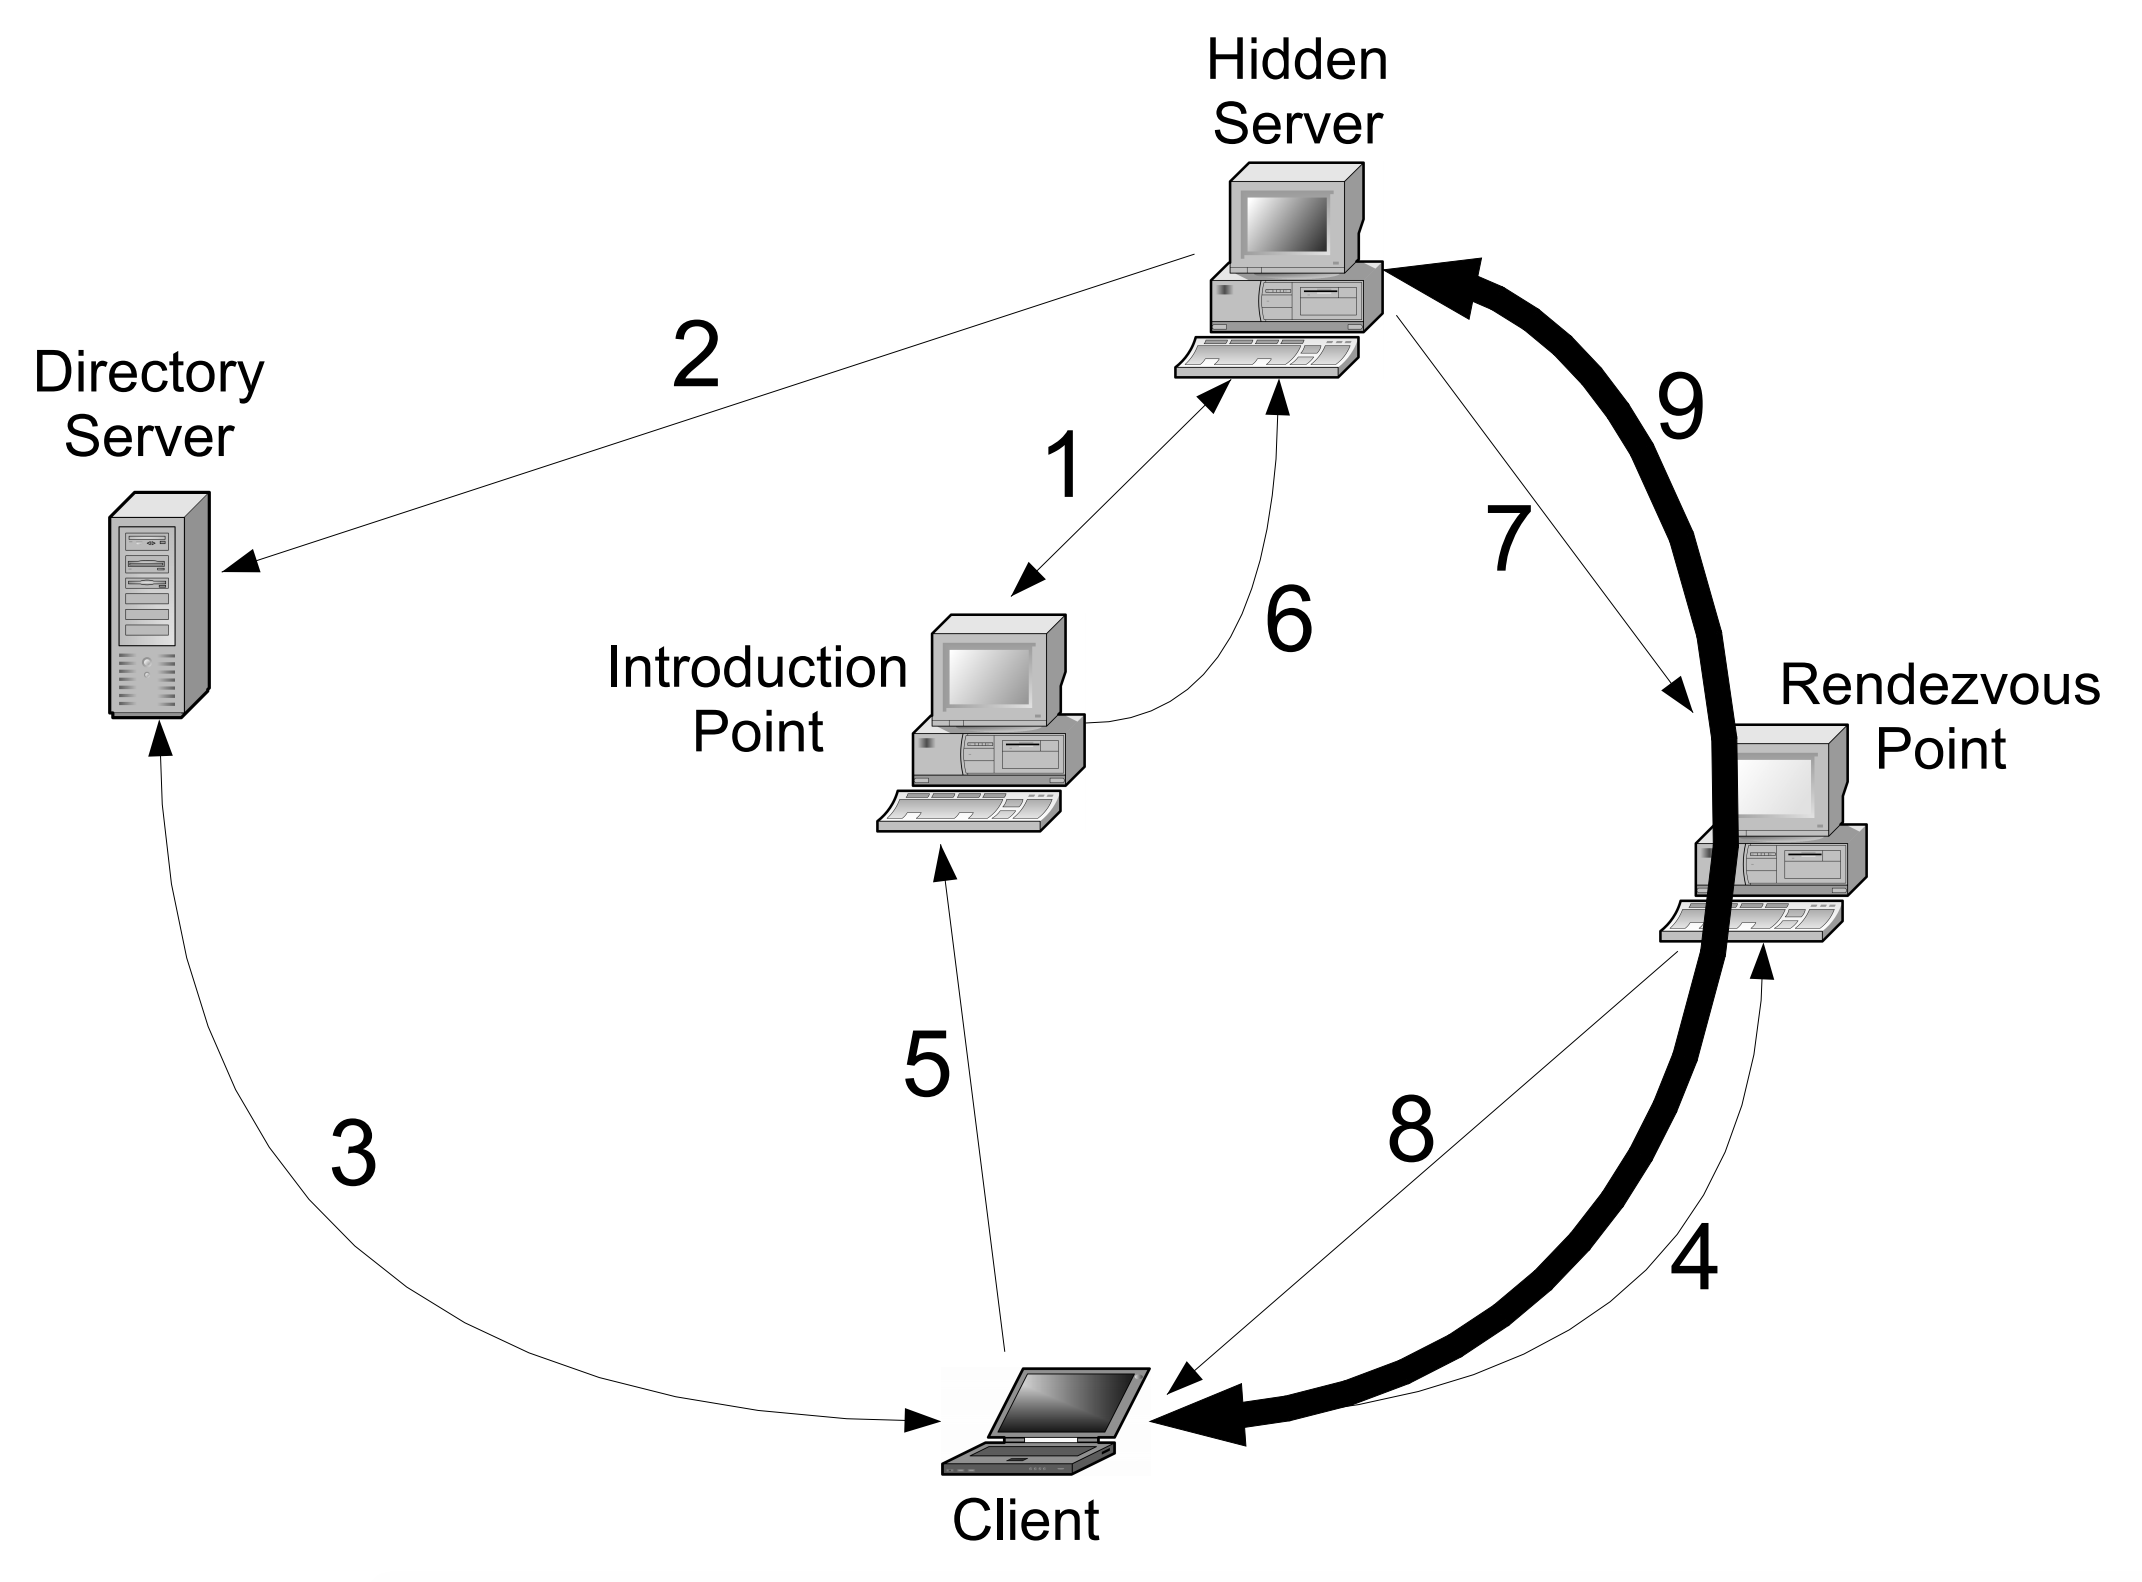
\includegraphics[scale=0.24]{figures/onion-routing.png}
}

\vskip 0.4in

\noindent First the Hidden Server connects (1) to a node in the Tor network and asks if it is OK for the node to act as an Introduction Point for his service. If the node accepts, we keep the circuit open and continue; otherwise HS tries another node until successful. These connections are kept open forever. Next, the Hidden Server contacts (2) the Directory Server and asks it to publish the contact information of its hidden service. The hidden service is now ready to receive connection requests from clients. In order to retrieve data from the service the Client connects (3) to DS and asks for the contact information of the identified service and retrieves it if it exists (including the addresses of Introduction Points). The Client then selects a node in the network to act as a Rendezvous Point, connects (4) to it and asks it to listen for connections from a hidden service on C's behalf. The Client repeats this until a Rendezvous Point has accepted, and then contacts (5) the Introduction Point and asks it to forward the information about the selected RP. The Introduction Point forwards (6) this message to the Hidden Server who determines whether to connect to the Rendezvous Point or not. If OK, the Hidden Server connects (7) to RP and asks to be connected to the waiting rendezvous circuit, and RP then forwards (8) this connection request to the Client. Now RP can start passing data between the two connections and the result is an anonymous data tunnel (9) from C to HS through RP.

\vskip 0.2in 

\noindent L. {\O}verlier and P. Syverson. ``Locating Hidden Servers.'' \textit{IEEE Symposium on Security and Privacy}, May 2006.


\chapter{LamdaMOO}

{\footnotesize
\ttfamily
\parindent0pt
\parskip6pt
telnet lambda.moo.mud.org 8888

Trying 209.181.94.35...

Connected to lambda.moo.mud.org.

\begin{verbatim}
                ***************************
                *  Welcome to LambdaMOO!  *
                ***************************


           Running Version 1.8.3+47 of LambdaMOO
\end{verbatim}

PLEASE NOTE:

LambdaMOO is a new kind of society, where thousands of people voluntarily
come together from all over the world.  What these people say or do may not
always be to your liking; as when visiting any international city, it is wise
to be careful who you associate with and what you say.

The operators of LambdaMOO have provided the materials for the buildings of
this community, but are not responsible for what is said or done in them.  In
particular, you must assume responsibility if you permit minors or others to
access LambdaMOO through your facilities.  The statements and viewpoints
expressed here are not necessarily those of the wizards, Pavel Curtis,
or Roger Crew, and those parties disclaim any responsibility for them.

For assistance either now or later, type `help'.
The lag is low; there are 64 connected.
connect Guest

*** Connected ***

The Coat Closet

The closet is a dark, cramped space.  It appears  to be very crowded in here; you keep bumping into what feels like coats,  boots, and other people (apparently sleeping).  One useful thing that you've  discovered in your bumbling about is a metal doorknob set at waist level into  what might be a door.  Next to it is a spring lever labeled 'QUIET!'.

There is new news.  Type `news' to read all news or `news new' to read just new news.

Type `@tutorial' for an introduction to basic MOOing.  If you have not already done so, please type `help manners' and read the text carefully.  It outlines the community standard of conduct, which each player is expected to follow while in LambdaMOO.

open door

You open the closet door and leave the darkness for the living room, closing the door behind you so as not to wake the sleeping people inside.

The Living Room

It is very bright, open, and airy here, with large plate-glass windows looking southward over the pool to the gardens beyond.  On the north wall, there is a rough stonework fireplace.  The east and west walls are almost completely covered with large, well-stocked bookcases.  An exit in the northwest corner leads to the kitchen and, in a more northerly direction, to the entrance hall.  The door into the coat closet is at the north end of the east wall, and at the south end is a sliding glass door leading out onto a wooden deck.  There are two sets of couches, one clustered around the fireplace and one with a view out the windows.

You see Welcome Poster, a fireplace, the living room couch, Statue, The Birthday Machine, Helpful Person Finder, lag meter, a map of LambdaHouse, and Cockatoo here.

Tessier (out on his feet), Sage (smitten), Jed (out on his feet), Rusty (distracted), Sleeper (in deep meditation), and Fox-In-Sox (out on his feet) are here.

The cuckoo clock begins making a small whirring noise.

 >~>~Cuckoo!~<~<

You hear a small click coming from the cuckoo clock.

look at statue

A large statue of the Roman Goddess, Minerva. Made of white marble, she stands seven feet tall, chin held high, and draped in long flowing gowns of stone. In her left hand, palm upward, rests a carefully carved tome; in her right, clenched in a stony grip, is a spear.  The artisan who crafted her obviously spent a great deal of time on the eyes: they exude a fierceness expected of the goddess of war, but at the same time, the chiselled stone bleeds that sadness that is borne of wisdom.

She watches over the Living Room with her unending gaze, and, like so many other anthropomorphic oddities on the MOO, gives help when and where she can.  To find out something from Minerva:

Directed speech requests(``to <this thing>''):

news <subject> : News headlines about subject

weather <zipcode> : current weather

whatis <something> : Wikipedia info

summarize <url> : summarize contents of page

For more information regarding `MOORadio', type help \#26270  (Statue of Minerva).

The Statue of Minerva also uses the aliases: helper, min, mini and statue.

north

The Entrance Hall

This small foyer is the hub of the currently-occupied portion of the house.  To the north are the double doors forming the main entrance to the house.  There is a mirror at about head height on the east wall, just to the right of a corridor leading off into the bedroom area.  The south wall is all rough stonework, the back of the living room fireplace; at the west end of the wall is the opening leading south into the living room and southwest into the kitchen.  Finally, to the west is an open archway leading into the dining room.

You see mirror at about head height, a globe, Edgar the Footman, MOO population meter, and an antique suit of armour here.

look at mirror

You look into the mirror and feel yourself being drawn into it, as if gravity had suddenly turned 90 degrees.

Looking Glass Tavern Bar

The bar of the Looking Glass Tavern is one vast, smooth expanse of primeval wood (from the primeval forest) against the north wall, polished to a high sheen by the never-ending efforts of a not-quite-human bartender.  Behind the bar is a mirror that doesn't appear to be reflecting the contents of the room accurately...

Steps lead up, to the second floor and down, to the cellar.  A stack of cases of Old Frothing Slosh beer rest in the southwest corner.

You see drunken stupor, a long mirror that looks kind of hazy and doesn't quite reflect the contents of the room, PacMOO Video Game, a dart board, Kombat Arena II arcade game, Portable Full Length Mirror, Spacewar Video Game, Bottle of Mist, Jake, bar, Bert the Boojum, Bill, and Lou Carol here.

Heliosa (asleep) is here.

You suddenly realize you're somewhere else.

up

You climb up the spiral staircase to the second floor.

Tavern Second Floor

This is the second floor of the Looking Glass Tavern, where rooms are
rented to steady customers on a long-term basis.  There are several doors on
either side of the hallway, some marked vacant, many bearing room numbers and
the names of the occupants.  The hallway extends back to the east, leading
to what appears to be a less-used area.

The spiral staircase leading to the first floor is at the west end of the
 hallway.

Contents:

~ ~plaque titled Directory

read Directory

The following is engraved on the plaque:

~ ~Looking Glass Tavern Room Directory

Beginning exit transfer thingie run, invoked by player Fawn\_Guest (\#92111)

\begin{verbatim}
Room 06, Legion  Room 10, Hookleg     Room 12, Xatrix
Room 13, antox   Room 16, ring        Room 48, Violetta
Room 60, Anxis   Room 69, Wintermute  Room 93, Hookleg
\end{verbatim}

Space is available.  Please feel free to add a room for yourself.
Please do not use compass directions for exit names from the hallway.
Please use some two-digit number as the NAME of the exit.
Please use @add-entrance and @add-exit to link in.  This room is link\_ok.
Oh yes... please remember to put OARRIVES and OLEAVES on your exit.

- The Mgt.

The following door numbers are available:

00, 01, 02, 03, 04, 05, 07, 08, 09, 11, 14, 15, 17, 18, 19, 20, 21, 22, 23, 24, 25, 26, 27, 28, 29, 30, 31, 32, 33, 34, 35, 36, 37, 38, 39, 40, 41, 42, 43, 44, 45, 46, 47, 49, 50, 51, 52, 53, 54, 55, 56, 57, 58, 59, 61, 62, 63, 64, 65, 66, 67, 68, 70, 71, 72, 73, 74, 75, 76, 77, 78, 79, 80, 81, 82, 83, 84, 85, 86, 87, 88, 89, 90, 91, 92, 94, 95, 96, 97, 98, and 99

down

look at long mirror

north

You open the front door and walk outside.

Driveway

A circular driveway, in front of LambdaHouse. The LambdaHouse front door is to
 the south. The drive curves away to the northeast and northwest.

You see springboard, Information Center, a copy of the MidNite-MOO, Foodmart shopping cart, and a brand new shiny penny here.

You carefully shut the door behind you.

take penny

You take a brand new shiny penny.

look at penny

A brand new shiny copper penny, with the words "For your thoughts" engraved on
 both sides.

northeast

You wander out toward the street.

Street in front of LambdaHouse

A quiet east-west street that runs in front of LambdaHouse. There's a large
 tree, with a white painted trunk, in the middle of the road.  On the south
 side of the street, a manhole leads down. There is a rope ladder here which
 leads up into a cardboard box at the top of the tree.

You see Road Construction Warning Sign here.

down

You lift the manhole cover and climb down, closing the manhole behind
 yourself.  You climb a rusty metal ladder down into a sewage pipe and land in
 a stink of sludge.

Sewage pipe

This is a large east-west sewage pipe.  Debris from a recent earthquake blocks
 the west passageway.  Roots from a large tree have pentrated the pipe from
 the north and have spread out to the west.  A small passage to the north has
 been hacked from the mass of roots.  Sticky sludge sucks at your feet.  There
 is some graffiti reading ``Monday, March 24, 1997  Control of the thumb
 requires more of the brain's gray matter than does the control of the chest
 and abdomen.'' scrawled on the interior of the pipe.  A smaller pipe drains
 into this one from the south.  A rusty ladder leads up.

south

You step into the smaller pipe to the south, your feet squishing in the sludge.
Sewage pipe

This is a north-south sewage pipe.  Sticky sludge sucks at your feet.  This
 pipe drains into a larger east-west pipe to the north.  There is a lot of
 graffiti on the interior of the pipe.  The first of it reads: A.Word.A.Day
 -lollygag.  You could read the rest of it, if you want to read dozens of
 lines.

south

You go south, your feet squishing in the sludge.

Sewage pipe

This is a north-south sewage pipe.  The passage south is blocked by a rusty
 grille.  Sticky sludge sucks at your feet.  There is some graffiti reading
 ``XRX: Last 116 \&nbsp; 1/8 High 117 \&nbsp; 5/8 Low 115 \&nbsp; 13/16 Volume
 1,246,600 Div \$0.36 As of  2:15 PM EST on Jan 19 Change - \&nbsp; 1/4
 \&nbsp;0.21\% YearHigh 123.37 YearLow 71.25 P/E 168 Yield 1.24\% Exchange NYSE''
 scrawled on the interior of the pipe.  A tunnel with rungs leading up is
 above.
 
up

You climb up the tunnel and reach the grating.  You push the grating aside and
 climb into a cramped space.  The grating clangs back into place.

Underneath the desk

It's the space below the desk.  It's even more cramped than the office.  Lots
 of junk, apparently spilled from the desk, clutter this area.  When you're
 through looking around here, you can exit to the office, or you can explore
 the grating on the floor.

You see IRC cable, hypodermic needle, LambdaMOO hallucinogen, and JaysHouseMOO hallucinogen here.

exit

You leave for the (relative) spaciousness of the office.

Messy, cramped office

This room is cramped and cluttered, and clearly unsafe.  A bare light bulb
 hangs down from between the pipes and ducts on the ceiling.  The concrete
 walls are slightly damp and covered with a thin layer of mold.  The
 ventilation is almost nonexistent, and the southern door leading to the rest
 of the basement is half-blocked by the desk.  At the desk, qpliu is asleep,
 his head planted on the keyboard in front of him.  The desk occupies most of
 the floorspace.  On the desk is a cheap BW X terminal surrounded by empty
 coke cans, and pile of printouts and photocopied papers.  On the back part of
 the desk, a book\-case sags under the weight of old textbooks.  A muddy\\
 bicycle is leaning against the bookcase, making a mess of \\ the papers beneath is, as well as making most of the desk \\ unusable.  In addition, Revolving Door Maze,
 Room with dy\-namic graffiti, Revolving Door Maze, Revolving Door Maze, \\
 Revolving Door Maze, Revolving Door Maze, Revolving Door \\ Maze, Revolving Door
 Maze, Revolving Door Maze, Revolving \\ Door Maze, Revolving Door Maze,
 Revolving Door Maze, \\ Revolving Door Maze, Revolving Door Maze, Revolving Door \\
 Maze, Revolving Door Maze, Revolving Door Maze, Sewage \\ pipe, Sewage pipe,
 Sewage pipe, and generic multichannel \\ IRC headphones are on the desk.  There
 is a little space \\ underneath the desk.  You probably could crawl there.

You see a red wagon (carrying picture of Scutmonkey), simple IRC headphones, and multichannel IRC headphones here.

qpliu (asleep) is here.

out

The door bangs into the desk as you open it, leaving only a narrow crack.  You
 manage to sqeeze through, though.

Basement

It's a basement. A fireproof door of steel-reinforced construction is to the
 east. There is a banged up door in the north wall.  There is a rat-sized hole
 in the southern wall.  Furnace is sitting in here.  About 4 feet up on the
 west wall is a board with a hinge at the top.

You see thermostat and tool box here.

west

You pull the board towards you and crawl up into the hole in the wall.

Crawl Space

A dark cramped space no more than five feet high.  Joists run overhead
 supporting the floor under the Family Room and Kitchen; underneath is bare
 dirt.  The sound of humming machinery can be heard to the east.  You feel the
 draft of a door to the west.

It takes a moment for your eyes to adjust to the darkness.

west

You push aside the crawlspace door and hop down onto the basement landing.

Basement Landing

The iron spiral staircase heads up into the light, and down, but you can only
 see darkness below.  Four feet up from the landing on the east wall is an
 entrance to the crawl space under the Family Room.

up

The Family Room

It is comfortably crowded here with plush couches and easy chairs, several
 large bookcases and a free-standing round fireplace.  To the east is the
 kitchen.  There is a doorway leading to the north and a sliding glass door to
 the south, through which you can see the gardens.  In the southwest corner of
 the room is an ironwork spiral staircase leading up and down.  A plywood
 board used to block downward access, but some vandal has ripped it off the
 staircase.

You see a display case hanging on the wall, bookcase, a toy box, a postcard from France, couch, VCR/TV, and Weather Map here.

south

The Yard

The yard has ankle-high grass that turns to weeds next to the rosebushes to
 the east, and extends southward a ways toward what appears to be an old
 gazebo.  Off to the west, the yard becomes even less well tended.  To the
 north is a crooked sliding glass door into the house.   Lights from the
 family room light the area.

You see Kilik's Dog House (a light is on inside), a rusty barrel, Kilik's Patented Fireworks Show, The Lawnmower, frisbee, and a bright orange spark here.

You hear soft snoring from inside the doghouse.

west

West of the Yard

Jupiter, Mars, Venus and Mercury join in the southern skies to form a
 fantastic display.

The grounds are slightly better kept to the east. A few trees stand beyond the
 low, split-rail fence which runs along the western border of the property.

You see Chapel here.

look at Chapel

A very large box-shaped wooden structure; it looks large enough that a few
 people could fit inside it. Its richly colored wooden surfaces show off
 intricate carvings. Stained glass windows are set in its sides. There seems
 to be a door you can enter.

enter Chapel

You enter the chapel respectfully.

Chapel

A quiet place with wood panelling. Light filters in from muted stained-glass
 windows. Here you may sit, stand, kneel, prostrate, levitate, pray, meditate,
 shout, whine, flame, chant, cower, pout, contemplate, sigh, confess, float,
 plead, relax, officiate, sermonize, listen, recline, rant, wait, idle, sleep,
 lag, respond, nap, or genuflect as your inclinations dictate.

Chaplain is here.

out

You exit from the chapel with quiet dignity.

West of the Yard

Jupiter, Mars, Venus and Mercury join in the southern skies to form a
 fantastic display.

The grounds are slightly better kept to the east. A few trees stand beyond the
 low, split-rail fence which runs along the western border of the property.

You see Chapel here.

west

Meadow

The eastern end of a vast meadow, where a Gypsy band has built its camp. The
 air is cool and damp and smells of onion grass. Colorful Gypsy wagons are
 scattered in all directions. A light green wagon sits to the Northwest.

Moonlight bathes the meadow in a silvery glow as a chorus of crickets fill the
 damp night air.

An old well sits in the center of this part of the meadow. A soft west breeze
 carries the odors of wood smoke and cooking from the center of camp. An oddly
 smaller wagon stands invitingly open to the southwest. Between two wagons to
 the north, something gleams briefly. A sign on the wagon to the south reads
 `BonJarleycorn.' And east, through some trees and over a low, split-rail
 fence, are the gardens of the main house.

north

Landing Site

A large grassy field to the west of LambdaHouse occasionally utilized as a
 landing site for various aircraft. To the south is a similar field surrounded
 by gypsy caravans, and to the north, the elusive Lambda Street runs by. To
 the east, a small section of driveway bends around from the front of the
 house and goes into the garage.  It is freezing cold out here.  The morning
 sun is easily seen.

You see windsock and helicopter N001LM here.

enter helicopter

You climb into the helicopter.

Helicopter N001LM

You are inside a luxuriously appointed helicopter, just waiting to be flown.
 There seems to be a placard with some basic instructions.
  Through the canopy you see Landing Site.

read instructions

From outside:

look helicopter\\
preflight helicopter\\
enter/board helicopter\\

From inside:

look\\
start\\
hover\\
fly\\
faster\\
slower\\
higher\\
lower\\
look out\\
look down\\
look hobbs\\
look chart\\
scrutinize chart\\
land\\
land <location>\\
overfly <location>\\
wave\\
stop\\
shutdown\\
exit/jump/disem*bark

The helicopter itself can only land at locations that have a wind sock.  You
 can specify where you would like to land:  Type `look chart' to see the
 available locations.  You  *can*  get to the other places you see, but you
 have to jump....

For overflying:  You can only overfly locations that the helicopter knows
 about.  You can specify the location you want to overfly either by its
 number, or by its name in your @rooms database.  To find out what locations
 the helicopter knows about, you have to scrutinize the chart.

Group sky diving:  The best way to sky dive in a group is to pull the
 helicopter into a hover over your chosen destination.  Then everyone who
 jumps will land in the same place.

For detailed technical information about the helicopter, type `notes on
 <helicopter>.

You consult the chart and see that the following locations can accomodate a helicopter:

\begin{verbatim}
#5809     Asphalt Roof
#6295     Airport Helipad
#24641    A Decent Piece of Turf
#66468    Glenrock Station
#58923    Open Field
#19434    Garden
#5468     Landing Site
#88543    Mundania International Heliport (MIH)
#26512    Yib's Helicopter Towing Company
#16043    Treehouse Helipad
#74864    Ski Resort
#9995     Radio KSLP Field
#14077    Zurkian International Runway
#107900   Grassy plateau
#109084   Solitary Glade
#37892    Artic Tundra
#84594    The Eyrie
#68249    Garden
#80723    Inexplicable Meadow
#118284   Grey Stone Roof
\end{verbatim}

start

You follow the checklist and start up the engine.

The roar of the engine is so loud that you can no longer hear what anyone outside is saying.

fly

You start flying the helicopter.

Through the canopy you see The Sky.

As you fly along, you see Glenrock Station.

As you fly along, you see The Deck.

As you fly along, you see Street in front of the Pet Store.

As you fly along, you see Garden.

As you fly along, you see Street in front of LambdaHouse.

land Ski Resort

You land the helicopter.

Through the canopy you see Ski Resort.

out

Please shut down the engine first.

stop

You follow the checklist and shut down the engine.

out

You climb out of the helicopter.

Ski Resort

The snow is at its best for skiing! The runs are well packed and fast. The
 beauty of the panoramic views of snow covered mountains are only rivalled by
 the blue Pacific ocean in the west. The ski lift is taking people up to the
 top of the mountain. Lots of people from all over the world are here skiing,
 sledding and having snowball play fights.
 
You see a Greyhound Bus, Chopper(helicopter), and a Ski Lift here.

Exits: Board->the bus; Lift->top of mountain; Enter->chopper; Walk -> takes you along a path to a peaceful valley in the west.

Everywhere you look there are snow capped mountains reflecting the bright
 moonlight. People are laughing and enjoying the night skiing as the runs are
 lit up too tonight.

You see Wind Sock, Chopper, and helicopter N001LM here.

Lift

As you go higher on the lift you turn as the people are waving and calling,
 good-bye Guest , come on back, okay?

Coastal Mountain Range Public Park

You're on a mountain 1000 meters high with a view of the Pacific Coast
 mountain range and the Pacific ocean in the west. Its cold up here but theres
 a natural hot springs pool and a campfire beside the ledge. The ledge
 shelters the pool from winds and creates an ecology where wild flowers grow
 year round in the steam from the pool. The wind is wonderful for the
 hanggliders here and you're welcome to use them, as well as the guest cabin
 and pool. Park rangers keep the picnic basket(bar) filled with food for
 visitors. This is your park, please don't feed the wildlife.

For directions on the hanggliders type Look Sign. You're welcome to sit in the
 hot springs pool.

Exits: in~->~guest cabin. ski~->~ski ramp. open~->~hole in the ground. down~->~the rainforest.

The moonlight reflects off all the snowcapped mountains and lights a path
 along the ocean in the west.
 
You see a campfire, a hole in the ground, and down here.

You get to the top, jump off the lift and go over to the campfire to warm up.

...
}


\chapter{The Mythical Man-Month (Fred Brooks)}

\begin{quote}
\emph{Good cooking takes time. If you are made to wait, it is to 
serve you better, and to please you.}

\emph{-- Menu of Restaurant Antoine, New Orleans}
\end{quote}

\noindent More software projects have gone awry for lack of calendar time 
than for all other causes combined. Why is this cause of disaster 
so common? 

First, our techniques of estimating are poorly developed. More 
seriously, they reflect an unvoiced assumption which is quite untrue, i.e., that all will go well. 

Second, our estimating techniques fallaciously confuse effort 
with progress, hiding the assumption that men and months are 
interchangeable. 

Third, because we are uncertain of our estimates, software 
managers often lack the courteous stubbornness of Antoine's chef. 

Fourth, schedule progress is poorly monitored. Techniques 
proven and routine in other engineering disciplines are considered 
radical innovations in software engineering. 

Fifth, when schedule slippage is recognized, the natural (and 
traditional) response is to add manpower. Like dousing a fire with 
gasoline, this makes matters worse, much worse. More fire requires more gasoline, and thus begins a regenerative cycle which 
ends in disaster. 

Schedule monitoring will be the subject of a separate essay. 
Let us consider other aspects of the problem in more detail. 

\section{Optimism}

All programmers are optimists. Perhaps this modern sorcery especially attracts those who believe in happy endings and fairy godmothers. Perhaps the hundreds of nitty frustrations drive away all 
but those who habitually focus on the end goal. Perhaps it is 
merely that computers are young, programmers are younger, and 
the young are always optimists. But however the selection process 
works, the result is indisputable: ``This time it will surely run,'' or 
``I just found the last bug.''

So the first false assumption that underlies the scheduling of 
systems programming is that \emph{all will go well}, i.e., that \emph{each task will 
take only as long as it ``ought'' to take.}

The pervasiveness of optimism among programmers deserves 
more than a flip analysis. Dorothy Sayers, in her excellent book, 
\emph{The Mind of the Maker}, divides creative activity into three stages: 
the idea, the implementation, and the interaction. A book, then, 
or a computer, or a program comes into existence first as an ideal 
construct, built outside time and space, but complete in the mind 
of the author. It is realized in time and space, by pen, ink, and 
paper, or by wire, silicon, and ferrite. The creation is complete 
when someone reads the book, uses the computer, or runs the 
program, thereby interacting with the mind of the maker. 

This description, which Miss Sayers uses to illuminate not 
only human creative activity but also the Christian doctrine of the 
Trinity, will help us in our present task. For the human makers of 
things, the incompletenesses and inconsistencies of our ideas, 
become clear only during implementation. Thus it is that writing, 
experimentation, ``working out'' are essential disciplines for the 
theoretician. 

In many creative activities the medium of execution is intractable. Lumber splits; paints smear; electrical circuits ring. These 
physical limitations of the medium constrain the ideas that may 
be expressed, and they also create unexpected difficulties in the 
implementation. 

Implementation, then, takes time and sweat both because of 
the physical media and because of the inadequacies of the underlying ideas. We tend to blame the physical media for most of our 
implementation difficulties; for the media are not ``ours'' in the 
way the ideas are, and our pride colors our judgment. 

Computer programming, however, creates with an exceedingly tractable medium. The programmer builds from pure 
thought-stuff: concepts and very flexible representations thereof. 
Because the medium is tractable, we expect few difficulties in 
implementation; hence our pervasive optimism. Because our ideas 
are faulty, we have bugs; hence our optimism is unjustified. 

In a single task, the assumption that all will go well has a 
probabilistic effect on the schedule. It might indeed go as planned, 
for there is a probability distribution for the delay that will be 
encountered, and ``no delay" has a finite probability. A large programming effort, however, consists of many tasks, some chained 
end-to-end. The probability that each will go well becomes vanishingly small. 

\section{The Man-Month}

The second fallacious thought mode is expressed in the very unit 
of effort used in estimating and scheduling: the man-month. Cost 
does indeed vary as the product of the number of men and the 
number of months. Progress does not. \emph{Hence the man-month as a unit 
for measuring the size of a job is a dangerous and deceptive myth.} It 
implies that men and months are interchangeable.

Men and months are interchangeable commodities only when 
a task can be partitioned among many workers \emph{with no communication among them} (Fig.~\ref{fig:mmm-2-1}). This is true of reaping wheat or picking 
cotton; it is not even approximately true of systems programming. 

\begin{figure}[h]
\centering
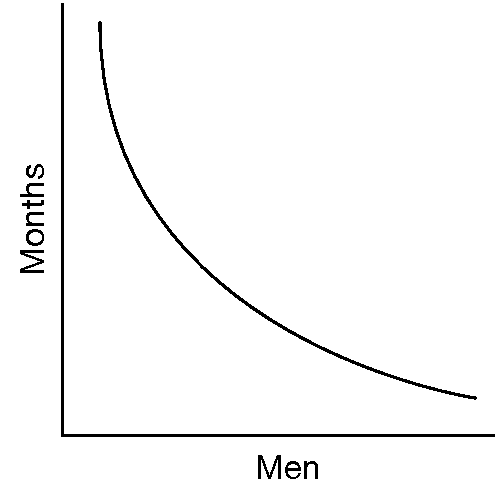
\includegraphics[scale=0.65]{figures/mythical-man-month-fig-2-1.pdf}
\caption{Time versus number of workers -- perfectly partitionable task}
\label{fig:mmm-2-1}
\end{figure}

When a task cannot be partitioned because of sequential constraints, the application of more effort has no effect on the schedule (Fig.~\ref{fig:mmm-2-2}). The bearing of a child takes nine months, no matter 
how many women are assigned. Many software tasks have this 
characteristic because of the sequential nature of debugging. 

\begin{figure}[h]
\centering
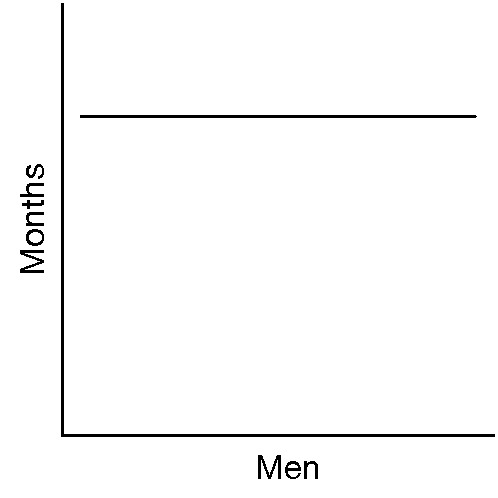
\includegraphics[scale=0.65]{figures/mythical-man-month-fig-2-2.pdf}
\caption{Time versus number of workers -- unpartitionable task}
\label{fig:mmm-2-2}
\end{figure}

In tasks that can be partitioned but which require communication among the subtasks, the effort of communication must be 
added to the amount of work to be done. Therefore the best that 
can be done is somewhat poorer than an even trade of men for 
months (Fig.~\ref{fig:mmm-2-3}). 

\begin{figure}[h]
\centering
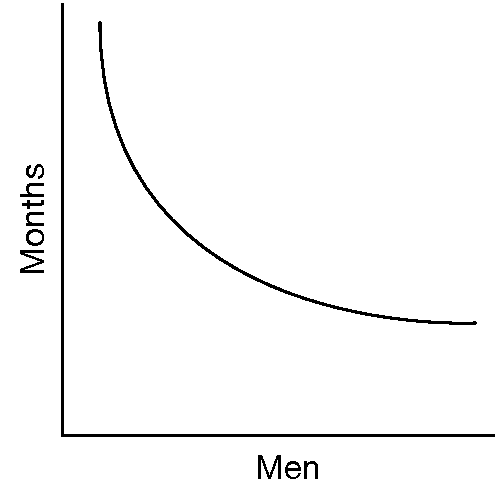
\includegraphics[scale=0.65]{figures/mythical-man-month-fig-2-3.pdf}
\caption{Time versus number of workers -- partitionable task requiring communication}
\label{fig:mmm-2-3}
\end{figure}


The added burden of communication is made up of two parts, 
training and intercommunication. Each worker must be trained in 
the technology, the goals of the effort, the overall strategy, and the 
plan of work. This training cannot be partitioned, so this part of 
the added effort varies linearly with the number of workers.

Intercommunication is worse. If each part of the task must be 
separately coordinated with each other part, the effort increases as 
$n(n-1)/2$. Three workers require three times as much pairwise 
intercommunication as two; four require six times as much as two. 
If, moreover, there need to be conferences among three, four, etc., 
workers to resolve things jointly, matters get worse yet. The added 
effort of communicating may fully counteract the division of the 
original task and bring us to the situation of Fig.~\ref{fig:mmm-2-4}. 

\begin{figure}[h]
\centering
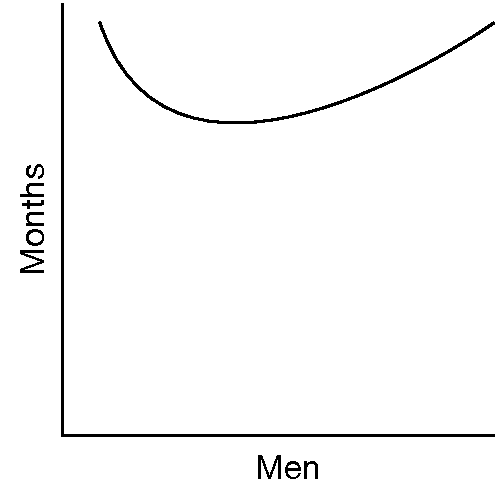
\includegraphics[scale=0.65]{figures/mythical-man-month-fig-2-4.pdf}
\caption{Time versus number of workers -- task with complex interrelationships}
\label{fig:mmm-2-4}
\end{figure}

Since software construction is inherently a systems effort -- an 
exercise in complex interrelationships -- communication effort is 
great, and it quickly dominates the decrease in individual task time 
brought about by partitioning. Adding more men then lengthens, 
not shortens, the schedule. 

\section{Systems Test}

No parts of the schedule are so thoroughly affected by sequential 
constraints as component debugging and system test. Furthermore, the time required depends on the number and subtlety of 
the errors encountered. Theoretically this number should be zero. 
Because of optimism, we usually expect the number of bugs to be 
smaller than it turns out to be. Therefore testing is usually the 
most mis-scheduled part of programming. 

For some years I have been successfully using the following 
rule of thumb for scheduling a software task: 

\begin{itemize}
\item[] \nicefrac{1}{3} planning 
\item[] \nicefrac{1}{6} coding 
\item[] \nicefrac{1}{4} component test and early system test 
\item[] \nicefrac{1}{4} system test, all components in hand. 
\end{itemize}

This differs from conventional scheduling in several important 
ways: 

\begin{enumerate}
\item The fraction devoted to planning is larger than normal. Even 
so, it is barely enough to produce a detailed and solid specification, and not enough to include research or exploration of 
totally new techniques. 

\item The \emph{half} of the schedule devoted to debugging of completed 
code is much larger than normal. 

\item The part that is easy to estimate, i.e., coding, is given only 
one-sixth of the schedule. 
\end{enumerate}

In examining conventionally scheduled projects, I have found 
that few allowed one-half of the projected schedule for testing, 
but that most did indeed spend half of the actual schedule for that 
purpose. Many of these were on schedule until and except in 
system testing.

Failure to allow enough time for system test, in particular, is 
peculiarly disastrous. Since the delay comes at the end of the 
schedule, no one is aware of schedule trouble until almost the 
delivery date. Bad news, late and without warning, is unsettling 
to customers and to managers. 

Furthermore, delay at this point has unusually severe financial, as well as psychological, repercussions. The project is fully 
staffed, and cost-per-day is maximum. More seriously, the software is to support other business effort (shipping of computers, 
operation of new facilities, etc.) and the secondary costs of delaying these are very high, for it is almost time for software shipment. Indeed, these secondary costs may far outweigh all others. It is 
therefore very important to allow enough system test time in the 
original schedule. 

\section{Gutless Estimating}

Observe that for the programmer, as for the chef, the urgency of 
the patron may govern the scheduled completion of the task, but 
it cannot govern the actual completion. An omelette, promised in 
two minutes, may appear to be progressing nicely. But when it has 
not set in two minutes, the customer has two choices -- wait or eat 
it raw. Software customers have had the same choices. 

The cook has another choice; he can turn up the heat. The 
result is often an omelette nothing can save -- burned in one part, 
raw in another. 

Now I do not think software managers have less inherent 
courage and firmness than chefs, nor than other engineering managers. But false scheduling to match the patron's desired date is 
much more common in our discipline than elsewhere in engineering. It is very difficult to make a vigorous, plausible, and job-risking defense of an estimate that is derived by no quantitative 
method, supported by little data, and certified chiefly by the 
hunches of the managers. 

Clearly two solutions are needed. We need to develop and 
publicize productivity figures, bug-incidence figures, estimating 
rules, and so on. The whole profession can only profit from sharing 
such data. 

Until estimating is on a sounder basis, individual managers 
will need to stiffen their backbones and defend their estimates 
with the assurance that their poor hunches are better than wish-derived estimates. 

\section{Regenerative Schedule Disaster}

What does one do when an essential software project is behind 
schedule? Add manpower, naturally. As Figs.~\ref{fig:mmm-2-1} through~\ref{fig:mmm-2-4} suggest, this may or may not help. 

Let us consider an example. Suppose a task is estimated at 12 
man-months and assigned to three men for four months, and that 
there are measurable mileposts A, B, C, D, which are scheduled to 
fall at the end of each month (Fig.~\ref{fig:mmm-2-5}).


Now suppose the first milepost is not reached until two 
months have elapsed (Fig.~\ref{fig:mmm-2-6}). What are the alternatives facing 
the manager?



\begin{enumerate}
\item Assume that the task must be done on time. Assume that only 
the first part of the task was misestimated, so Fig.~\ref{fig:mmm-2-6} tells the 
story accurately. Then 9 man-months of effort remain, and 
two months, so 4 \nicefrac{1}{2} men will be needed. Add 2 men to the 3 
assigned. 

\item Assume that the task must be done on time. Assume that the 
whole estimate was uniformly low, so that Fig.~\ref{fig:mmm-2-7} really 
describes the situation. Then 18 man-months of effort remain, 
and two months, so 9 men will be needed. Add 6 men to the 
3 assigned. 

\item Reschedule. I like the advice given by P. Fagg, an experienced 
hardware engineer, ``Take no small slips'' That is, allow 
enough time in the new schedule to ensure that the work can 
be carefully and thoroughly done, and that rescheduling will 
not have to be done again. 

\item Trim the task. In practice this tends to happen anyway, once 
the team observes schedule slippage. Where the secondary 
costs of delay are very high, this is the only feasible action. 
The manager's only alternatives are to trim it formally and 
carefully, to reschedule, or to watch the task get silently 
trimmed by hasty design and incomplete testing. 

\end{enumerate}

\begin{figure}[h]
\centering
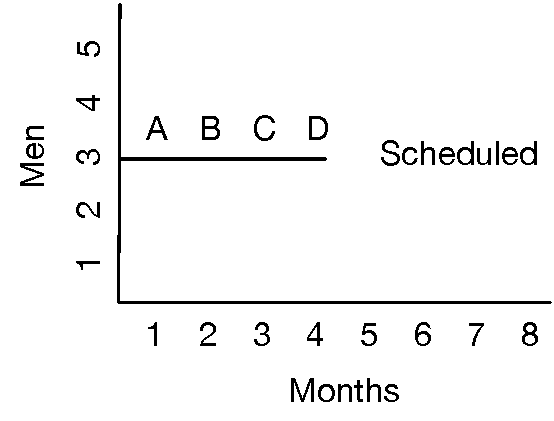
\includegraphics[scale=0.65]{figures/mythical-man-month-fig-2-5.pdf}
\caption{}
\label{fig:mmm-2-5}
\end{figure}

\begin{figure}[h]
\centering
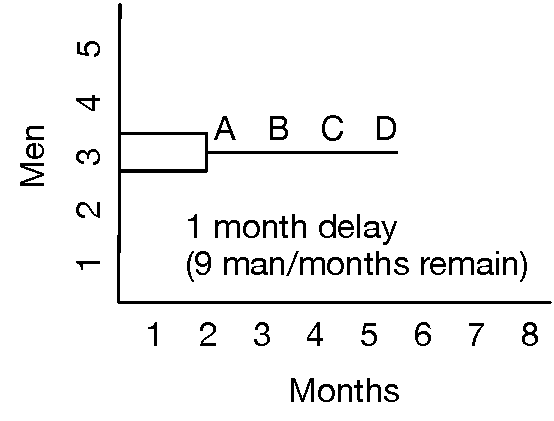
\includegraphics[scale=0.65]{figures/mythical-man-month-fig-2-6.pdf}
\caption{}
\label{fig:mmm-2-6}
\end{figure}

\begin{figure}[h]
\centering
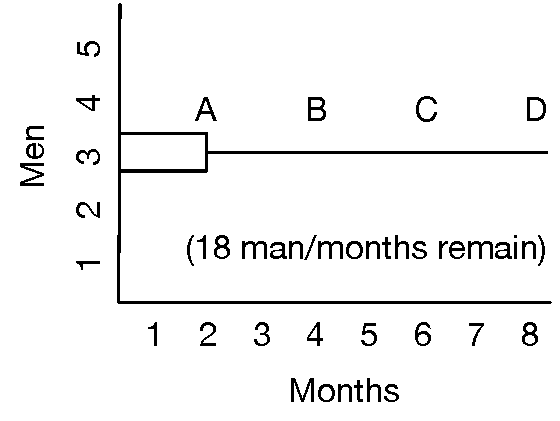
\includegraphics[scale=0.65]{figures/mythical-man-month-fig-2-7.pdf}
\caption{}
\label{fig:mmm-2-7}
\end{figure}

\begin{figure}[h]
\centering
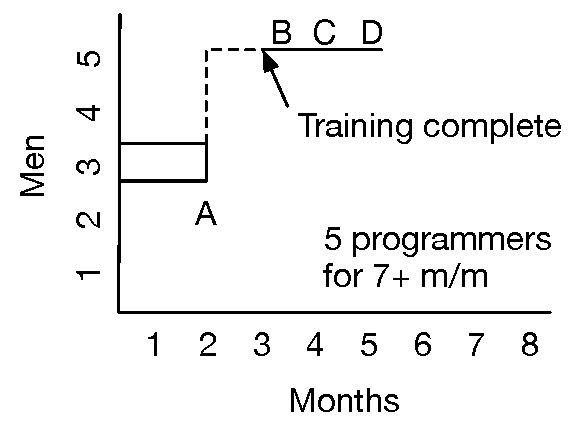
\includegraphics[scale=0.65]{figures/mythical-man-month-fig-2-8.pdf}
\caption{}
\label{fig:mmm-2-8}
\end{figure}

In the first two cases, insisting that the unaltered task be 
completed in four months is disastrous. Consider the regenerative 
effects, for example, for the first alternative (Fig.~\ref{fig:mmm-2-8}). The two new 
men, however competent and however quickly recruited, will require training in the task by one of the experienced men. If this 
takes a month, \emph{3 man-months will have been devoted to work not in the 
original estimate}. Furthermore, the task, originally partitioned three 
ways, must be repartitioned into five parts; hence some work 
already done will be lost, and system testing must be lengthened. 
So at the end of the third month, substantially more than 7 man-months of effort remain, and 5 trained people and one month are 
available. As Fig.~\ref{fig:mmm-2-8} suggests, the product is just as late as if no 
one had been added (Fig.~\ref{fig:mmm-2-6}).

To hope to get done in four months, considering only training 
time and not repartitioning and extra systems test, would require 
adding 4 men, not 2, at the end of the second month. To cover 
repartitioning and system test effects, one would have to add still 
other men. Now, however, one has at least a 7-man team, not a 
3-man one; thus such aspects as team organization and task division are different in kind, not merely in degree. 

Notice that by the end of the third month things look very 
black. The March 1 milestone has not been reached in spite of all 
the managerial effort. The temptation is very strong to repeat the 
cycle, adding yet more manpower. Therein lies madness. 

The foregoing assumed that only the first milestone was 
misestimated. If on March 1 one makes the conservative assumption that the whole schedule was optimistic, as Fig.~\ref{fig:mmm-2-7} depicts, one 
wants to add 6 men just to the original task. Calculation of the 
training, repartitioning, system testing effects is left as an exercise 
for the reader. Without a doubt, the regenerative disaster will 
yield a poorer product, later, than would rescheduling with the 
original three men, unaugmented. 

Oversimplifying outrageously, we state Brooks's Law: 

\begin{quote}
\textbf{Adding manpower to a late software project makes it later.}
\end{quote}

This then is the demythologizing of the man-month. The 
number of months of a project depends upon its sequential constraints. The maximum number of men depends upon the number 
of independent subtasks. From these two quantities one can derive 
schedules using fewer men and more months. (The only risk is 
product obsolescence.) One cannot, however, get workable schedules using more men and fewer months. More software projects 
have gone awry for lack of calendar time than for all other causes 
combined. 



\chapter{Manifesto for Agile Software Development}

We are uncovering better ways of developing software by doing it and helping others do it. Through this work we have come to value:

\begin{itemize}
\item \textbf{Individuals and interactions} over processes and tools
\item \textbf{Working software} over comprehensive documentation
\item \textbf{Customer collaboration} over contract negotiation
\item \textbf{Responding to change} over following a plan
\end{itemize}
That is, while there is value in the items on
the right, we value the items on the left more.

\begin{verse}
\poemtitle{Principles behind the Agile Manifesto}
\emph{We follow these principles:}

Our highest priority is to satisfy the customer \\
through early and continuous delivery \\
of valuable software.

Welcome changing requirements, even late in \\
development. Agile processes harness change for \\
the customer's competitive advantage.

Deliver working software frequently, from a \\
couple of weeks to a couple of months, with a \\
preference to the shorter timescale.

Business people and developers must work \\
together daily throughout the project.

Build projects around motivated individuals. \\
Give them the environment and support they need, \\
and trust them to get the job done.

The most efficient and effective method of \\
conveying information to and within a development \\
team is face-to-face conversation.

Working software is the primary measure of progress.

Agile processes promote sustainable development. \\
The sponsors, developers, and users should be able \\
to maintain a constant pace indefinitely.

Continuous attention to technical excellence \\
and good design enhances agility.

Simplicity--the art of maximizing the amount \\
of work not done--is essential.

The best architectures, requirements, and designs \\
emerge from self-organizing teams.

At regular intervals, the team reflects on how \\
to become more effective, then tunes and adjusts \\
its behavior accordingly.  
\end{verse}




\chapter{The Story of Mel}

This was posted to Usenet by its author, Ed Nather (<nather@astro.as.utexas.edu>), on May 21, 1983.

\vskip 0.2in

\noindent A recent article devoted to the macho side of programming
made the bald and unvarnished statement:
\begin{center}
Real Programmers write in FORTRAN.  
\end{center}

\vskip 0.2in

{\small
\begin{verse}
Maybe they do now, \\
in this decadent era of \\
Lite beer, hand calculators, and ``user-friendly'' software \\
but back in the Good Old Days, \\
when the term ``software'' sounded funny \\
and Real Computers were made out of drums and vacuum tubes, \\
Real Programmers wrote in machine code. \\
Not FORTRAN.  Not RATFOR.  Not, even, assembly language. \\
Machine Code. \\
Raw, unadorned, inscrutable hexadecimal numbers. \\
Directly.

Lest a whole new generation of programmers \\
grow up in ignorance of this glorious past, \\
I feel duty-bound to describe, \\
as best I can through the generation gap, \\
how a Real Programmer wrote code. \\
I'll call him Mel, \\
because that was his name.

I first met Mel when I went to work for Royal McBee Computer Corp., \\
a now-defunct subsidiary of the typewriter company. \\
The firm manufactured the LGP-30, \\
a small, cheap (by the standards of the day) \\
drum-memory computer, \\
and had just started to manufacture \\
the RPC-4000, a much-improved, \\
bigger, better, faster -- drum-memory computer. \\
Cores cost too much, \\
and weren't here to stay, anyway. \\
(That's why you haven't heard of the company, \\
or the computer.)

I had been hired to write a FORTRAN compiler \\
for this new marvel and Mel was my guide to its wonders. \\
Mel didn't approve of compilers.

``If a program can't rewrite its own code'', \\
he asked, ``what good is it?''

Mel had written, \\
in hexadecimal, \\
the most popular computer program the company owned. \\
It ran on the LGP-30 \\
and played blackjack with potential customers \\
at computer shows. \\
Its effect was always dramatic. \\
The LGP-30 booth was packed at every show, \\
and the IBM salesmen stood around \\
talking to each other. \\
Whether or not this actually sold computers \\
was a question we never discussed.

Mel's job was to re-write \\
the blackjack program for the RPC-4000. \\
(Port?  What does that mean?) \\
The new computer had a one-plus-one \\
addressing scheme, \\
in which each machine instruction, \\
in addition to the operation code \\
and the address of the needed operand, \\
had a second address that indicated where, on the revolving drum, \\
the next instruction was located.

In modern parlance, \\
every single instruction was followed by a GO TO! \\
Put that in Pascal's pipe and smoke it.

Mel loved the RPC-4000 \\
because he could optimize his code: \\
that is, locate instructions on the drum \\
so that just as one finished its job, \\
the next would be just arriving at the ``read head'' \\
and available for immediate execution. \\
There was a program to do that job, \\
an ``optimizing assembler'', \\
but Mel refused to use it.

``You never know where it's going to put things'', \\
he explained, ``so you'd have to use separate constants''.

It was a long time before I understood that remark. \\
Since Mel knew the numerical value \\
of every operation code, \\
and assigned his own drum addresses, \\
every instruction he wrote could also be considered \\
a numerical constant. \\
He could pick up an earlier ``add'' instruction, say, \\
and multiply by it, \\
if it had the right numeric value. \\
His code was not easy for someone else to modify.

I compared Mel's hand-optimized programs \\
with the same code massaged by the optimizing assembler program, \\
and Mel's always ran faster. \\
That was because the ``top-down'' method of program design \\
hadn't been invented yet, \\
and Mel wouldn't have used it anyway. \\
He wrote the innermost parts of his program loops first, \\
so they would get first choice \\
of the optimum address locations on the drum. \\
The optimizing assembler wasn't smart enough to do it that way.

Mel never wrote time-delay loops, either, \\
even when the balky Flexowriter \\
required a delay between output characters to work right. \\
He just located instructions on the drum \\
so each successive one was just past the read head \\
when it was needed; \\
the drum had to execute another complete revolution \\
to find the next instruction. \\
He coined an unforgettable term for this procedure. \\
Although ``optimum'' is an absolute term, \\
like ``unique'', it became common verbal practice \\
to make it relative: \\
``not quite optimum'' or ``less optimum'' \\
or ``not very optimum''. \\
Mel called the maximum time-delay locations \\
the ``most pessimum''.

After he finished the blackjack program \\
and got it to run \\
(``Even the initializer is optimized'', \\
he said proudly), \\
he got a Change Request from the sales department. \\
The program used an elegant (optimized) \\
random number generator \\
to shuffle the ``cards'' and deal from the ``deck'', \\
and some of the salesmen felt it was too fair, \\
since sometimes the customers lost. \\
They wanted Mel to modify the program \\
so, at the setting of a sense switch on the console, \\
they could change the odds and let the customer win.

Mel balked. \\
He felt this was patently dishonest, \\
which it was, \\
and that it impinged on his personal integrity as a programmer, \\
which it did, \\
so he refused to do it. \\
The Head Salesman talked to Mel, \\
as did the Big Boss and, at the boss's urging, \\
a few Fellow Programmers. \\
Mel finally gave in and wrote the code, \\
but he got the test backwards, \\
and, when the sense switch was turned on, \\
the program would cheat, winning every time. \\
Mel was delighted with this, \\
claiming his subconscious was uncontrollably ethical, \\
and adamantly refused to fix it.

After Mel had left the company for greener pa\$ture\$, \\
the Big Boss asked me to look at the code \\
and see if I could find the test and reverse it. \\
Somewhat reluctantly, I agreed to look. \\
Tracking Mel's code was a real adventure.

I have often felt that programming is an art form, \\
whose real value can only be appreciated \\
by another versed in the same arcane art; \\
there are lovely gems and brilliant coups \\
hidden from human view and admiration, sometimes forever, \\
by the very nature of the process. \\
You can learn a lot about an individual \\
just by reading through his code, \\
even in hexadecimal. \\
Mel was, I think, an unsung genius.

Perhaps my greatest shock came \\
when I found an innocent loop that had no test in it. \\
No test.  None. \\
Common sense said it had to be a closed loop, \\
where the program would circle, forever, endlessly. \\
Program control passed right through it, however, \\
and safely out the other side. \\
It took me two weeks to figure it out.

The RPC-4000 computer had a really modern facility \\
called an index register. \\
It allowed the programmer to write a program loop \\
that used an indexed instruction inside; \\
each time through, \\
the number in the index register \\
was added to the address of that instruction, \\
so it would refer \\
to the next datum in a series. \\
He had only to increment the index register \\
each time through. \\
Mel never used it.

Instead, he would pull the instruction into a machine register, \\
add one to its address, \\
and store it back. \\
He would then execute the modified instruction \\
right from the register. \\
The loop was written so this additional execution time \\
was taken into account -- \\
just as this instruction finished, \\
the next one was right under the drum's read head, \\
ready to go. \\
But the loop had no test in it.

The vital clue came when I noticed \\
the index register bit, \\
the bit that lay between the address \\
and the operation code in the instruction word, \\
was turned on -- \\
yet Mel never used the index register, \\
leaving it zero all the time. \\
When the light went on it nearly blinded me.

He had located the data he was working on \\
near the top of memory -- \\
the largest locations the instructions could address -- \\
so, after the last datum was handled, \\
incrementing the instruction address \\
would make it overflow. \\
The carry would add one to the \\
operation code, changing it to the next one in the instruction set: \\
a jump instruction. \\
Sure enough, the next program instruction was \\
in address location zero, \\
and the program went happily on its way.

I haven't kept in touch with Mel, \\
so I don't know if he ever gave in to the flood of \\
change that has washed over programming techniques \\
since those long-gone days. \\
I like to think he didn't. \\
In any event, \\
I was impressed enough that I quit looking for the \\
offending test, \\
telling the Big Boss I couldn't find it. \\
He didn't seem surprised.

When I left the company, \\
the blackjack program would still cheat \\
if you turned on the right sense switch, \\
and I think that's how it should be. \\
I didn't feel comfortable \\
hacking up the code of a Real Programmer.
\end{verse}
}

\vskip 0.4in

[1992 postscript -- the author writes: ``The original submission to the net was not in free verse, nor any approximation to it -- it was straight prose style, in non-justified paragraphs. In bouncing around the net it apparently got modified into the `free verse' form now popular. In other words, it got hacked on the net. That seems appropriate, somehow.'' The author adds that he likes the `free-verse' version better than his prose original\dots]

[1999 update: Mel's last name is now known. The manual for the LGP-30 refers to ``Mel Kaye of Royal McBee who did the bulk of the programming [...] of the ACT 1 system''.]

[2001: The Royal McBee LPG-30 turns out to have one other claim to fame. It turns out that meteorologist Edward Lorenz was doing weather simulations on an LGP-30 when, in 1961, he discovered the ``Butterfly Effect'' and computational chaos. This seems, somehow, appropriate.]

[2002: A copy of the programming manual for the LGP-30 lives at {\footnotesize \texttt{http://ed-thelen.org/comp-hist/lgp-30-man.html}}]


\chapter{Things Every Hacker Once Knew (Eric Raymond)}

One fine day in January 2017 I was reminded of something I had half-noticed a few times over the previous decade. That is, younger hackers don't know the bit structure of ASCII and the meaning of the odder control characters in it.

This is knowledge every fledgling hacker used to absorb through their pores. It's nobody's fault this changed; the obsolescence of hardware terminals and the near-obsolescence of the RS-232 protocol is what did it. Tools generate culture; sometimes, when a tool becomes obsolete, a bit of cultural commonality quietly evaporates. It can be difficult to notice that this has happened.

This document is a collection of facts about ASCII and related technologies, notably hardware serial terminals and RS-232 and modems. This is lore that was at one time near-universal and is no longer. It's not likely to be directly useful today -- until you trip over some piece of still-functioning technology where it's relevant (like a GPS puck), or it makes sense of some old-fart war story. Even so, it's good to know anyway, for cultural-literacy reasons.

One thing this collection has that tends to be indefinite in the minds of older hackers is \textit{calendar dates}. Those of us who lived through all this tend to have remembered order and dependencies but not exact timing; here, I did the research to pin a lot of that down. I've noticed that people have a tendency to retrospectively back-date the technologies that interest them, so even if you did live through the era it describes you might get a few surprises from reading this.

There are lots of references to Unix in here because I am mainly attempting to educate younger open-source hackers working on Unix-derived systems such as Linux and the BSDs. If those terms mean nothing to you, the rest of this document probably won't either.

\section{Hardware Context}

Nowadays, when two computers talk to each other, it's usually via TCP/IP over some physical layer you seldom need to care much about. And a ``terminal'' is actually a ``terminal emulator,'' a piece of software that manages part of your display and itself speaks TCP/IP.

Before ubiquitous TCP/IP and bit-mapped displays things were very different. For most hackers that transition took place within a few years of 1992 -- perhaps somewhat earlier if you had access to then-expensive workstation hardware.

Before then there were video display terminals -- VDTs for short. In the mid-1970s these had displaced an earlier generation of printing terminals derived from really old technology called a ``teletype,'' which had evolved around 1900 from Victorian telegraph networks. The very earliest versions of Unix in the late 1960s were written for these printing terminals, in particular for the Teletype Model 33 (aka ASR-33); the ``tty'' that shows up in Unix device names was a then-common abbreviation for ``teletype.''

(This is not the only Unix device name that is a fossil from a bygone age. There's also {\texttt /dev/lp} for the system default printer; every hacker once knew that the ``lp'' stood for ``line printer,'' a type of line-at-a-time electromechanical printer associated with mainframe computers of roughly the same vintage as the ASR-33.)

In those pre-Internet days computers didn't talk to each other much, and the way teletypes and terminals talked to computers was a hardware protocol called ``RS-232'' (or, if you're being pedantic, ``EIA RS-232C''). Before USB, when people spoke of a ``serial'' link, they meant RS-232, and sometimes referred to the equipment that spoke it as ``serial terminals.''

RS-232 had a very long service life; it was developed in the early 1960s, not originally for computer use but as a way for teletypewriters to talk to modems. Though it has passed out of general use and is no longer common knowledge, it's not quite dead even today.

I've been simplifying a bit here. There were other things besides RS-232 and serial terminals going on, notably on IBM mainframes. But they've left many fewer traces in current technology and its folklore. This is because the lineage of modern Unix passes back through a now-forgotten hardware category called a ``minicomputer,'' especially minicomputers made by the Digital Equipment Corporation. ASCII, RS-232 and serial terminals were part of the technology cluster around minicomputers -- as was, for that matter, Unix itself.

Minicomputers were wiped out by workstations and workstations by descendants of the IBM PC, but many hackers old enough to remember the minicomputer era (mid-1960s to mid-1980s) tend still to get a bit misty-eyed about the DEC hardware they cut their teeth on.

Often, however, nostalgia obscures how very underpowered those machines were. For example: a DEC VAX 11-780 minicomputer in the mid-1980s, used for timesharing and often supporting a dozen simultaneous users, had less than 1/1000 the processing power and less than 1/5000 times as much storage available as a low-end smartphone does in 2017.

In fact, until well into the 1980s microcomputers ran slowly enough (and had poor enough RF shielding) that this was common knowledge: you could put an AM radio next to one and get a clue when it was doing something unusual, because either fundamentals or major subharmonics of the clock frequencies were in the range of human audibility. Nothing has run that slowly since the turn of the 21st century.

\section{The strange afterlife of the Hayes smartmodem}

About those modems: the word is a portmanteau for ``modulator/demodulator.'' Modems allowed digital signals to pass over copper phone wires -- ridiculously slowly by today's standards, but that's how we did our primitive wide-area networking in pre-Internet times. It was not generally known back then that modems had first been invented in the late 1950s for use in military communications, notably the SAGE air-defense network; we just took them for granted.

Today modems that speak over copper or optical fiber are embedded invisibly in the Internet access point in your basement; other varieties perform over-the-air signal handling for smartphones and tablets. A variety every hacker used to know about (and most of us owned) was the ``outboard'' modem, a separate box wired to your computer and your telephone line.

Inboard modems (expansion cards for your computer) were also known, but never sold as well because being located inside the case made them vulnerable to RF noise, and the blinkenlights on an outboard were useful for diagnosing problems. Also, most hackers learned to interpret (at least to some extent) modem song -- the beeping and whooshing noises the outboards made while attempting to establish a connection. The happy song of a successful connect was identifiably different from various sad songs of synchronization failure.

One relic of modem days is the name of the Unix SIGHUP signal, indicating that the controlling terminal of the user's process has disconnected. HUP stands for ``HangUP'' and this originally indicated a serial line drop (specifically, loss of Data Carrier Detect) as produced by a modem hangup.

These old-fashioned modems were, by today's standards, unbelievably slow. Modem speeds increased from 110 bits per second back at the beginning of interactive computing to 56 kilobits per second just before the technology was effectively wiped out by wide-area Internet around the end of the 1990s, which brought in speeds of a megabit per second and more (20 times faster). For the longest stable period of modem technology after 1970, about 1984 to 1991, typical speed was 9600bps. This has left some traces; it's why surviving serial-protocol equipment tends to default to a speed of 9600bps.

There was a line of modems called ``Hayes Smartmodems'' that could be told to dial a number, or set parameters such as line speed, with command codes sent to the modem over its serial link from the machine. Every hacker used to know the ``AT'' prefix used for commands and that, for example, ATDT followed by a phone number would dial the number. Other modem manufacturers copied the Hayes command set and variants of it became near universal after 1981.

What was not commonly known then is that the ``AT'' prefix had a helpful special property. That bit sequence ({\texttt 1+0 1000 0010 1+0 0010 1010 1+}, where the plus suffix indicates one or more repetitions of the preceding bit) has a shape that makes it as easy as possible for a receiver to recognize it even if the receiver doesn't know the transmit-line speed; this, in turn, makes it possible to automatically synchronize to that speed.

That property is still useful, and thus in 2017 the AT convention has survived in some interesting places. AT commands have been found to perform control functions on 3G and 4G cellular modems used in smartphones. On one widely deployed variety, ``AT+QLINUXCMD='' is a prefix that passes commands to an instance of Linux running in firmware on the chip itself (separately from whatever OS might be running visibly on the phone).

\section{Preserving core values}

From about 1955 to 1975 -- before semiconductor memory -- the dominant technology in computer memory used tiny magnetic doughnuts strung on copper wires. The doughnuts were known as ``ferrite cores'' and main memory thus known as ``core memory'' or ``core.''

Unix terminology was formed in the early 1970s, and compounds like ``in core'' and ``core dump'' survived into the semiconductor era. Until as late as around 1990 it could still be assumed that every hacker knew from where these terms derived; even microcomputer hackers for which memory had always been semiconductor RAM tended to pick up this folklore rapidly on contact with Unix.

After 2000, however, as multiprocessor systems became increasingly common even on desktops, ``core'' increasingly took on a conflicting meaning as shorthand for ``processor core.'' In 2017 ``core'' can still mean either thing, but the reason for the older usage is no longer generally understood and idioms like ``in core'' may be fading.

\section{36-bit machines and the persistence of octal}

There's a power-of-two size hierarchy in memory units that we now think of as normal -- 8 bit bytes, 16 or 32 or 64-bit words. But this did not become effectively universal until after 1983. There was an earlier tradition of designing computer architectures with 36-bit words.

There was a time when 36-bit machines loomed large in hacker folklore and some of the basics about them were ubiquitous common knowledge, though cultural memory of this era began to fade in the early 1990s. Two of the best-known 36-bitters were the DEC PDP-10 and the Symbolics 3600 Lisp machine. The cancellation of the PDP-10 in '83 proved to be the death knell for this class of machine, though the 3600 fought a rear-guard action for a decade afterwards.

Hexadecimal is a natural way to represent raw memory contents on machines with the power-of-two size hierarchy. But octal (base-8) representations of machine words were common on 36-bit machines, related to the fact that a 36-bit word naturally divides into 12 3-bit fields naturally represented as octal. In fact, back then we generally assumed you could tell which of the 32- or 36-bit phyla a machine belonged in by whether you could see digits greater than 7 in a memory dump.

Here are a few things every hacker used to know that related to these machines:
\begin{itemize}
\item 36 bits was long enough to represent positive and negative integers to an accuracy of ten decimal digits, as was expected on mechanical calculators of the era. Standardization on 32 bits was unsuccessfully resisted by numerical analysts and people in scientific computing, who really missed that last 4 bits of accuracy.
\item A ``character'' might be 9 bits on these machines, with 4 packed to a word. Consequently, keyboards designed for them might have both a meta key to assert bit 8 and a now-extinct extra modifier key (usually but not always called ``Super'') that asserted bit 9. Sometimes this selected a tier of non-ASCII characters including Greek letters and mathematical symbols.
\item Alternatively, 6-bit characters might be packed 6 to a word. There were many different 6-bit character encodings; not only did they differ across a single manufacturer's machines, but some individual machines used multiple incompatible encodings. This is why older non-Unix minicomputers like the PDP-10 had a six-character limit on filenames -- this allowed an entire filename to be packed in a single 36-bit word. If you ever see the following acronyms it is a clue that you may have wandered into this swamp: SIXBIT, FIELDATA, RADIX-50, BCDIC.
\end{itemize}
It used also to be generally known that 36-bit architectures explained some unfortunate features of the C language. The original Unix machine, the PDP-7, featured 18-bit words corresponding to half-words on larger 36-bit computers. These were more naturally represented as six octal (3-bit) digits.

The immediate ancestor of C was an interpreted language written on the PDP-7 and named B. In it, a numeric literal beginning with 0 was interpreted as octal.

The PDP-7's successor, and the first workhorse Unix machine was the PDP-11 (first shipped in 1970). It had 16-bit words -- but, due to some unusual peculiarities of the instruction set, octal made more sense for its machine code as well. C, first implemented on the PDP-11, thus inherited the B octal syntax. And extended it: when an in-string backslash has a following digit, that was expected to lead an octal literal.

The Interdata 32, VAX, and other later Unix platforms didn't have those peculiarities; their opcodes expressed more naturally in hex. But C was never adjusted to prefer hex, and the surprising interpretation of leading 0 wasn't removed.

Because many later languages (Java, Python, etc) copied C's low-level lexical rules for compatibility reasons, the relatively useless and sometimes dangerous octal syntax besets computing platforms for which three-bit opcode fields are wildly inappropriate, and may never be entirely eradicated.

The PDP-11 was so successful that architectures strongly influenced by it (notably, including Intel and ARM microprocessors) eventually took over the world, killing off 36-bit machines.

\section{RS232 and its discontents}

A TCP/IP link generally behaves like a clean stream of 8-bit bytes (formally, octets). You get your data as fast as the network can run, and error detection/correction is done somewhere down below the layer you can see.

RS-232 was not like that. Two devices speaking it had to agree on a common line speed -- also on how the byte framing works (the latter is why you'll see references to ``stop bits'' in related documentation). Finally, error detection and correction was done in-stream, sort of. RS232 devices almost always spoke ASCII, and used the fact that ASCII only filled 7 bits. The top bit might be, but was not always, used as a parity bit for error detection. If not used, the top bit could carry data.

You had to set your equipment at both ends for a specific combination of all of these. After about 1984 anything other than ``8N1'' -- eight bits, no parity, one stop bit -- became increasingly rare. Before that, all kinds of weird combinations were in use. Even parity (E) was more common than odd (O) and 1 stop bit more common than 2, but you could see anything come down a wire. And if you weren't properly set up for it, all you got was ``baud barf'' -- random 8-bit garbage rather than the character data you were expecting.

This, in particular, is one reason the API for the POSIX/Unix terminal interface, termios(3), has a lot of complicated options with no obvious modern-day function. It had to be able to manipulate all these settings, and more.

Another consequence was that passing binary data over an RS-232 link wouldn't work if parity was enabled -- the high bits would get clobbered. Other now-forgotten wide-area network protocols reacted even worse, treating in-band characters with 0x80 on as control codes with results ranging from amusing to dire. We had a term, ``8-bit clean,'' for networks and software that didn't clobber the 0x80 bit. And we needed that term\dots

The fragility of the 0x80 bit back in those old days is the now largely forgotten reason that the MIME encoding for email was invented (and within it the well-known MIME64 encoding). Even the version of SMTP current as I write (RFC 5321) is still essentially a 7-bit protocol, though modern end points can now optionally negotiate 8-bit data.

But before MIME there was uuencode/uudecode, a pair of filters for rendering 8-bit data in 7 bits that is still occasionally used today in Unixland. In this century uuencoding has largely been replaced by MIME64, but there are places you can still trip over uuencoded binary archives.

Even the RS-232 physical connector varied. Standard RS-232 as defined in 1962 used a roughly D-shaped shell with 25 physical pins (DB-25), way more than the physical protocol actually required (you can support a minimal version with just three wires, and this was actually common). Twenty years later, after the IBM PC-AT introduced it in 1984, most manufacturers switched to using a smaller DB-9 connector (which is technically a DE-9 but almost nobody ever called it that). If you look at a PC with a serial port it is most likely to be a DB-9; confusingly, DB-25 came to be used for printer parallel ports (which originally had a very different connector) before those too were obsolesced by USB and Ethernet.

Anybody who worked with this stuff had to keep around a bunch of specialized hardware -- gender changers, DB-25-to-DB-9 adapters (and the reverse), breakout boxes, null modems, and other gear I won't describe in detail because it's left almost no traces in today's tech. Hackers of a certain age still tend to have these things cluttering their toolboxes or gathering dust in a closet somewhere.

The main reason to still care about any of this (other than understanding greybeard war stories) is that some kinds of sensor and control equipment and IoT devices still speak RS-232, increasingly often wrapped inside a USB emulation. The most common devices that do the latter are probably GPS sensors designed to talk to computers (as opposed to handheld GPSes or car-navigation systems).

Because of devices like GPSes, you may still occasionally need to know what an RS-232 ``handshake line'' is. These were originally used to communicate with modems; a terminal, for example, could change the state of the DTR (Data Terminal Ready) line to indicate that it was ready to receive, initiate, or continue a modem session.

Later, handshake lines were used for other equipment-specific kinds of out-of-band signals. The most commonly re-used lines were DCD (data carrier detect) and RI (Ring Indicator).

Three-wire versions of RS-232 omitted these handshake lines entirely. A chronic source of frustration was equipment at one end of your link that failed to supply an out-of-band signal that the equipment at the other end needed. The modern version of this is GPSes that fail to supply their 1PPS (a high-precision top-of-second pulse) over one of the handshake lines.

Another significant problem was that an RS-232 device not actually sending data was undetectable without analog-level monitoring equipment. You couldn't tell a working but silent device from one that had come unplugged or suffered a connection fault in its wiring. This caused no end of complications when troubleshooting and is a major reason USB was able to displace RS-232 after 1994.

A trap for the unwary that opened up after about the year 2000 is that peripheral connectors labeled RS232 could have one of two different sets of voltage levels. If they're pins or sockets in a DB9 or DB25 shell, the voltage swing between 1 and 0 bits can be as much as 50 volts, and is usually about 26. Bare connectors on a circuit board, or chip pins, increasingly came to use what's called ``TTL serial'' -- same signaling with a swing of 3.3 or (less often) 5 volts. You can't wire standard RS232 to TTL serial directly; the link needs a device called a ``level shifter.'' If you connect without one, components on the TTL side will get fried.

RS-232 passed out of common knowledge in the mid- to late 1990s, but didn't finally disappear from general-purpose computers until around 2010. Standard RS-232 is still widely used not just in the niche applications previously mentioned, but also in point-of-sale systems and diagnostic consoles on commercial-grade routers. The TTL serial variant is often used on maker devices.

\section{WAN time gone: The forgotten pre-Internets}

Today, the TCP/IP Internet is very nearly the only WAN (Wide-Area-Network) left standing. It was not always so. From the late '70s to the mid-1990s -- but especially between 1981 and 1991 -- there were a profusion of WANs of widely varying capability. You are most likely to trip over references to these in email archives from that time; one characteristic of it is that people sometimes advertised multiple different network addresses in their signatures.

Every hacker over a certain age remembers either UUCP or the BBS scene. Many participated in both. In those days access to to the ``real'' net (ARPANET, which became Internet) was difficult if you weren't affiliated with one of a select group of federal agencies, military contractors, or university research labs. So we made do with what we had, which was modems and the telephone network.

UUCP stands for Unix to Unix Copy Program. Between its escape from Bell Labs in 1979 and the mass-market Internet explosion of the mid-1990s, it provided slow but very low-cost networking among Unix sites using modems and the phone network.

UUCP was a store-and-forward system originally intended for propagating software updates, but its major users rapidly became email and a thing called USENET (launched 1981) that was the ur-ancestor of Stack Overflow and other modern web fora. It supported topic groups for messages which, propagated from their point of origin through UUCP, would eventually flood to the whole network.

In part, UUCP and USENET were a hack around the two-tier rate structure that then existed for phone calls, with ``local'' being flat-rate monthly and ``long-distance'' being expensively metered by the minute. UUCP traffic could be relayed across long distances by local hops.

A direct descendant of USENET still exists, as Google Groups, but was much more central to the hacker culture before cheap Internet. Open source as we now know it germinated in USENET groups dedicated to sharing source code. Several conventions still in use today, like having project metadata files named README and NEWS and INSTALL, became established there in the early 1980s -- though at least README was older, having been seen in the wild back on the PDP-10.

Two key dates in USENET history were universally known. One was the Great Renaming in 1987, when the name hierarchy of USENET topic groups was reorganized. The other was the ``September that never ended'' in 1993, when the AOL commercial timesharing services gave its users access to USENET. The resulting vast flood of newbies proved difficult to acculturate.

UUCP explains a quirk you may run across in old mailing-list archives: the bang-path address. UUCP links were point-to-point and you had to actually specify the route of your mail through the UUCP network; this led to people publishing addresses of the form ``\dots!bigsite!foovax!barbox!user'', presuming that people who wanted to reach them would know how to reach bigsite. As Internet access became more common in the early 1990s, addresses of the form user@hostname displaced bang paths. During this transition period there were some odd hybrid mail addresses that used a ``\%'' to weld bang-path routing to Internet routing.

UUCP was notoriously difficult to configure, enough so that people who knew how often put that skill on their CVs in the justified expectation that it could land them a job.

Meanwhile, in the microcomputer world, a different kind of store-and-forward evolved -- the BBS (Bulletin-Board System). This was software running on a computer (after 1991 usually an MS-DOS machine) with one (or, rarely, more) attached modems that could accept incoming phone calls. Users (typically, just one user at a time!) would access the BBS using a their own modem and a terminal program; the BBS software would allow them to leave messages for each other, upload and download files, and sometimes play games.

The first BBS, patterned after the community notice-board in a supermarket, was fielded in Chicago in 1978. Over the next eighteen years over a hundred thousand BBSes flashed in and out of existence, typically run out of the sysop's bedroom or garage with a spare computer.

From 1984 the BBS culture evolved a primitive form of internetworking called ``FidoNet'' that supported cross-site email and a forum system broadly resembling USENET.

During a very brief period after 1990, just before mass-market Internet, software with BBS-like capabilities but supporting multiple simultaneous modem users (and often offeing USENET access) got written for low-cost Unix systems. The end-stage BBSes, when they survived, moved to the Web and dropped modem access. The history of cellar.org chronicles this period.

A handful of BBSes are still run by nostalgicists, and some artifacts from the culture are still preserved. But, like the UUCP network, the BBS culture as a whole collapsed when inexpensive Internet became widely available.

Almost the only cultural memory of BBSes left is around a family of file-transfer protocols -- XMODEM, YMODEM, and ZMODEM -- developed shortly before BBSes and primarily used on them. For hackers of that day who did not cut their teeth on minicomputers with native TCP/IP, these were a first introduction to concepts like packetization, error detection, and retransmission. To this day, hardware from at least one commercial router vendor (Cisco) accepts software patches by XMODEM upload through a serial port.

Also roughly contemporaneous with USENET and the BBS culture, and also destroyed or absorbed by cheap Internet, were some commercial timesharing services supporting dialup access by modem, of which the best known were AOL (America Online) CompuServe, and GEnie; others included The Source and Prodigy. These provided BBS-like facilities. Every hacker knew of these, though few used them. They have left no traces at all in today's hacker culture.

One last tier of pre-Internets, operating from about 1981 to about 1991 with isolated survivals into the 2000s, was various academic wide-area networks using leased-line telephone links: CSNET, BITNET, EARN, VIDYANET, and others. These generally supported email and file-transfer services that would be recognizable to Internet users, though with different addressing schemes and some odd quirks (such as not being 8-bit clean). They have left some traces today. Notably, the term ``listserv'' for an electronic mailing list, still occasionally used today, derives from an email reflector used on BITNET.

\section{FTP and the forgotten pre-Web}

The World Wide Web went from nowhere to ubiquity during a few short years in the early 1990s. Before that, from 1971 onwards, file transfer between Internet sites was normally done with a tool named ftp, for the File Transfer Protocol it used. Every hacker once knew how to use this tool.

Eventually ftp was mostly subsumed by web browsers speaking the FTP protocol themselves. This is why you may occasionally still see URLs with an ``ftp:'' service prefix; this informs the browser that it should expect to speak to an FTP server rather than an HTTP/HTTPS server.

\section{Terminal confusion}

The software terminal emulators on modern Unix systems are the near-end -- and probably final -- manifestations of a long and rather confused history. It began with early displays sometimes called ``glass TTYs'' because they emulated teletypes -- but less expensively, because they didn't require consumables like paper. The phrase ``dumb terminal'' is equivalent. The first of these was shipped in 1969. The best-remembered of them is probably still the ADM-3 from 1975.

The very earliest VDTs, like the ASR-33 before them, could form only upper-case letters. An interesting hangover from that these devices was that, even though most VDTs made after 1975 could form lower-case letters, for many years afterwards Unix and Linux responded to an all-upper-case login by switching to an mode which upcased all input. If you created an account with an all-upper-case login name and a mixed-case password, hilarity ensued. If the password was also upper-case the hilarity was less desperate but still confusing for the user.

The classic ``smart terminal'' VDT designs that have left a mark on later computing appeared during a relatively short period beginning in 1975. Devices like the Lear-Siegler ADM-3A (1976) and the DEC VT-100 (1978) inherited the 80-character line width of punched cards (longer than the 72-character line length of teletypes) and supported as many lines as could fit on an approximately 4:3 screen (and in 2K bytes of display memory); they are the reason your software terminal emulator has a 24x80 or 25x80 default size.

These terminals were called ``smart'' because they could interpret control codes to do things like addressing the cursor to any point on the screen in order to produce truly 2-dimensional displays. The ability to do bold, underline or reverse-video highlighting also rapidly became common. Colored text and backgrounds, however, only became available a few years before VDTs were obsolesced; before that displays were monochromatic. Some had crude, low-resolution dot graphics; a few types supported black-and-white vector graphics.

Early VDTs used a crazy variety of control codes. One of the principal relics of this era is the Unix terminfo database, which tracked these codes so terminal-using applications could do abstracted operations like ``move the cursor'' without being restricted to working with just one terminal type. The curses(3) library still used with software terminal emulators was originally intended to make this sort of thing easier.

After 1979 there was an ANSI standard for terminal control codes, based on the DEC VT-100 (being supported in the IBM PC's original screen driver gave it a boost). By the early 1990s ANSI conformance was close to universal in VDTs, which is why that's what your software terminal emulator does.

This whole technology category was rapidly wiped out in general-purpose computing, like dinosaurs after the Alvarez strike, when bit-mapped color displays on personal computers that could match the dot pitch of a monochrome VDT became relatively inexpensive, around 1992. The legacy VDT hardware lingered longest in dedicated point-of-sale systems, remaining not uncommon until as late as 2010 or so.

It's not true, as is sometime suggested, that heritage from the VDT era explains the Unix command line -- that actually predated VDTs, going back to the last generation of printing terminals in the late 1960s and early 1970s. Every hacker once knew that this is why we often speak of of ``printing'' output when we mean sending it to standard output that is normally connected to a terminal emulator.

What the VDT era does explain is some of our heritage games (see next section) and a few surviving utility programs like vi(1), top(1) and mutt(1). These are what advanced visual interfaces looked like in the VDT era, before bitmapped displays.

It also explains ``screensavers.'' These are so called because software to randomly vary the image(s) on your display was originally written to prevent phosphor burn-in on VDTs, which could permanently damage the screen's ability to display information. Flatscreens don't have this problem; the secondary purpose of doing something visually interesting with that blank space took over.

\section{Games before GUIs}

Before bit-mapped color displays became common and made graphics-intensive games the norm, there was a vigorous tradition of games that required only textual interfaces or the character-cell graphics on a VDT.

These VDT games often found their way to early microcomputers as well. In part this way because some of those early micros themselves had weak or nonexistent graphical capabilities, and in part because textual games were relatively easy to port and featured as type-in projects in magazines and books.

The oldest group of games that were once common knowledge are the Trek family, a clade of games going back to 1971 in which the player flew the starship Enterprise through the Federation fighting Klingons and Romulans and other enemies. Every hacker over a certain age remembers spending hours playing these.

The history of the Trek clade is too complex to summarize here. The thing to notice about them is that the extremely crude interface (designed not even for VDTs but for teletypes!) hid what was actually a relatively sophisticated wargame in which initiative, tactical surprise, and logistics all played significant roles.

Every hacker once knew what the phrase ``You are in a maze of twisty little passages, all alike'' meant, and often used variants about confusing situations in real life (For example, ``You are in a maze of twisty little technical standards, all different''). It was from the very first dungeon-crawling adventure game, Colossal Cave Adventure (1976). People who knew this game from its beginnings often thought of it as ADVENT, after its 6-character filename on the PDP-10 where it first ran.

When the original author of ADVENT wasn't inventing an entire genre of computer games, he was writing the low-level firmware for some of the earliest ARPANET routers. This was not generally known at the time, but illustrates how intimate the connection between these early games and the cutting edge of serious programming was. ``Game designer'' was not yet a separate thing, then.

You might occasionally encounter ``xyzzy'' as a nonce variable name. Every hacker used to know that xyzzy was a magic word in ADVENT.

ADVENT had a direct successor that was even more popular -- Zork, first released in 1979 by hackers at MIT on a PDP-10 (initially under the name ``Dungeon'') and later successfully commercialized. This game is why every hacker once knew that a zorkmid was the currency of the Great Underground Empire, and that if you wander around in dark places without your lantern lit you might be eaten by a grue.

There was another family of games that took a different, more visual approach to dungeon-crawling. They are generally called ``roguelikes,'' after one of the earliest widely-distributed games in this group, Rogue from 1980. They featured top-down, maplike views of dungeon levels through which the player would wander battling monsters and seeking treasure.

The most widely played games in this group were Hack (1982) and Nethack (1987). Nethack is notable for having been one of the earliest programs in which the development group was consciously organized as a distributed collaboration over the Internet; at the time, this was a sufficiently novel idea to be advertised in the project's name.

These games gradually passed out of universal common knowledge after the mid-1990s, but they retain devoted minority followings today. Their fans accurately point out that the primitive state of interface design encouraged concentration on plot and story values, leading to a surprisingly rich imaginative experience.

\chapter{K\&R}

``What nobody tells people who are beginners -- and I really wish someone had told this to me\dots is that all of us who do creative work, we get into it because we have good taste. But there is this gap. For the first couple years you make stuff, and it's just not that good. It's trying to be good, it has potential, but it's not.

But your taste, the thing that got you into the game, is still killer. And your taste is why your work disappoints you. A lot of people never get past this phase. They quit. Most people I know who do interesting, creative work went through years of this. We know our work doesn't have this special thing that we want it to have. We all go through this. And if you are just starting out or you are still in this phase, you gotta know it's normal and the most important thing you can do is do a lot of work.

It is only by going through a volume of work that you will close that gap, and your work will be as good as your ambitions. And I took longer to figure out how to do this than anyone I've ever met. It's gonna take awhile. It's normal to take awhile. You've just gotta fight your way through.''

-- Ira Glass

\vskip 0.5in

{\footnotesize
\begin{verbatim}
typedef long Align; /* for alignment to long boundary */
union header {      /* block header */
  struct {
    union header *ptr; /* next block if on free list */
    unsigned size;     /* size of this block */
  } s;
  Align x;          /* force alignment of blocks */
};
typedef union header Header;

static Header base; /* empty list to get started */
static Header *freep = NULL; /* start of free list */

/* malloc: general-purpose storage allocator */
void *malloc(unsigned nbytes)
{
  Header *p, *prevp;
  Header *morecore(unsigned);
  unsigned nunits;
   
  nunits = (nbytes+sizeof(Header)-1)/sizeof(header) + 1;
  if ((prevp = freep) == NULL) { /* no free list yet */
    base.s.ptr = freep = prevp = &base;
    base.s.size = 0;
  }
  for (p = prevp->s.ptr; ; prevp = p, p = p->s.ptr) {
    if (p->s.size >= nunits) { /* big enough */
      if (p->s.size == nunits) /* exactly */
        prevp->s.ptr = p->s.ptr;
      else {   /* allocate tail end */
        p->s.size -= nunits;
        p += p->s.size;
        p->s.size = nunits
      }
      freep = prevp;
      return (void *)(p+1);
    }
    if (p == freep) /* wrapped around free list */
      if ((p = morecore(nunits)) == NULL)
        return NULL; /* none left */
  }
}

#define NALLOC 1024 /* minimum #units to request */

/* morecore: ask system for more memory */
static Header *morecore(unsigned nu)
{
  char *cp, *sbrk(int);
  Header *up;

  if (nu < NALLOC)
    nu = NALLOC;
  cp = sbrk(nu * sizeof(Header));
  if (cp == (char *) -1) /* no space at all */
    return NULL;
  up = (Header *) cp;
  up->s.size = nu;
  free((void *)(up+1));
  return freep;
}

/* free: put block ap in free list */
void free(void *ap) {
  Header *bp, *p;
  
  bp = (Header *)ap - 1; /* point to block header */
  for (p = freep; !(bp > p && bp < p->s.ptr); p = p->s.ptr)
    if (p >= p->s.ptr && (bp > p || bp < p->s.ptr))
      break; /* freed block at start or end of arena */
      
  if (bp + bp->size == p->s.ptr) { /* join to upper nbr */
    bp->s.size += p->s.ptr->s.size;
    bp->s.ptr = p->s.ptr->s.ptr;
  } else
      bp->s.ptr = p->s.ptr;
  if (p + p->size == bp) {         /* join to lower nbr */
    p->s.size += bp->s.size;
    p->s.ptr = bp->s.ptr;
  } else
    p->s.ptr = bp;
  freep = p;
}  
\end{verbatim}
}


\chapter{J (Arthur Whitney)}

``One summer weekend in 1989, Arthur Whitney visited Ken Iverson at Kiln Farm and produced -- on one page and in one afternoon -- an interpreter fragment on the AT\&T 3B1 computer. I studied this interpreter for about a week for its organization and programming style; and on Sunday, August 27, 1989, at about four o'clock in the afternoon, wrote the first line of code that became the implementation described in this document.'' -- \textit{An Implementation of J}, Roger Hui


{\tiny
\begin{verbatim}
typedef char C;typedef long I;
typedef struct a{I t,r,d[3],p[2];}*A;
#define P printf
#define R return
#define V1(f) A f(w)A w;
#define V2(f) A f(a,w)A a,w;
#define DO(n,x) {I i=0,_n=(n);for(;i<_n;++i){x;}}
I *ma(n){R(I*)malloc(n*4);}mv(d,s,n)I *d,*s;{DO(n,d[i]=s[i]);}
tr(r,d)I *d;{I z=1;DO(r,z=z*d[i]);R z;}
A ga(t,r,d)I *d;{A z=(A)ma(5+tr(r,d));z->t=t,z->r=r,mv(z->d,d,r);
 R z;}
V1(iota){I n=*w->p;A z=ga(0,1,&n);DO(n,z->p[i]=i);R z;}
V2(plus){I r=w->r,*d=w->d,n=tr(r,d);A z=ga(0,r,d);
 DO(n,z->p[i]=a->p[i]+w->p[i]);R z;}
V2(from){I r=w->r-1,*d=w->d+1,n=tr(r,d);
 A z=ga(w->t,r,d);mv(z->p,w->p+(n**a->p),n);R z;}
V1(box){A z=ga(1,0,0);*z->p=(I)w;R z;}
V2(cat){I an=tr(a->r,a->d),wn=tr(w->r,w->d),n=an+wn;
 A z=ga(w->t,1,&n);mv(z->p,a->p,an);mv(z->p+an,w->p,wn);R z;}
V2(find){}
V2(rsh){I r=a->r?*a->d:1,n=tr(r,a->p),wn=tr(w->r,w->d);
 A z=ga(w->t,r,a->p);mv(z->p,w->p,wn=n>wn?wn:n);
 if(n-=wn)mv(z->p+wn,z->p,n);R z;}
V1(sha){A z=ga(0,1,&w->r);mv(z->p,w->d,w->r);R z;}
V1(id){R w;}V1(size){A z=ga(0,0,0);*z->p=w->r?*w->d:1;R z;}
pi(i){P("%d ",i);}nl(){P("\n");}
pr(w)A w;{I r=w->r,*d=w->d,n=tr(r,d);DO(r,pi(d[i]));nl();
 if(w->t)DO(n,P("< ");pr(w->p[i]))else DO(n,pi(w->p[i]));nl();}

C vt[]="+{~<#,";
A(*vd[])()={0,plus,from,find,0,rsh,cat},
 (*vm[])()={0,id,size,iota,box,sha,0};
I st[26]; qp(a){R  a>='a'&&a<='z';}qv(a){R a<'a';}
A ex(e)I *e;{I a=*e;
 if(qp(a)){if(e[1]=='=')R st[a-'a']=ex(e+2);a= st[ a-'a'];}
 R qv(a)?(*vm[a])(ex(e+1)):e[1]?(*vd[e[1]])(a,ex(e+2)):(A)a;}
noun(c){A z;if(c<'0'||c>'9')R 0;z=ga(0,0,0);*z->p=c-'0';R z;}
verb(c){I i=0;for(;vt[i];)if(vt[i++]==c)R i;R 0;}
I *wd(s)C *s;{I a,n=strlen(s),*e=ma(n+1);C c;
 DO(n,e[i]=(a=noun(c=s[i]))?a:(a=verb(c))?a:c);e[n]=0;R e;}

main(){C s[99];while(gets(s))pr(ex(wd(s)));}
\end{verbatim}
}

\end{document}
